\chapter{Proposta Metodológica: Plataforma GameInfor}
\label{ch:finsbus}

Com o intuito de diminuir a dificuldade de assimilação de conhecimentos metódicos e muitas vezes pouco atrativo \citep{GomesZuin}, foi desenvolvido a plataforma GameInfor, essa plataforma nasceu com o objetivo de ser um ambiente de aprendizado digital interativo e desafiador para alunos e professores que acessarem.


Neste capítulo, será mostrado a plataforma GameInfor. Essa plataforma utiliza elementos de jogos em vários momentos com o intuito de despertar no estudante o interesse no conteúdo abordado. Serão apresentadas de forma aprofundada as funcionalidades deste software, no entanto, é necessário destacar que em alguns momentos o elemento do jogo será abordado de forma sutil, como por exemplo através de um ranking de colocação no curso e outras vezes de forma explícita, a exemplo dos tabuleiros usados para ilustrar as fases do curso.

Relata-se, em tempo, que a plataforma será construído utilizando Java Web como tecnologia principal. Ademais, as seguintes tecnologias serão utilizadas: Bootstrap, AngularJs, Java, Hibernate, Spring e Maven. Por fim, é necessário destacar que o banco de dados escolhido foi o MySql e o servidor de aplicação utilizado é o MochaHost.

\section{Especificação de Requisitos}
\label{sc:EspecificacaoRequisitos}

A engenharia de requisitos é o processo de compreensão e descrição das funcionalidades e serviços requisitados pelo sistema. Além disso, ao utilizar a engenharia de requisito deve-se identificar as restrições relacionadas ao desenvolvimento do sistema. O objetivo da engenharia de requisitos é produzir um documento de requisitos que especifica todas as funcionalidades de um sistema. Requisitos são geralmente apresentados em dois níveis de detalhe.  \citep{SOMMERVILLE2011}

Constantemente, os requisitos do software são divididos nas seguintes categorias,: 1) os requisitos funcionais que são especificações de como o sistema deve se comportar em determinadas situações; 2) requisitos não funcionais que são as restrições de timing e de processo de desenvolvimento impostas pelas normas. \citep{SOMMERVILLE2011}

Com o objetivo de identificação dos requisitos foram adotadas as seguintes convenções:  para os requisitos funcionais foi utilizado o seguinte código [RFXX], no caso dos requisitos não funcionais foram utilizados [RNFXX]. É importante constatar que o 'XX' representa o número do requisito.  Outra classificação utilizada foi o nível de prioridade que o determinado requisito tem, essa prioridade foi dividida em alta, média e pequena que define o grau de importância que o requisito deve ser implementado.

\subsection{Requisitos Funcionais}

A tabela abaixo apresenta os requisitos funcionais do sistema.


\begin{center}
\begin{longtable}{c|p{4cm}|p{8cm}|c}
\hline
\textbf{Cod.} & \textbf{Nome} & \textbf{Descrição} & \textbf{Prioridade} \\
\hline RF01 & Cadastro de Aluno & Permitir que o aluno possa realizar cadastro no sistema & Alto \\
\hline RF02 & Crud de Professores & Permitir que o administrador possa realizar cadastro, edição, consulta e exclusão de professores no sistema & Alto \\
\hline RF03 & Fazer Login & Permitir que um usuário tenha acesso às informações e funcionalidades do sistema. & Alto \\
\hline RF04 & Fazer Logoff & Permitir que o usuário saia do sistema. & Alto \\
\hline RF05 & Crud de Pergunta & Permitir que ao professor criar, excluir, editar e consultar perguntas. & Alto \\
\hline RF06 & Crud de Curso & Permitir que ao professor criar, excluir, editar e consultar cursos. & Alto \\
\hline RF07 & Crud de Etapa & Permitir que ao professor criar, excluir, editar e consultar etapas. & Alto \\
\hline RF08 & Lógica do Jogo Quiz & Criar lógica que permita ao professor associar o jogo Quiz em sua etapa através de uma série de perguntas. & Alto \\
\hline RF09 & Lógica do Jogo Aposta & Criar lógica que permita ao professor associar o jogo Aposta em sua etapa através de uma série de perguntas. & Médio \\
\hline RF10 & Lógica do Jogo Palavra Cruzada & Criar lógica que permita ao professor associar o jogo Palavra Cruzada em sua etapa através de uma série de perguntas. & Médio \\
\hline RF11 & Lógica do Jogo Forca & Criar lógica que permita ao professor associar o jogo Forca em sua etapa através de uma série de perguntas. & Médio \\
\hline RF12 & Lógica do Tabuleiro & Criar lógica que permita que uma série de etapas seja distribuídas em um tabuleiro. & Alto \\
\hline RF13 & Acompanhar andamento dos alunos & Permitir ao professor acompanhar o andamento dos alunos que estão participando do seu curso. & Médio \\
\hline RF14 & Consultar Cursos & Permitir ao aluno consultar os cursos que os professores disponibilizaram. & Alto \\
\hline RF15 & Associar Aluno ao Curso & Permitir ao aluno entrar em um curso através de um código de acesso. & Alto \\
\hline RF16 & Fazer o Curso & Permitir ao aluno entrar e responder as etapas dos cursos que participa. & Alto \\
\hline RF17 & Acompanhar o próprio andamento & Permitir ao aluno acompanhar o seu próprio andamento nos cursos que ele participa ou participou. & Médio \\
\hline RF18 & Tela Sobre & Permitir ao usuário acessar a tela de descrição do sistema. & Baixo \\
\hline RF19 & Editar Perfil & Permitir ao usuário editar os dados do seu perfil & Baixo \\
\hline RF20 & Tela Inicial & Permitir ao usuário acessar a tela inicial do sistema. & Médio \\
\hline RF21 & Crud Categoria & Permitir que ao administrador criar, excluir, editar e consultar categorias de pergunta & Alto \\
\hline
\caption{Requisitos funcionais do sistema}
\end{longtable}
\end{center}


\subsection{Requisitos Não Funcionais}

A tabela abaixo apresenta os requisitos não funcionais do sistema.

\begin{center}
\begin{longtable}{c|p{9cm}|p{4cm}|c}
\hline
\textbf{Nome} & \textbf{Descrição} & \textbf{Subcaracterística} \\
\hline RNF01 & O sistema deve ser fácil e simples de usar com o auxílio do manual do usuário disponível na plataforma. & Usabilidade  \\
\hline RNF02 & O sistema deve ser projetado de tal forma que permita que um desenvolvedor acrescente jogos, e tipos de perguntas. & Portabilidade  \\
\hline
\caption{Requisitos funcionais do sistema}
\end{longtable}
\end{center}

\section{Arquitetura do Sistema}
\label{sc:arquitetura}

Segundo \citep{Perry1992} a arquitetura de software pode ser definido como um conjunto de elementos arquiteturais (de dados, de processamento, de conexão) que possuem alguma organização. Os elementos que compõem essa organização são definidos para satisfazer os objetivos e restrições do software.

Existem alguns padrões utilizados para particionar e organizar o projeto, de acordo com \citep{SOMMERVILLE2011}, às noções de separação e independência são fundamentais para o projeto de arquitetura, porque permitem que alterações sejam localizadas com mais eficiência.

Um dos padrões arquiteturais existentes é o MVC(Model, View, Controller), que foi o padrão escolhido para desenvolver a plataforma deste trabalho. A seguir serão apresentadas as definições e utilidades de cada camada \citep{SOMMERVILLE2011}:

\begin{enumerate}
\item \textbf{Model (Modelo)}: este módulo representa os dados do software, ele é responsável pela leitura e escrita de dados, e também de suas validações.
\item \textbf{View (Visão)}: nesta camada ocorre a interação entre o usuário e o sistema. Ela é a responsável pela exibição dos dados.
\item \textbf{Controller (Controlador)}: é a camada responsável por receber todas as requisições do usuário e passa essas interações para a Visão e o Modelo.
\end{enumerate}

\begin{figure}[htp]
\begin{center}
  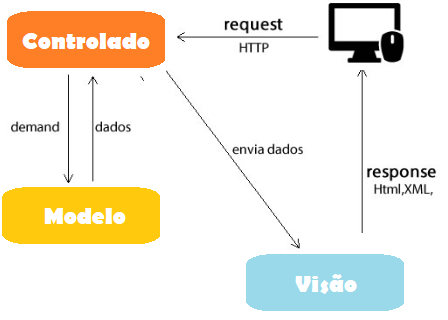
\includegraphics[width=9cm, height=5cm]{images/proposta-img/Figura4-1.png}
  \caption{Arquitetura}
  \label{fig:Figura4-1}
\end{center}
\end{figure}


\section{Casos de Uso}
\label{sc:casosDeUso}

Casos de Uso são técnicas introduzidas por  \citep{jacobson93} com o objetivo de descrever a interação entre o usuário e o sistema em cada funcionalidade. Nos casos mais simples, os casos de uso são compostos do seguintes elementos: os atores envolvidos em uma interação, a descrição da funcionalidade e a descrição da interação do ator com o sistema.

É possível representar um caso de uso utilizando um diagrama UML (linguagem de modelagem unificada, do inglês unified modeling language). A UML foi criada para estabelecer uma linguagem visual comum que pode ser compreendida por conhecedores da linguagem de programação e pessoas ligadas ao mundo dos negócios.

A figura \figref{fig:Figura4-2} apresenta o diagrama de casos de uso desta plataforma, nesse diagrama é possível verificar todas as funcionalidades do sistema e os usuários ligados a cada funcionalidade:

\begin{figure}[htp]
\begin{center}
  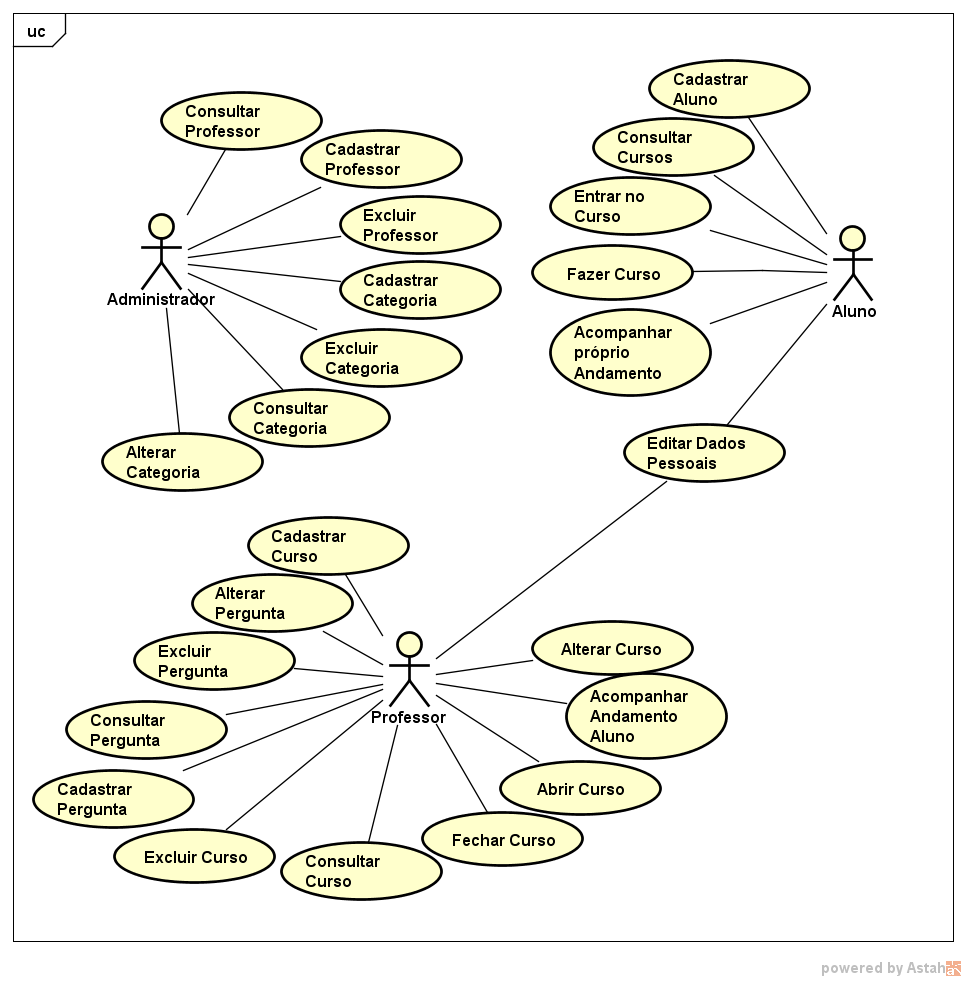
\includegraphics[width=15cm, height=18cm]{images/proposta-img/Figura4-2.png}
  \caption{Diagrama de Casos de Uso}
  \label{fig:Figura4-2}
\end{center}
\end{figure}

Os casos de uso foram descritos abaixo, utilizando os seguintes elementos:

\begin{itemize}
\item Ator Principal: representa o usuário que pode realizar a ação do caso de uso específico.
\item Resumo: contém um breve da ação realizada no caso.
\item Ações do Ator: Esse item representa a interação entre o autor e o sistema, para cada ação do autor deve ter alguma resposta do sistema.
\item Restrições e Validações: alguma restrição necessária para o usuário executar a ação.
\end{itemize}


\subsection{Caso de Uso 01 - Cadastrar Aluno}
\label{sc:case1}
\begin{center}
\begin{longtable}{p{8cm}|p{8cm}}
    \hline
    \textbf{Ator Principal} & Usu\'{a}rio \\
    \hline
    \textbf{Resumo} & O usuário fará seu cadastro no sistema \\
    \hline
    \textbf{Pr\'{e}-condi\c{c}\~{o}es} & 1. Usuário estar conectado à Internet\\
    \hline
    \textbf{A\c{c}\~{o}es do Ator} & \textbf{A\c{c}\~{o}es do Sistema} \\
    
    \hline
    1. Seleciona botão "Cadastrar" na tela de inicial & \\
    \hline
    2. Preencher os campos requisitados & \\
    \hline
    3. Seleciona botão "Cadastrar" para submeter os dados & \\
    \hline
    & 4. Envia os dados via web-service \\
    \hline
    & 5. Efetua o cadastro \\
    \hline
    \hline
    \textbf{Restri\c{c}\~{o}es/Valida\c{c}\~{o}es} & -------\\
\hline
\caption{Caso de Uso 01 - Cadastrar Usu\'{a}rio}
\end{longtable}
\end{center}

\subsection{Caso de Uso 02 - Cadastrar Professor}
\label{sc:case2}
\begin{center}
\begin{longtable}{p{8cm}|p{8cm}}
    \hline
    \textbf{Ator Principal} & Administrador \\
    \hline
    \textbf{Resumo} & O administrador fará o cadastro de um professor no sistema \\
    \hline
    \textbf{Pr\'{e}-condi\c{c}\~{o}es} & 1. Usuário estar logado no sistema; 2. Usuário ter o perfil de administrador \\
    \hline
    \textbf{A\c{c}\~{o}es do Ator} & \textbf{A\c{c}\~{o}es do Sistema} \\
    
    \hline
    1. Seleciona botão "Cadastrar Professor" na tela de inicial & \\
    \hline
    2. Preencher os campos requisitados & \\
    \hline
    3. Seleciona botão "Cadastrar" para submeter os dados & \\
    \hline
    & 4. Envia os dados via web-service \\
    \hline
    & 5. Efetua o cadastro \\
    \hline
    \hline
    \textbf{Restri\c{c}\~{o}es/Valida\c{c}\~{o}es} & -------\\
\hline
\caption{Caso de Uso 02 - Cadastrar Professor}
\end{longtable}
\end{center}

\subsection{Caso de Uso 03 - Fazer Login}
\label{sc:case3}
\begin{center}
\begin{longtable}{p{8cm}|p{8cm}}
    \hline
    \textbf{Ator Principal} & Usuário \\
    \hline
    \textbf{Resumo} & O usuário entrará no sistema \\
    \hline
    \textbf{Pr\'{e}-condi\c{c}\~{o}es} & 1. Usuário estar conectado à Internet \\
    \hline
    \textbf{A\c{c}\~{o}es do Ator} & \textbf{A\c{c}\~{o}es do Sistema} \\
    
    \hline
    1. Seleciona botão "Login" na tela de inicial & \\
    \hline
    2. Preencher o login e a senha & \\
    \hline
    3. Seleciona botão "Login" para submeter os dados & \\
    \hline
    & 4. Envia os dados via web-service \\
    \hline
    & 5. Validar se login e senha são válidos \\
    \hline
    & 6. Abrir sessão de acesso ao sistemas \\
    \hline
    \hline
    \textbf{Restri\c{c}\~{o}es/Valida\c{c}\~{o}es} & -------\\
\hline
\caption{Caso de Uso 03 - Fazer Login}
\end{longtable}
\end{center}


\subsection{Caso de Uso 04 - Fazer Logoff}
\label{sc:case4}
\begin{center}
\begin{longtable}{p{8cm}|p{8cm}}
    \hline
    \textbf{Ator Principal} & Usuário \\
    \hline
    \textbf{Resumo} & O usuário sairá do sistema \\
    \hline
    \textbf{Pr\'{e}-condi\c{c}\~{o}es} & 1. Usuário estar logado no sistema \\
    \hline
    \textbf{A\c{c}\~{o}es do Ator} & \textbf{A\c{c}\~{o}es do Sistema} \\
    
    \hline
    1. Seleciona botão "Sair" no menu & \\
    \hline
    & 2. Fechar a sessão do usuário \\
    \hline
    \hline
    \textbf{Restri\c{c}\~{o}es/Valida\c{c}\~{o}es} & -------\\
\hline
\caption{Caso de Uso 04 - Fazer Logoff}
\end{longtable}
\end{center}

\subsection{Caso de Uso 05 - Alterar Cadastro do Usuário}
\label{sc:case5}
\begin{center}
\begin{longtable}{p{8cm}|p{8cm}}
    \hline
    \textbf{Ator Principal} & Professor ou Aluno \\
    \hline
    \textbf{Resumo} & O usuário modificará algum dado do seu cadastro \\
    \hline
    \textbf{Pr\'{e}-condi\c{c}\~{o}es} & 1. Usuário estar logado no sistema \\
    \hline
    \textbf{A\c{c}\~{o}es do Ator} & \textbf{A\c{c}\~{o}es do Sistema} \\
    
    \hline
    1. Seleciona botão "Perfil" no menu & \\
    \hline
    2. Alterar algum dado do perfil2. Alterar algum dado do perfil \\
    \hline
    3. Seleciona botão "Salvar" para submeter os dados \\
    \hline
    & 4. Envia os dados via web-service \\
    \hline
    & 5. Efetuar edição do dados \\
    \hline
    & 6. Mensagem de dado editado com sucesso \\
    \hline
    \hline
    \textbf{Restri\c{c}\~{o}es/Valida\c{c}\~{o}es} & -------\\
\hline
\caption{Caso de Uso 05 - Alterar Cadastro do Usuário}
\end{longtable}
\end{center}


\subsection{Caso de Uso 06 - Cadastrar Pergunta}
\label{sc:case6}
\begin{center}
\begin{longtable}{p{8cm}|p{8cm}}
    \hline
    \textbf{Ator Principal} & Professor \\
    \hline
    \textbf{Resumo} & O professor fará o cadastro de uma pergunta no sistema \\
    \hline
    \textbf{Pr\'{e}-condi\c{c}\~{o}es} & 1. Usuário estar logado no sistema; 2. Usuário ter o perfil de professor \\
    \hline
    \textbf{A\c{c}\~{o}es do Ator} & \textbf{A\c{c}\~{o}es do Sistema} \\
    \hline
    1. Seleciona botão "Professor" no menu & \\
    \hline
    2. Seleciona a opção "Pergunta" \\
    \hline
    3. Seleciona botão "Nova Pergunta" \\
    \hline
    4. Preencher os campos obrigatórios \\
    \hline
    5. Seleciona botão "Salvar" \\
    \hline
    & 6. Envia os dados via web-service \\
	\hline
	& 7. Validar dados inseridos \\
	\hline
	& 8. Efetuar cadastro de pergunta \\
	\hline
	& 9. Exibir mensagem de pergunta salva com sucesso. \\
    \hline
    \hline
    \textbf{Restri\c{c}\~{o}es/Valida\c{c}\~{o}es} & -------\\
\hline
\caption{Caso de Uso 06 - Cadastrar Pergunta}
\end{longtable}
\end{center}

\subsection{Caso de Uso 07 - Alterar Pergunta}
\label{sc:case7}
\begin{center}
\begin{longtable}{p{8cm}|p{8cm}}
    \hline
    \textbf{Ator Principal} & Professor \\
    \hline
    \textbf{Resumo} & O professor vai alterar uma pergunta \\
    \hline
    \textbf{Pr\'{e}-condi\c{c}\~{o}es} & 1. Usuário estar logado no sistema; 2. Usuário ter o perfil de professor \\
    \hline
    \textbf{A\c{c}\~{o}es do Ator} & \textbf{A\c{c}\~{o}es do Sistema} \\
    \hline
    1. Seleciona botão "Professor" no menu \\
    \hline
    2. Seleciona a opção "Pergunta" \\
	\hline
    3. Pesquisar uma pergunta \\
	\hline
    4. Selecionar o lápis (Editar) \\
	\hline
    5. Editar os dados \\
	\hline
    6. Seleciona botão "Salvar" \\
    \hline
    & 7. Envia os dados via web-service \\
	\hline
    & 8. Efetuar edição da pergunta \\
	\hline
    & 9. Exibir mensagem de pergunta salva com sucesso. \\
    \hline
    \hline
    \textbf{Restri\c{c}\~{o}es/Valida\c{c}\~{o}es} & 1. A pergunta deverá ter sido criada pelo professor; 2. A pergunta não pode está associada a nenhum curso \\
\hline
\caption{Caso de Uso 07 - Alterar Pergunta}
\end{longtable}
\end{center}

\subsection{Caso de Uso 08 - Excluir Pergunta}
\label{sc:case8}
\begin{center}
\begin{longtable}{p{8cm}|p{8cm}}
    \hline
    \textbf{Ator Principal} & Professor \\
    \hline
    \textbf{Resumo} & O professor vai excluir uma pergunta \\
    \hline
    \textbf{Pr\'{e}-condi\c{c}\~{o}es} & 1. Usuário estar logado no sistema; 2. Usuário ter o perfil de professor \\
    \hline
    \textbf{A\c{c}\~{o}es do Ator} & \textbf{A\c{c}\~{o}es do Sistema} \\
    \hline
    1. Seleciona botão "Professor" no menu \\
    \hline
    2. Seleciona a opção "Pergunta" \\
	\hline
    3. Pesquisar uma pergunta \\
	\hline
    4. Selecionar o ‘x’ (Excluir) \\
    \hline
    & 5. Envia os dados via web-service \\
	\hline
    & 6 Efetuar exclusão da pergunta \\
	\hline
    & 7. Exibir mensagem de pergunta excluída com sucesso. \\
    \hline
    \hline
    \textbf{Restri\c{c}\~{o}es/Valida\c{c}\~{o}es} & 1. A pergunta deverá ter sido criada pelo professor; 2. A pergunta não pode está associada a nenhum curso \\
\hline
\caption{Caso de Uso 08 - Excluir Pergunta}
\end{longtable}
\end{center}


\subsection{Caso de Uso 09 - Consultar Pergunta}
\label{sc:case9}
\begin{center}
\begin{longtable}{p{8cm}|p{8cm}}
    \hline
    \textbf{Ator Principal} & Professor \\
    \hline
    \textbf{Resumo} & O professor vai consultar uma pergunta \\
    \hline
    \textbf{Pr\'{e}-condi\c{c}\~{o}es} & 1. Usuário estar logado no sistema; 2. Usuário ter o perfil de professor \\
    \hline
    \textbf{A\c{c}\~{o}es do Ator} & \textbf{A\c{c}\~{o}es do Sistema} \\
    \hline
    1. Seleciona botão "Professor" no menu \\
    \hline
    2. Seleciona a opção "Pergunta" \\
	\hline
    3. Selecionar o filtro desejado \\
	\hline
    4. Seleciona botão "Pesquisar" \\
    \hline
    & 5. Envia os dados via web-service \\
	\hline
    & 6. Efetuar a pesquisa \\
	\hline
    & 7. Retornar dados para tela \\
	\hline
    & 9. Exibir dados na grid \\
    \hline
    \hline
    \textbf{Restri\c{c}\~{o}es/Valida\c{c}\~{o}es} & -------\\
\hline
\caption{Caso de Uso 09 - Consultar Pergunta}
\end{longtable}
\end{center}

\subsection{Caso de Uso 10 - Cadastrar Curso}
\label{sc:case10}
\begin{center}
\begin{longtable}{p{8cm}|p{8cm}}
    \hline
    \textbf{Ator Principal} & Professor \\
    \hline
    \textbf{Resumo} & O professor fará o cadastro de um curso com etapas no sistema \\
    \hline
    \textbf{Pr\'{e}-condi\c{c}\~{o}es} & 1. Usuário estar logado no sistema; 2. Usuário ter o perfil de professor \\
    \hline
    \textbf{A\c{c}\~{o}es do Ator} & \textbf{A\c{c}\~{o}es do Sistema} \\
    \hline
    1. Seleciona botão "Professor" no menu \\
    \hline
    2. Seleciona a opção "Criar Curso" \\
	\hline
    4. Preencher os campos obrigatórios \\
	\hline
    5. Seleciona botão "Próximo" \\
    \hline
    & 6. Envia os dados via web-service \\
	\hline
    & 7. Efetuar cadastro do curso no banco de dados \\
	\hline
    & 8. Enviar o professor para tela de adicionar etapas \\
	\hline
    9. Preencher os campos obrigatórios da etapa \\
	\hline
    10. Seleciona a opção "Adicionar Perguntas" \\
	\hline
    11. Pesquisar perguntas \\
	\hline
    12. Selecionar perguntas escolhidas \\
	\hline
    13. Seleciona botão "Adicionar" \\
	\hline
    14. Selecionar o botão “Próximo Etapa” ou “Concluir” \\
	\hline
    & 15. Envia os dados via web-service \\
    \hline
    \hline
    \textbf{Restri\c{c}\~{o}es/Valida\c{c}\~{o}es} & -------\\
\hline
\caption{Caso de Uso 10 - Cadastrar Curso}
\end{longtable}
\end{center}

\subsection{Caso de Uso 11 - Alterar Curso}
\label{sc:case11}
\begin{center}
\begin{longtable}{p{8cm}|p{8cm}}
    \hline
    \textbf{Ator Principal} & Professor \\
    \hline
    \textbf{Resumo} & O professor vai alterar um curso \\
    \hline
    \textbf{Pr\'{e}-condi\c{c}\~{o}es} & 1. Usuário estar logado no sistema; 2. Usuário ter o perfil de professor \\
    \hline
    \textbf{A\c{c}\~{o}es do Ator} & \textbf{A\c{c}\~{o}es do Sistema} \\
    \hline
    1. Seleciona botão "Professor" no menu \\
    \hline
    2. Seleciona a opção "Cursos que Criei" \\
	\hline
    3. Pesquisar um curso \\
	\hline
    4. Selecionar o lápis (Editar) \\
	\hline
    5. Editar os dados \\
	\hline
    6. Selecionar o botão “Próximo” ou “Concluir” \\
    \hline
    & 7. Envia os dados via web-service \\
	\hline
    & 8. Efetuar edição do curso \\
	\hline
    & 9. Exibir mensagem de curso salvo com sucesso \\
    \hline
    \hline
    \textbf{Restri\c{c}\~{o}es/Valida\c{c}\~{o}es} & 1. O curso deverá ter sido criada pelo professor; 2. O curso não pode está com situação concluído \\
\hline
\caption{Caso de Uso 11 - Alterar Curso}
\end{longtable}
\end{center}

\subsection{Caso de Uso 12 - Excluir Curso}
\label{sc:case12}
\begin{center}
\begin{longtable}{p{8cm}|p{8cm}}
    \hline
    \textbf{Ator Principal} & Professor \\
    \hline
    \textbf{Resumo} & O professor vai excluir um curso \\
    \hline
    \textbf{Pr\'{e}-condi\c{c}\~{o}es} & 1. Usuário estar logado no sistema; 2. Usuário ter o perfil de professor \\
    \hline
    \textbf{A\c{c}\~{o}es do Ator} & \textbf{A\c{c}\~{o}es do Sistema} \\
    \hline
    1. Seleciona botão "Professor" no menu \\
    \hline
    2. Seleciona a opção "Cursos que Criei" \\
	\hline
    3. Pesquisar um curso \\
	\hline
    4. Selecionar o ‘x’ (Excluir) \\
    \hline
    & 5. Envia os dados via web-service \\
	\hline
    & 6. Efetuar exclusão do curso do banco de dados \\
	\hline
    & 7. Exibir mensagem de curso excluído com sucesso. \\
    \hline
    \hline
    \textbf{Restri\c{c}\~{o}es/Valida\c{c}\~{o}es} & 1. O curso deverá ter sido criada pelo professor logado; 2. O curso não pode está associada a nenhum aluno \\
\hline
\caption{Caso de Uso 12 - Excluir Curso}
\end{longtable}
\end{center}

\subsection{Caso de Uso 13 - Consultar Curso}
\label{sc:case13}
\begin{center}
\begin{longtable}{p{8cm}|p{8cm}}
    \hline
    \textbf{Ator Principal} & Professor \\
    \hline
    \textbf{Resumo} & O professor vai consultar um curso \\
    \hline
    \textbf{Pr\'{e}-condi\c{c}\~{o}es} & 1. Usuário estar logado no sistema; 2. Usuário ter o perfil de professor \\
    \hline
    \textbf{A\c{c}\~{o}es do Ator} & \textbf{A\c{c}\~{o}es do Sistema} \\
    \hline
    1. Seleciona botão "Professor" no menu \\
    \hline
    2. Seleciona a opção "Cursos que Criei" \\
	\hline
    3. Selecionar o filtro desejado \\
	\hline
    4. Seleciona botão "Pesquisar" \\
    \hline
    & 5. Envia os dados via web-service \\
	\hline
    & 6. Efetuar a pesquisa \\
	\hline
    & 7. Retornar dados para tela \\
	\hline
    & 9. Exibir dados na grid \\
    \hline
    \hline
    \textbf{Restri\c{c}\~{o}es/Valida\c{c}\~{o}es} & -------\\
\hline
\caption{Caso de Uso 13 - Consultar Curso}
\end{longtable}
\end{center}

\subsection{Caso de Uso 14 - Acompanhar andamento dos alunos}
\label{sc:case10}
\begin{center}
\begin{longtable}{p{8cm}|p{8cm}}
    \hline
    \textbf{Ator Principal} & Professor \\
    \hline
    \textbf{Resumo} & O professor vai acompanhar o andamento dos alunos \\
    \hline
    \textbf{Pr\'{e}-condi\c{c}\~{o}es} & 1. Usuário estar logado no sistema; 2. Usuário ter o perfil de professor \\
    \hline
    \textbf{A\c{c}\~{o}es do Ator} & \textbf{A\c{c}\~{o}es do Sistema} \\
    \hline
    1. Seleciona botão "Professor" no menu \\
    \hline
    2. Seleciona a opção "Cursos que Criei" \\
	\hline
    3. Selecionar o filtro desejado \\
	\hline
    4. Seleciona botão "Pesquisar" \\
	\hline
    5. Selecionar a lupa do curso que deseja ver o andamento dos alunos \\
    \hline
    & 5. Envia os dados do curso via web-service \\
	\hline
    & 6. Efetuar a pesquisa do andamento do aluno \\
	\hline
    & 7. Retornar dados para o front-end \\
	\hline
    & 8. Exibir dados na tela \\
    \hline
    \hline
    \textbf{Restri\c{c}\~{o}es/Valida\c{c}\~{o}es} & -------\\
\hline
\caption{Caso de Uso 14 - Acompanhar andamento dos alunos}
\end{longtable}
\end{center}

\subsection{Caso de Uso 15 - Entrar em Curso}
\label{sc:case15}
\begin{center}
\begin{longtable}{p{8cm}|p{8cm}}
    \hline
    \textbf{Ator Principal} & Aluno \\
    \hline
    \textbf{Resumo} & O aluno entrará no curso \\
    \hline
    \textbf{Pr\'{e}-condi\c{c}\~{o}es} & 1. Usuário estar logado no sistema; 2. Usuário ter o perfil de aluno \\
    \hline
    \textbf{A\c{c}\~{o}es do Ator} & \textbf{A\c{c}\~{o}es do Sistema} \\
    \hline
    1. Seleciona botão "Aluno" no menu \\
    \hline
    2. Seleciona a opção "Consultar Cursos" \\
	\hline
    3. Selecionar o filtro desejado \\
	\hline
    4. Seleciona botão "Pesquisar" \\
	\hline
    5. Selecionar a opção “Entrar” na grid \\
    \hline
    & 6. Envia os dados do curso via web-service \\
	\hline
    & 7. Efetuar a pesquisa dos dados do curso \\
	\hline
    & 8. Retornar dados para o front-end \\
	\hline
    & 9. Exibir dados na tela \\
	\hline
    10. Inserir o Código de Acesso \\
	\hline
    11. Seleciona botão "Entrar" \\
	\hline
    & 12. Envia os dados via web-service \\
	\hline
    & 13. Validar código de acesso \\
	\hline
    & 14. Associar aluno ao curso \\
	\hline
    & 15. Direcionar o aluno a tela do curso \\
    \hline
    \hline
    \textbf{Restri\c{c}\~{o}es/Valida\c{c}\~{o}es} & -------\\
\hline
\caption{Caso de Uso 15 - Entrar em Curso}
\end{longtable}
\end{center}

\subsection{Caso de Uso 16 - Fazer Curso}
\label{sc:case16}
\begin{center}
\begin{longtable}{p{8cm}|p{8cm}}
    \hline
    \textbf{Ator Principal} & Aluno \\
    \hline
    \textbf{Resumo} & O aluno passará pelas etapas do curso \\
    \hline
    \textbf{Pr\'{e}-condi\c{c}\~{o}es} & 1. Usuário estar logado no sistema; 2. Usuário ter o perfil de aluno; 3. O aluno está associado ao curso \\
    \hline
    \textbf{A\c{c}\~{o}es do Ator} & \textbf{A\c{c}\~{o}es do Sistema} \\
    \hline
    1. Seleciona botão "Aluno" no menu \\
    \hline
    2. Seleciona a opção "Meus Cursos" \\
	\hline
    3. Selecionar “Cursos em Andamento” \\
	\hline
    4. Selecionar o curso que deseja  \\
	\hline
    5. Selecionar a opção “Entrar” na grid \\
    \hline
    & 6. Envia os dados do curso via web-service \\
	\hline
    & 7. Efetuar a pesquisa dos dados do curso \\
	\hline
    & 8. Retornar dados para o front-end \\
	\hline
    & 9. Exibir dados na tela \\
	\hline
    10. Inserir o Código de Acesso \\
	\hline
    11. Seleciona botão "Entrar" \\
	\hline
    12. Envia os dados via web-service \\
    \hline
    13. Validar código de acesso \\
	\hline
    14. Associar aluno ao curso \\
	\hline
    15. Direcionar o aluno a tela do curso \\
    \hline
    \hline
    \textbf{Restri\c{c}\~{o}es/Valida\c{c}\~{o}es} & -------\\
\hline
\caption{Caso de Uso 16 - Fazer Curso}
\end{longtable}
\end{center}

\subsection{Caso de Uso 17 - Acompanhar próprio andamento}
\label{sc:case17}
\begin{center}
\begin{longtable}{p{8cm}|p{8cm}}
    \hline
    \textbf{Ator Principal} & Aluno \\
    \hline
    \textbf{Resumo} & O aluno acompanhará o seu próprio andamento em cada curso que ele participa \\
    \hline
    \textbf{Pr\'{e}-condi\c{c}\~{o}es} & 1. Usuário estar logado no sistema; 2. Usuário ter o perfil de aluno \\
    \hline
    \textbf{A\c{c}\~{o}es do Ator} & \textbf{A\c{c}\~{o}es do Sistema} \\
    \hline
    1. Seleciona botão "Aluno" no menu \\
    \hline
    2. Seleciona a opção "Meus Cursos" \\
	\hline
    3. Selecionar “Cursos em Andamento” \\
	\hline
    4. Selecionar o curso que deseja  \\
    \hline
    & 5. Direciona o aluno para a página do curso \\
	\hline
    6. Seleciona o “Andamento” \\
	\hline
    & 7. Exibir andamento na tela \\
    \hline
    \hline
    \textbf{Restri\c{c}\~{o}es/Valida\c{c}\~{o}es} & -------\\
\hline
\caption{Caso de Uso 17 - Acompanhar próprio andamento}
\end{longtable}
\end{center}

\subsection{Caso de Uso 18 - Cadastrar Categorias de Perguntas}
\label{sc:case18}
\begin{center}
\begin{longtable}{p{8cm}|p{8cm}}
    \hline
    \textbf{Ator Principal} & Administrador \\
    \hline
    \textbf{Resumo} & O administrador fará o cadastro de uma categoria da pergunta no sistema \\
    \hline
    \textbf{Pr\'{e}-condi\c{c}\~{o}es} & 1. Usuário estar logado no sistema; 2. Usuário ter o perfil de administrador \\
    \hline
    \textbf{A\c{c}\~{o}es do Ator} & \textbf{A\c{c}\~{o}es do Sistema} \\
    \hline
    1. Seleciona botão "Administrador" no menu \\
    \hline
    2. Seleciona a opção "Categoria" \\
	\hline
    3. Seleciona botão "Nova Categoria" \\
	\hline
    4. Preencher os campos obrigatórios \\
	\hline
    5. Seleciona botão "Salvar" \\
    \hline
    & 6. Envia os dados via web-service \\
	\hline
    & 7. Validar dados inseridos \\
	\hline
    & 8. Efetuar cadastro da categoria da pergunta \\
	\hline
    & 9. Exibir mensagem de categoria da pergunta salva com sucesso. \\
    \hline
    \hline
    \textbf{Restri\c{c}\~{o}es/Valida\c{c}\~{o}es} & -------\\
\hline
\caption{Caso de Uso 18 - Cadastrar Categorias de Perguntas}
\end{longtable}
\end{center}

\subsection{Caso de Uso 19 - Alterar Categorias de Perguntas}
\label{sc:case19}
\begin{center}
\begin{longtable}{p{8cm}|p{8cm}}
    \hline
    \textbf{Ator Principal} & Administrador \\
    \hline
    \textbf{Resumo} & O administrador vai alterar uma categoria \\
    \hline
    \textbf{Pr\'{e}-condi\c{c}\~{o}es} & 1. Usuário estar logado no sistema; 2. Usuário ter o perfil de administrador \\
    \hline
    \textbf{A\c{c}\~{o}es do Ator} & \textbf{A\c{c}\~{o}es do Sistema} \\
    \hline
    1. Seleciona botão "Administrador" no menu \\
    \hline
    2. Seleciona a opção "Categoria" \\
	\hline
    3. Pesquisar uma categoria \\
	\hline
    4. Selecionar o lápis (Editar) \\
	\hline
    5. Editar os dados \\
	\hline
    6. Seleciona botão "Salvar" \\
    \hline
    & 7. Envia os dados via web-service \\
	\hline
    & 8. Efetuar edição da categoria \\
	\hline
    & 9. Exibir mensagem de categoria salva com sucesso. \\
    \hline
    \hline
    \textbf{Restri\c{c}\~{o}es/Valida\c{c}\~{o}es} & -------\\
\hline
\caption{Caso de Uso 19 - Alterar Categorias de Perguntas}
\end{longtable}
\end{center}

\subsection{Caso de Uso 20 - Excluir Categorias de Perguntas}
\label{sc:case20}
\begin{center}
\begin{longtable}{p{8cm}|p{8cm}}
    \hline
    \textbf{Ator Principal} & Administrador \\
    \hline
    \textbf{Resumo} & O administrador vai excluir uma categoria \\
    \hline
    \textbf{Pr\'{e}-condi\c{c}\~{o}es} & 1. Usuário estar logado no sistema; 2. Usuário ter o perfil de administrador \\
    \hline
    \textbf{A\c{c}\~{o}es do Ator} & \textbf{A\c{c}\~{o}es do Sistema} \\
    \hline
    1. Seleciona botão "Administrador" no menu \\
    \hline
    2. Seleciona a opção "Categoria" \\
	\hline
    3. Pesquisar uma categoria \\
	\hline
    4. Selecionar o ‘x’ (Excluir) \\
    \hline
    & 5. Envia os dados via web-service \\
	\hline
    & 6. Efetuar exclusão da categoria \\
	\hline
    & 7. Exibir mensagem de categoria excluída com sucesso. \\
    \hline
    \hline
    \textbf{Restri\c{c}\~{o}es/Valida\c{c}\~{o}es} & 1. A categoria não pode está associada a nenhuma pergunta\\
\hline
\caption{Caso de Uso 20 - Excluir Categorias de Perguntas}
\end{longtable}
\end{center}

\subsection{Caso de Uso 21 - Consultar Categorias de Perguntas}
\label{sc:case21}
\begin{center}
\begin{longtable}{p{8cm}|p{8cm}}
    \hline
    \textbf{Ator Principal} & Professor \\
    \hline
    \textbf{Resumo} & O professor vai consultar uma pergunta \\
    \hline
    \textbf{Pr\'{e}-condi\c{c}\~{o}es} & 1. Usuário estar logado no sistema; 2. Usuário ter o perfil de professor \\
    \hline
    \textbf{A\c{c}\~{o}es do Ator} & \textbf{A\c{c}\~{o}es do Sistema} \\
    \hline
    1. Seleciona botão "Professor" no menu \\
    \hline
    2. Seleciona a opção "Pergunta" \\
	\hline
    3. Selecionar o filtro desejado \\
	\hline
    4. Seleciona botão "Pesquisar" \\
    \hline
    & 5. Envia os dados via web-service \\
	\hline
    & 6. Efetuar a pesquisa \\
	\hline
    & 7. Retornar dados para tela \\
	\hline
    & 8. Exibir dados na grid \\
    \hline
    \hline
    \textbf{Restri\c{c}\~{o}es/Valida\c{c}\~{o}es} & -------\\
\hline
\caption{Caso de Uso 21 - Consultar Categorias de Perguntas}
\end{longtable}
\end{center}



\section{Diagrama de Sequência}
\label{sc:diagramaSequencia}

A sequência de interações entre os usuários e o sistema definidos em um caso de uso pode ser mostrado por meio de um diagrama de sequência. É interessante fazer uso deste recurso quando as funcionalidades são complexas pois ele tem a finalidade auxilia no entendimento geral. \citep{SOMMERVILLE2011}.

As subseções que se seguem mostram os diagramas de sequência dos principais casos de uso da plataforma.

\subsection{Diagrama de Sequência 01 - Cadastro de Professor}
A figura \figref{fig:Figura4-3} apresenta o diagrama de sequência do caso de uso mostrado na seção \ref{sc:case2}.
\begin{figure}[h]
\begin{center}
  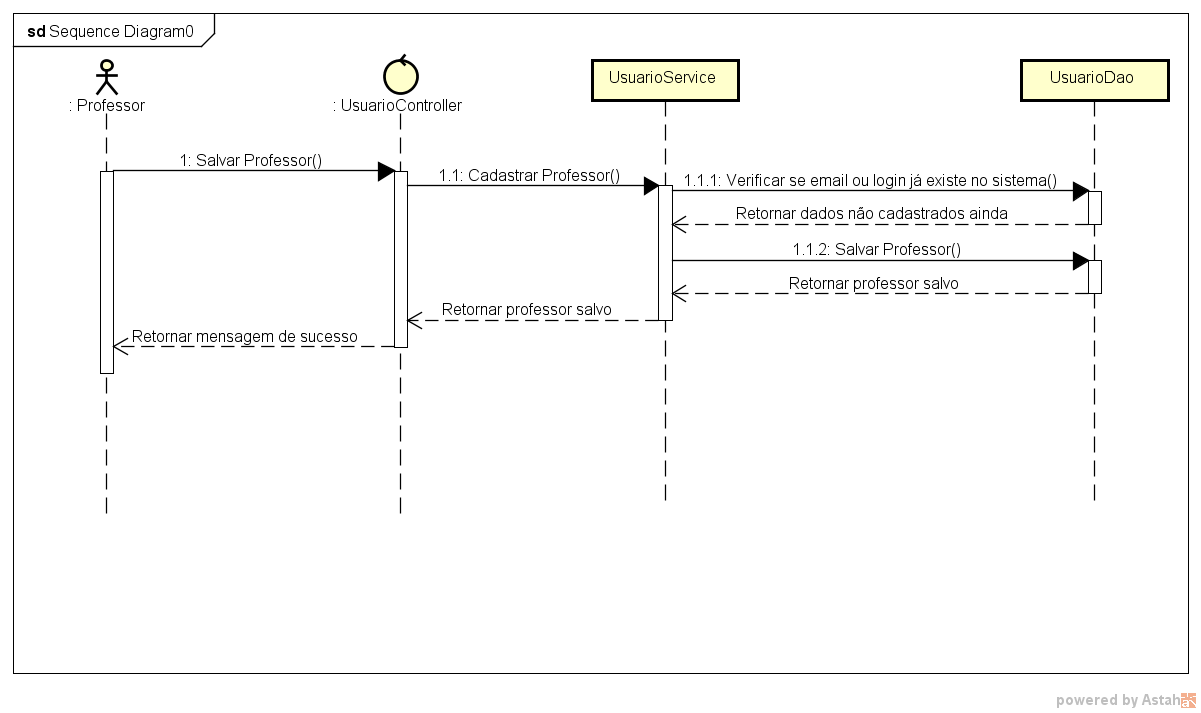
\includegraphics[width=15cm, height=6cm]{images/proposta-img/Figura4-3.png}
  \caption{Cadastro de Professor}
  \label{fig:Figura4-3}
\end{center}
\end{figure}
\subsection{Diagrama de Sequência 02 - Cadastro de Aluno}
A figura \figref{fig:Figura4-4} apresenta o diagrama de sequência do caso de uso mostrado na seção \ref{sc:case1}.
\begin{figure}[htp]
\begin{center}
  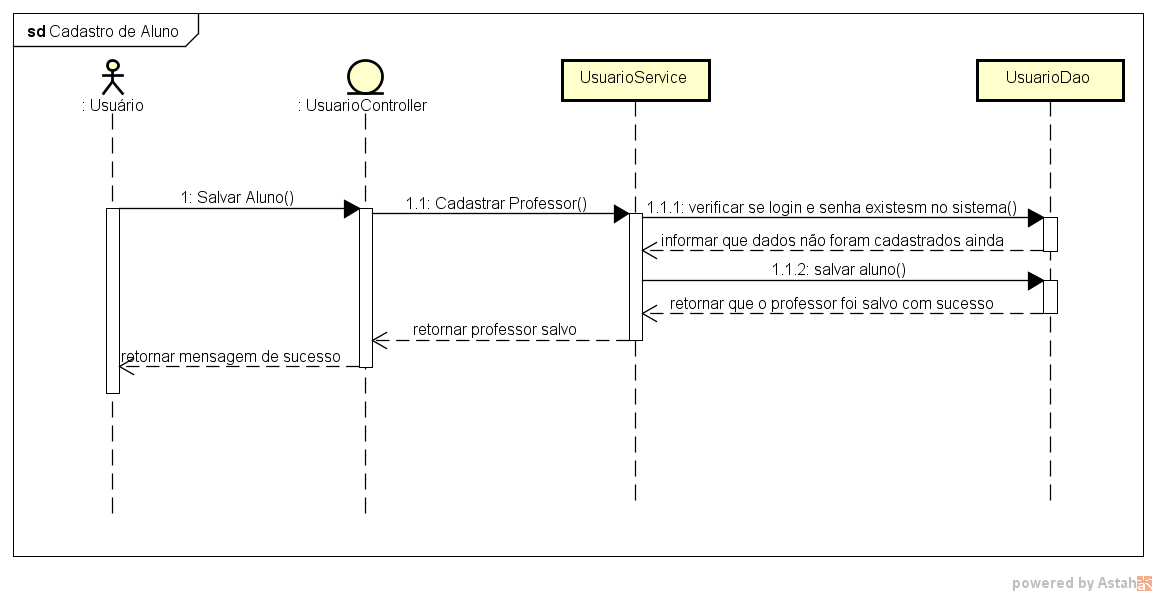
\includegraphics[width=15cm, height=6cm]{images/proposta-img/Figura4-4.png}
  \caption{Cadastro de Aluno}
  \label{fig:Figura4-4}
\end{center}
\end{figure}
\subsection{Diagrama de Sequência 03 - Cadastro de Pergunta}
A figura \figref{fig:Figura4-5} apresenta o diagrama de sequência do caso de uso mostrado na seção \ref{sc:case6}.
\begin{figure}[htp]
\begin{center}
  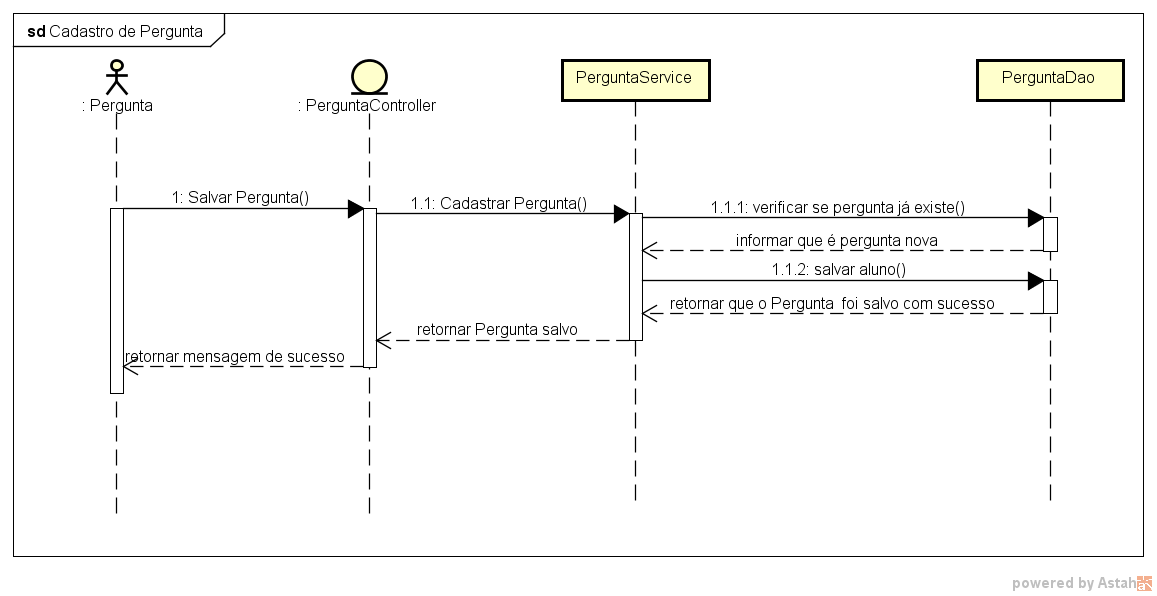
\includegraphics[width=15cm, height=6cm]{images/proposta-img/Figura4-5.png}
  \caption{Cadastro de Pergunta}
  \label{fig:Figura4-5}
\end{center}
\end{figure}
\subsection{Diagrama de Sequência 04 - Cadastro de Curso}
A figura \figref{fig:Figura4-6} apresenta o diagrama de sequência do caso de uso mostrado na seção \ref{sc:case10}.
\begin{figure}[htp]
\begin{center}
  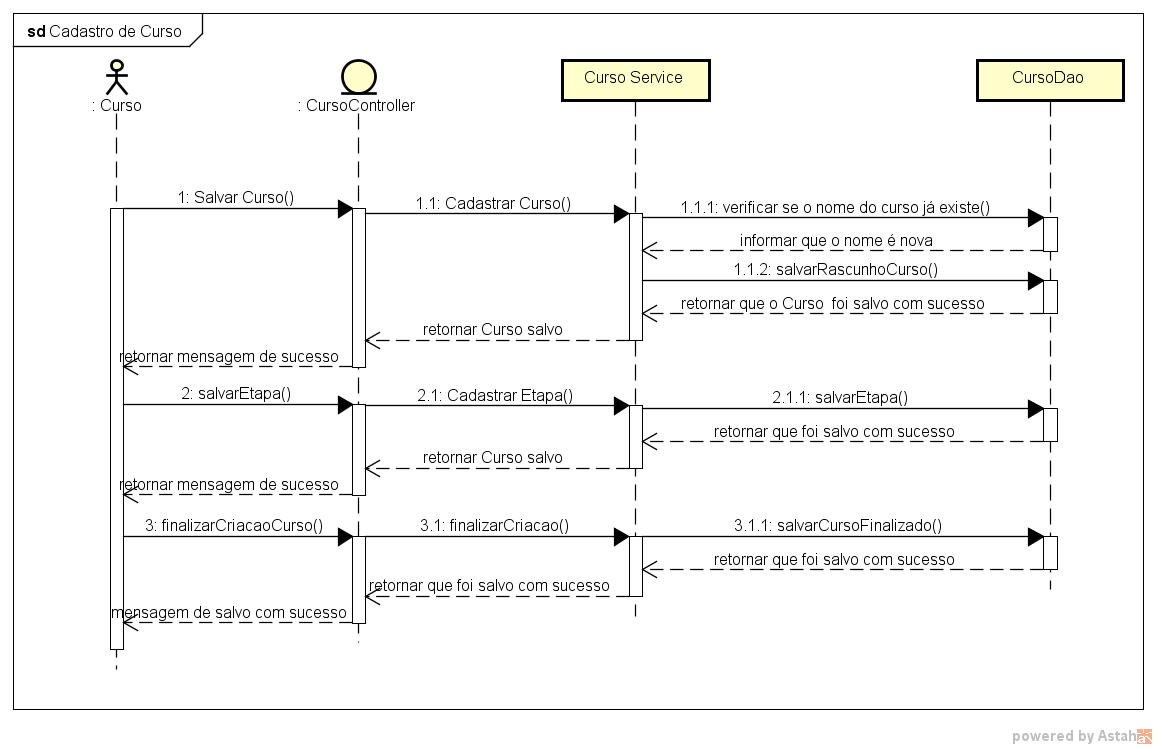
\includegraphics[width=15cm, height=6cm]{images/proposta-img/Figura4-6.png}
  \caption{Cadastro de Curso}
  \label{fig:Figura4-6}
\end{center}
\end{figure}


\section{Diagrama de classes}

Todos cenários de caso de uso implicam em um conjunto de objetos manipulados à medida que um ator interage com o sistema. Esses objetos são categorizados em classes — um conjunto de coisas que possuem atributos similares e comportamentos comuns. \citep{SOMMERVILLE2011}

Na \figref{fig:Figura4-7} é possível identificar  todas as classes da plataforma através do diagrama UML de classe da apresentado.

\begin{figure}[htp]
\begin{center}
  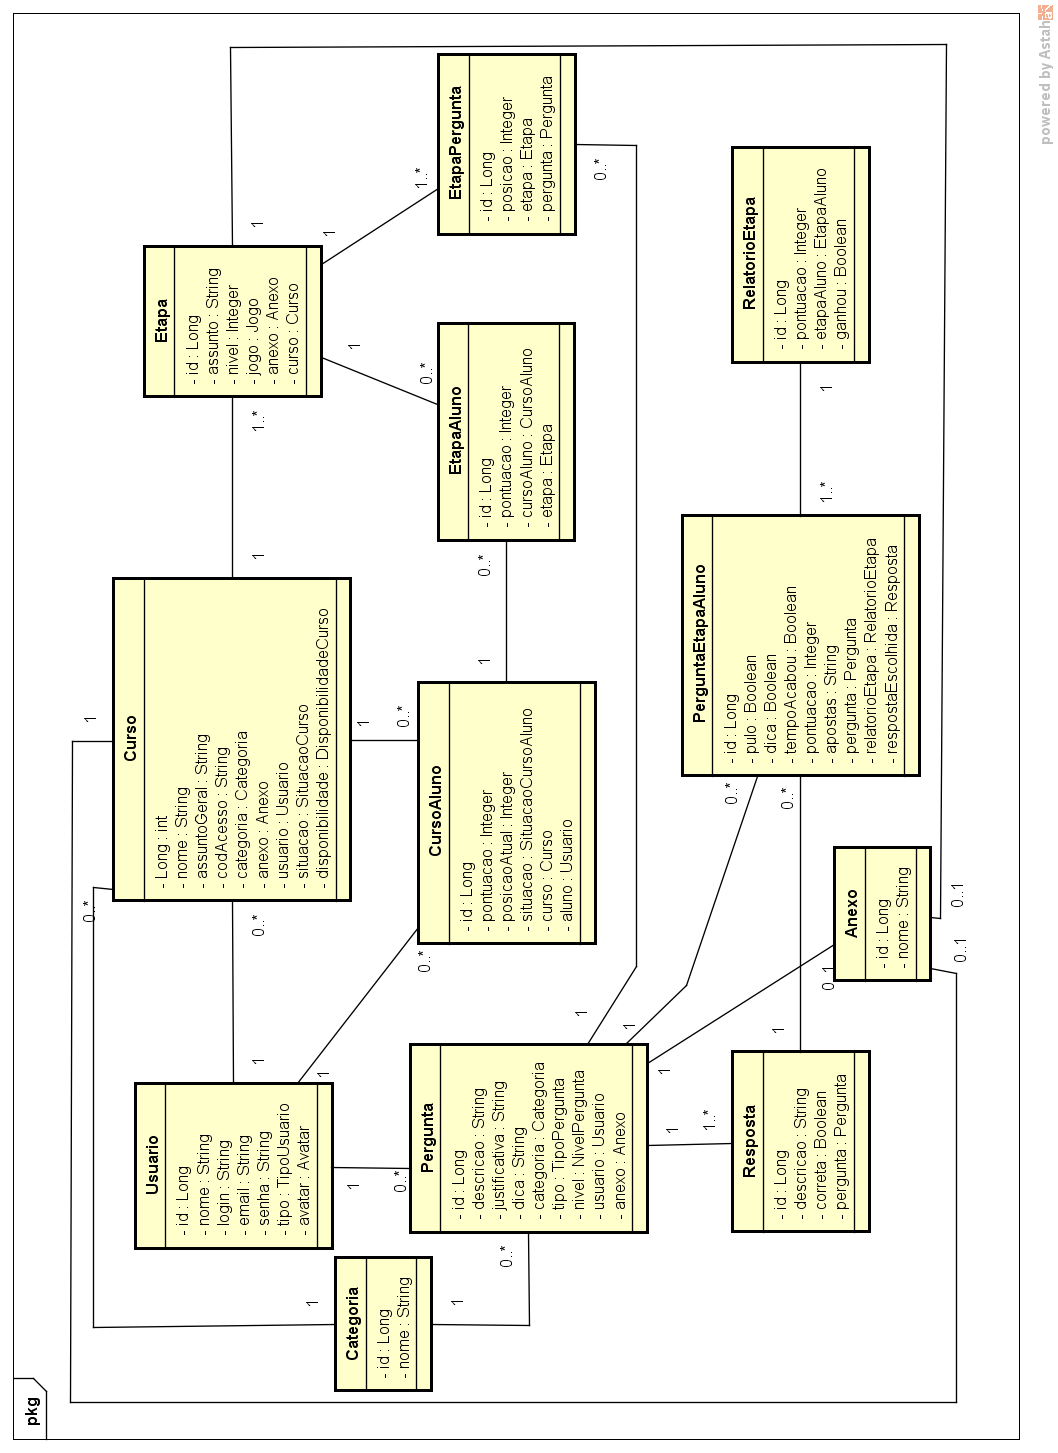
\includegraphics[width=15cm, height=15cm]{images/proposta-img/Figura4-7.png}
  \caption{Diagrama de classes}
  \label{fig:Figura4-7}
\end{center}
\end{figure}


\section{Telas e Funcionalidades}

\subsection{Descrição Geral}

A plataforma GameInfor  tem três tipos de usuários: 1) administrador - ele pode criar professores e categorias, 2) o professor - ele tem a capacidade de criar perguntas, cursos e acompanhar o andamento dos alunos; 3) o aluno - este grupo participa dos cursos oferecidos no site.  

Aprofundando a análise das funcionalidades, destaca-se que o professor criará uma sequência de aulas organizadas por níveis de conhecimento, sendo que ao aluno somente será permitido passar para um nível mais elevado após atingir determinada quantidade de pontos na atual fase. Além disso, cada etapa será composta de um texto e/ou imagem do conteúdo da aula, e ainda incluirá um jogo vinculado a este assunto abordado.

Inicialmente estarão disponíveis os seguintes jogos para o usuário: aposta, quiz, caça palavras, jogo da forca e jogo da velha. Com o propósito de aumentar a curva de aprendizagem do conteúdo, o aluno que participar dos jogos da plataforma, receberá, no final do desafio, um relatório com todas as explicações das perguntas constantes na partida. E, ainda, haverá um ranking mostrando os melhores jogadores.

A plataforma disponibilizará na sua versão beta os jogos supracitados, todavia, caso o desenvolvedor deseje acrescentar novas atividades utilizando os conceitos de gamificação, a plataforma dará o suporte necessário. O projeto, nesse sentido, será construído de modo flexível e intuitiva.

A plataforma também disponibiliza manuais para todos os três tipos de usuários existentes e antes de cada jogo, o aluno pode visualizar uma breve explicação do funcionamento do mesmo.


\subsection{Acessar a plataforma}

É possível acessar a plataforma GameInfor através do link gameinfor.net. Nesta tela o usuário encontrará a opção de logar no sistema e de se cadastrar. É importante ressaltar que todo usuário cadastrado no sistema através do botão "Cadastrar" encontrado nesta tela, recebe o perfil de aluno. O cadastro de professor será mostrado na seção XX. O sistema não disponibiliza cadastros de administradores, usuário com esse perfil só pode ser inserido via banco de dados.

\begin{figure}[h]
\begin{center}
  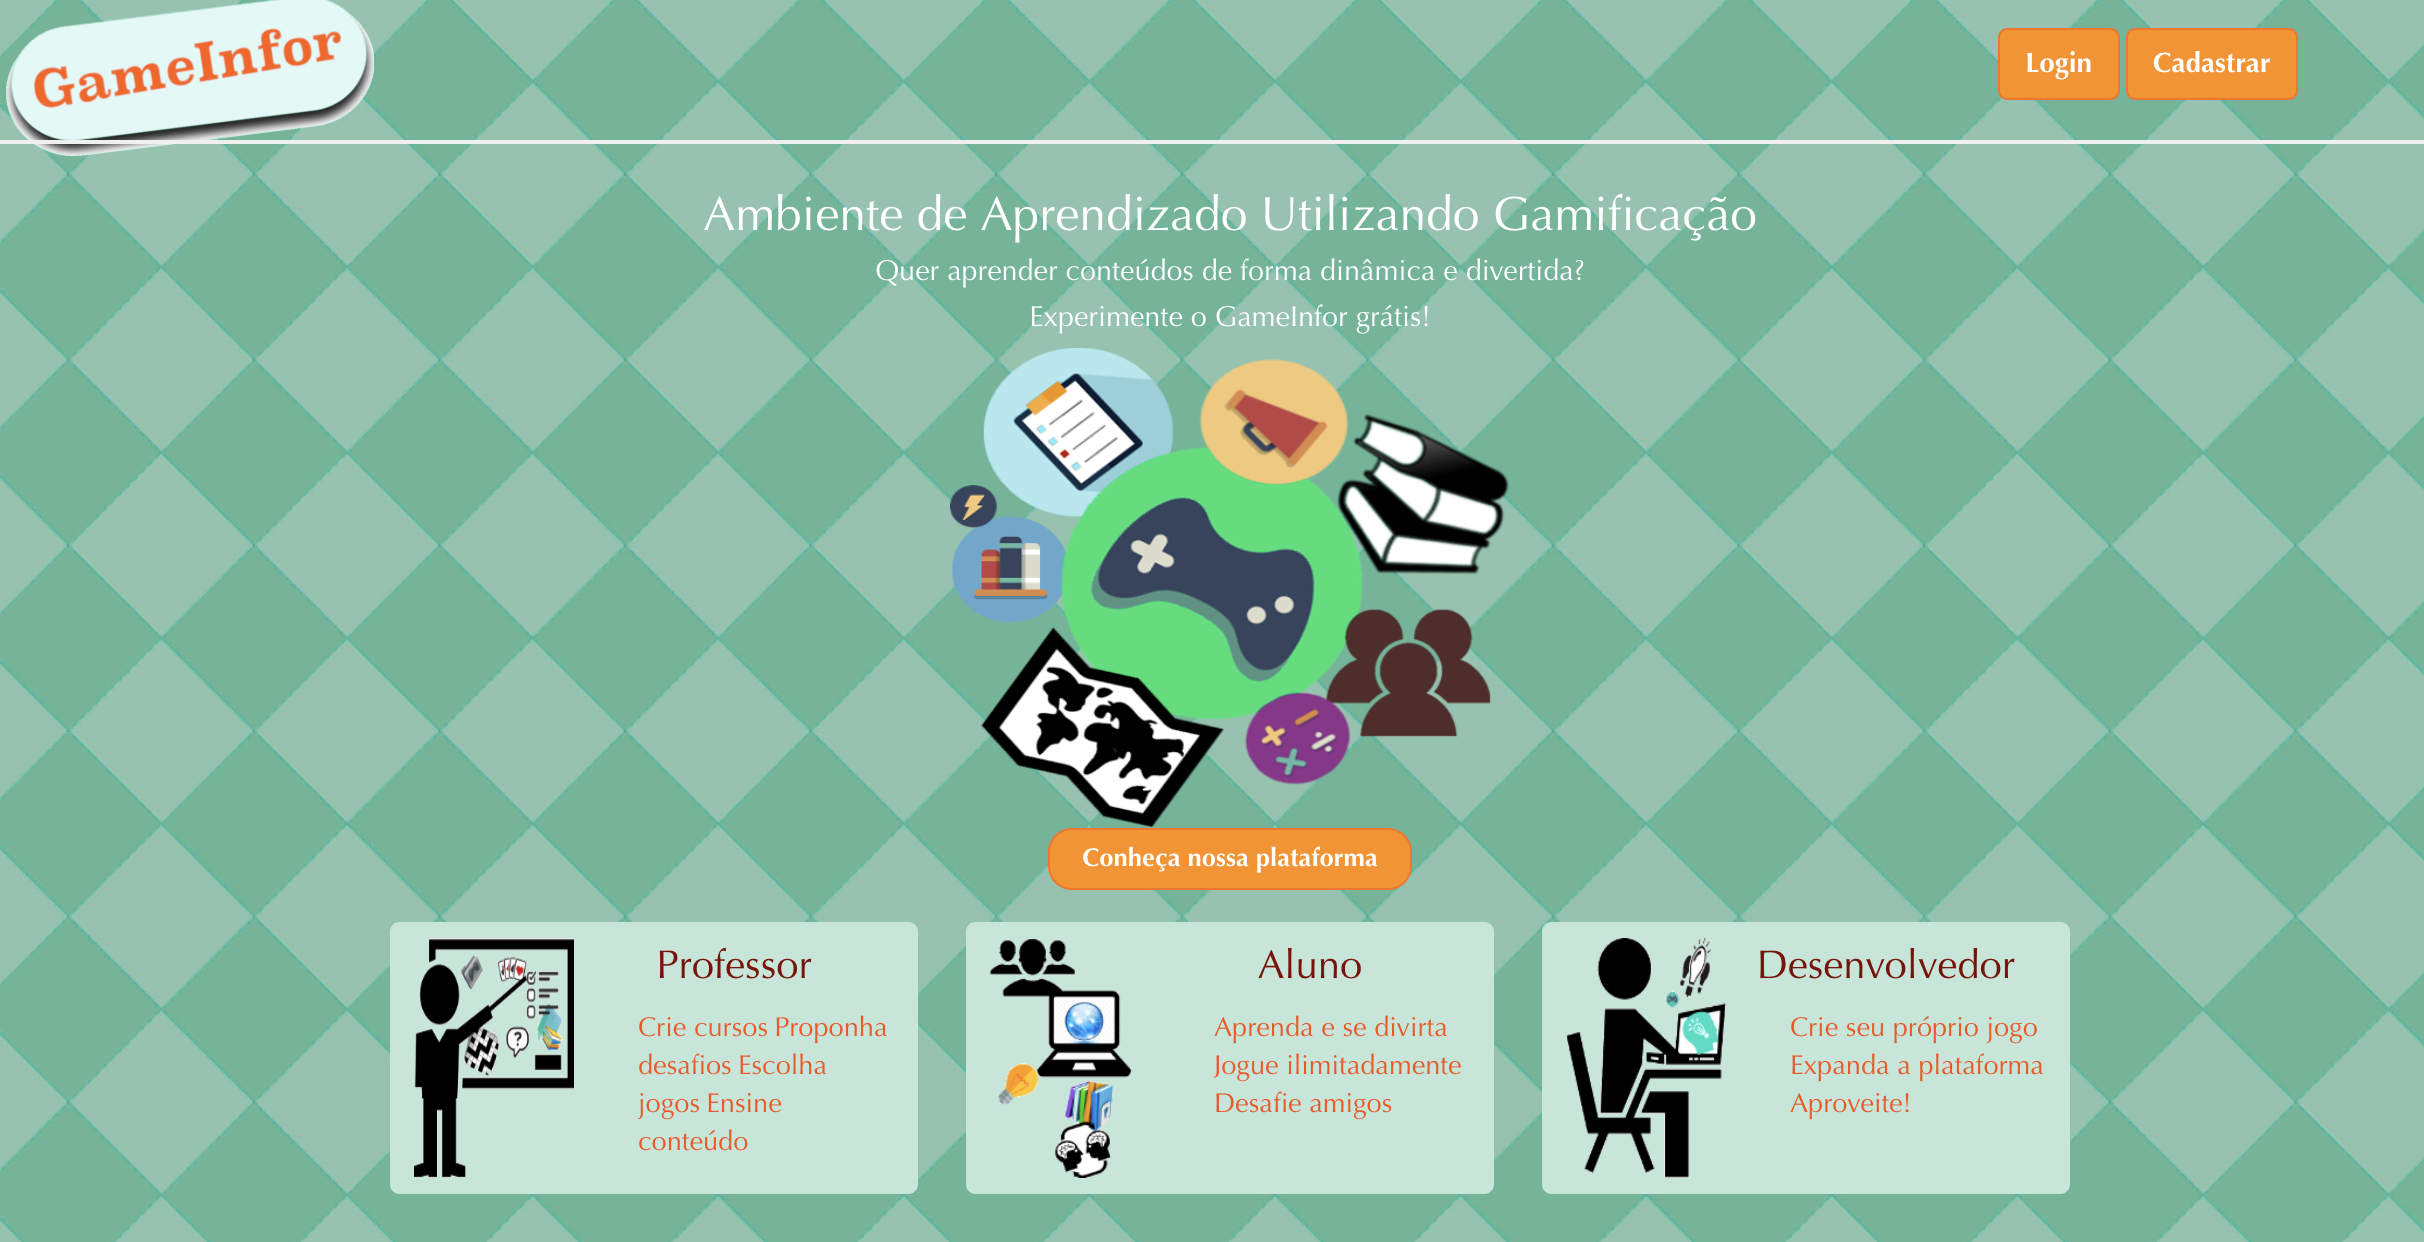
\includegraphics[width=15cm, height=7cm]{images/proposta-img/Figura4-8.png}
  \caption{Tela Inicial}
  \label{fig:Figura4-8}
\end{center}
\end{figure}

\subsection{Login}

Para acessar a plataforma é necessário clicar no botão "Login"  localizado no topo da tela inicial, após realizar esta ação, serão apresentados dois campo para que o usuário informe os dados obrigatórios \figref{fig:Figura4-9} e clique no botão "Login" localizado ao lado do botão "Voltar".

\begin{figure}[h]
\begin{center}
  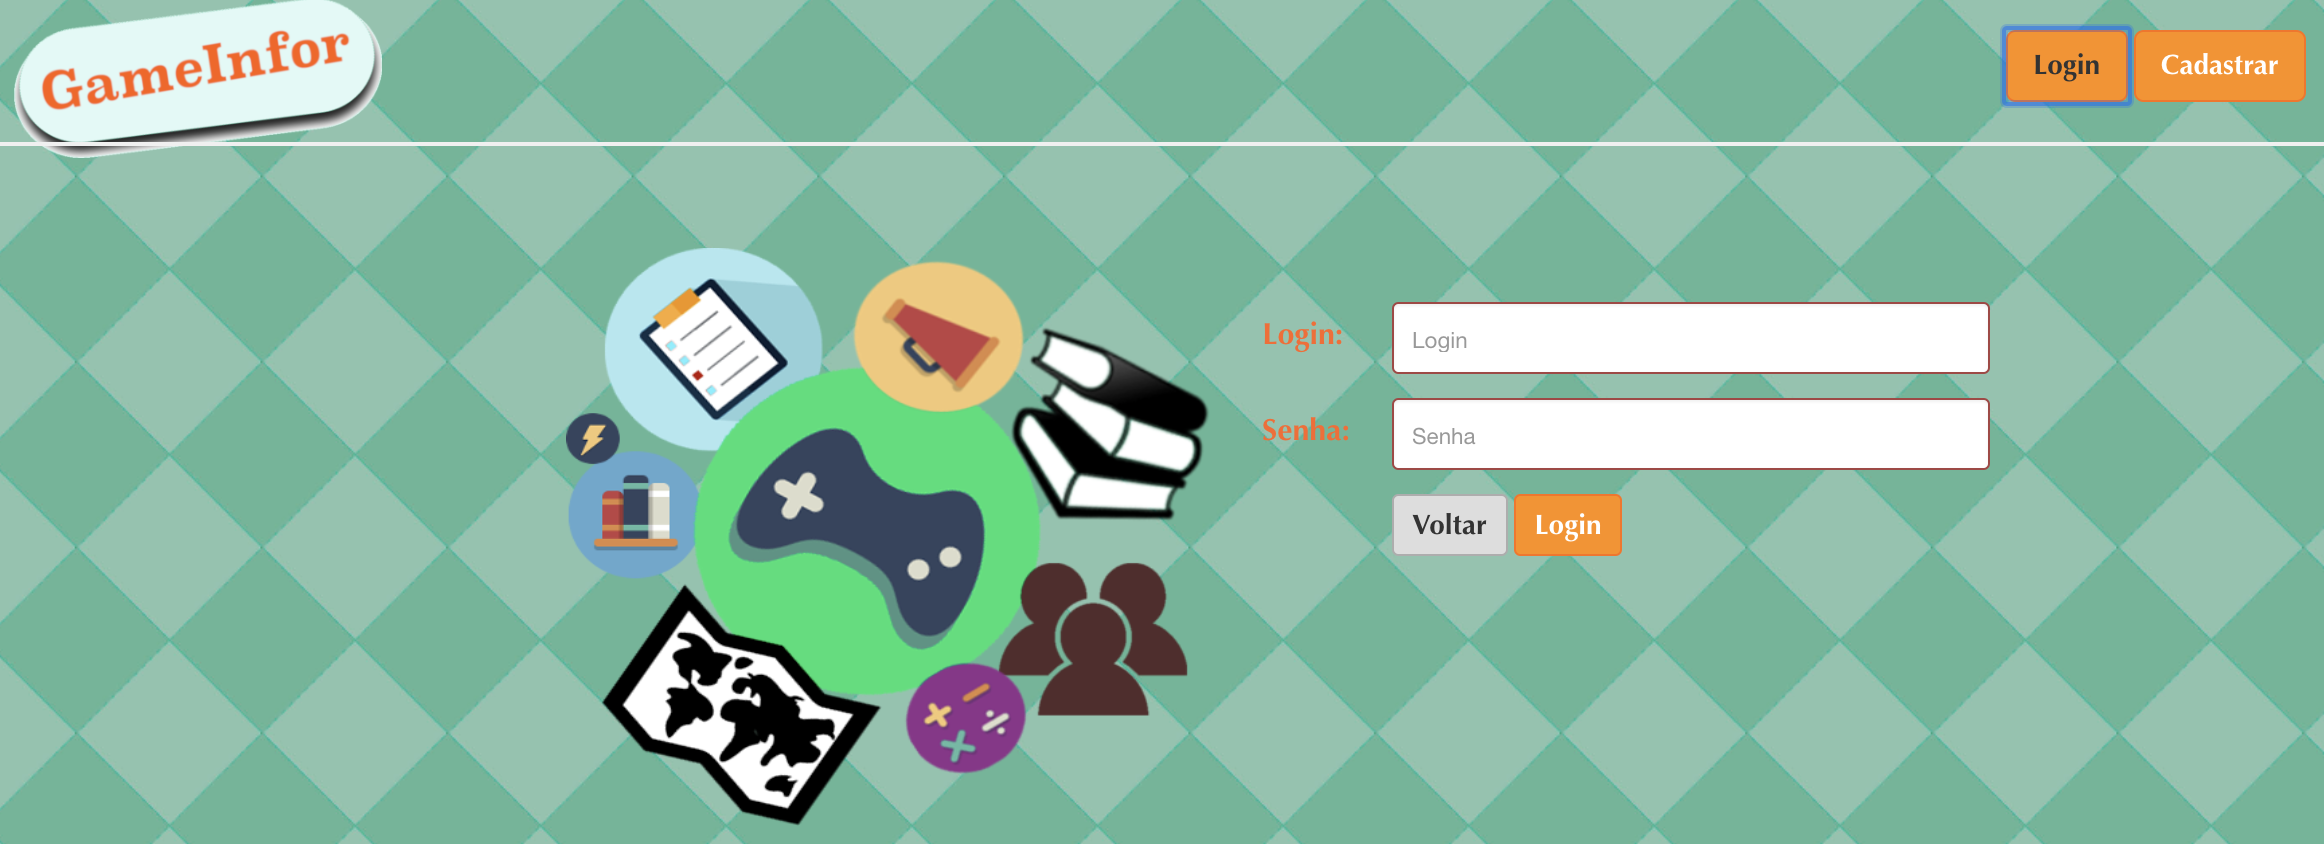
\includegraphics[width=15cm, height=6cm]{images/proposta-img/Figura4-9.png}
  \caption{Tela de Login}
  \label{fig:Figura4-9}
\end{center}
\end{figure}

Seguidamente o sistema identifica o perfil do usuário logado e o direcionará para sua página inicio. Os administradores serão direcionados para a página mostrada na \figref{fig:Figura4-10}, os professores para a \figref{fig:Figura4-11} e os alunos para a \figref{fig:Figura4-12} .


\begin{figure}[H]
  \centering
  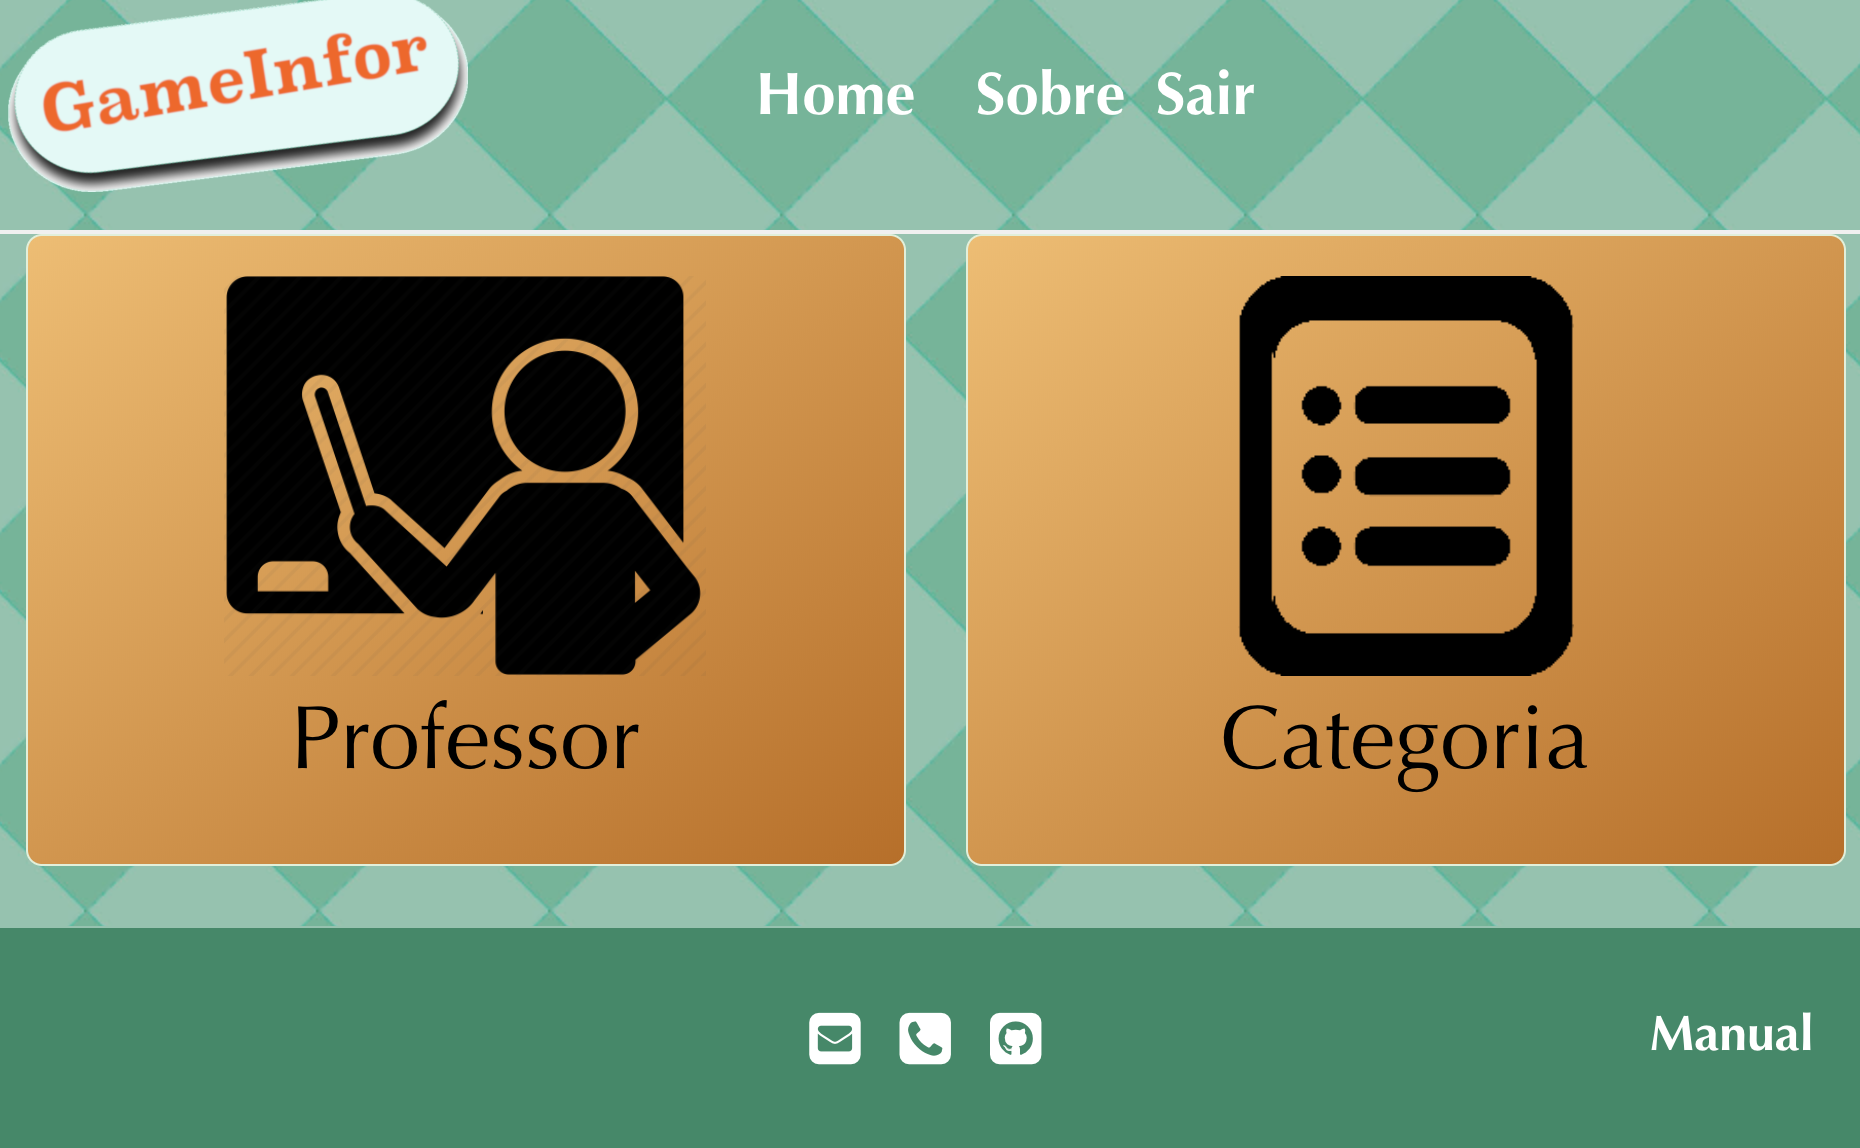
\includegraphics[scale=0.45]{images/proposta-img/Figura4-10.png}
  \caption{Tela Inicial do Administrador}
  \label{fig:Figura4-10}
\end{figure}

\begin{figure}[H]
  \centering
  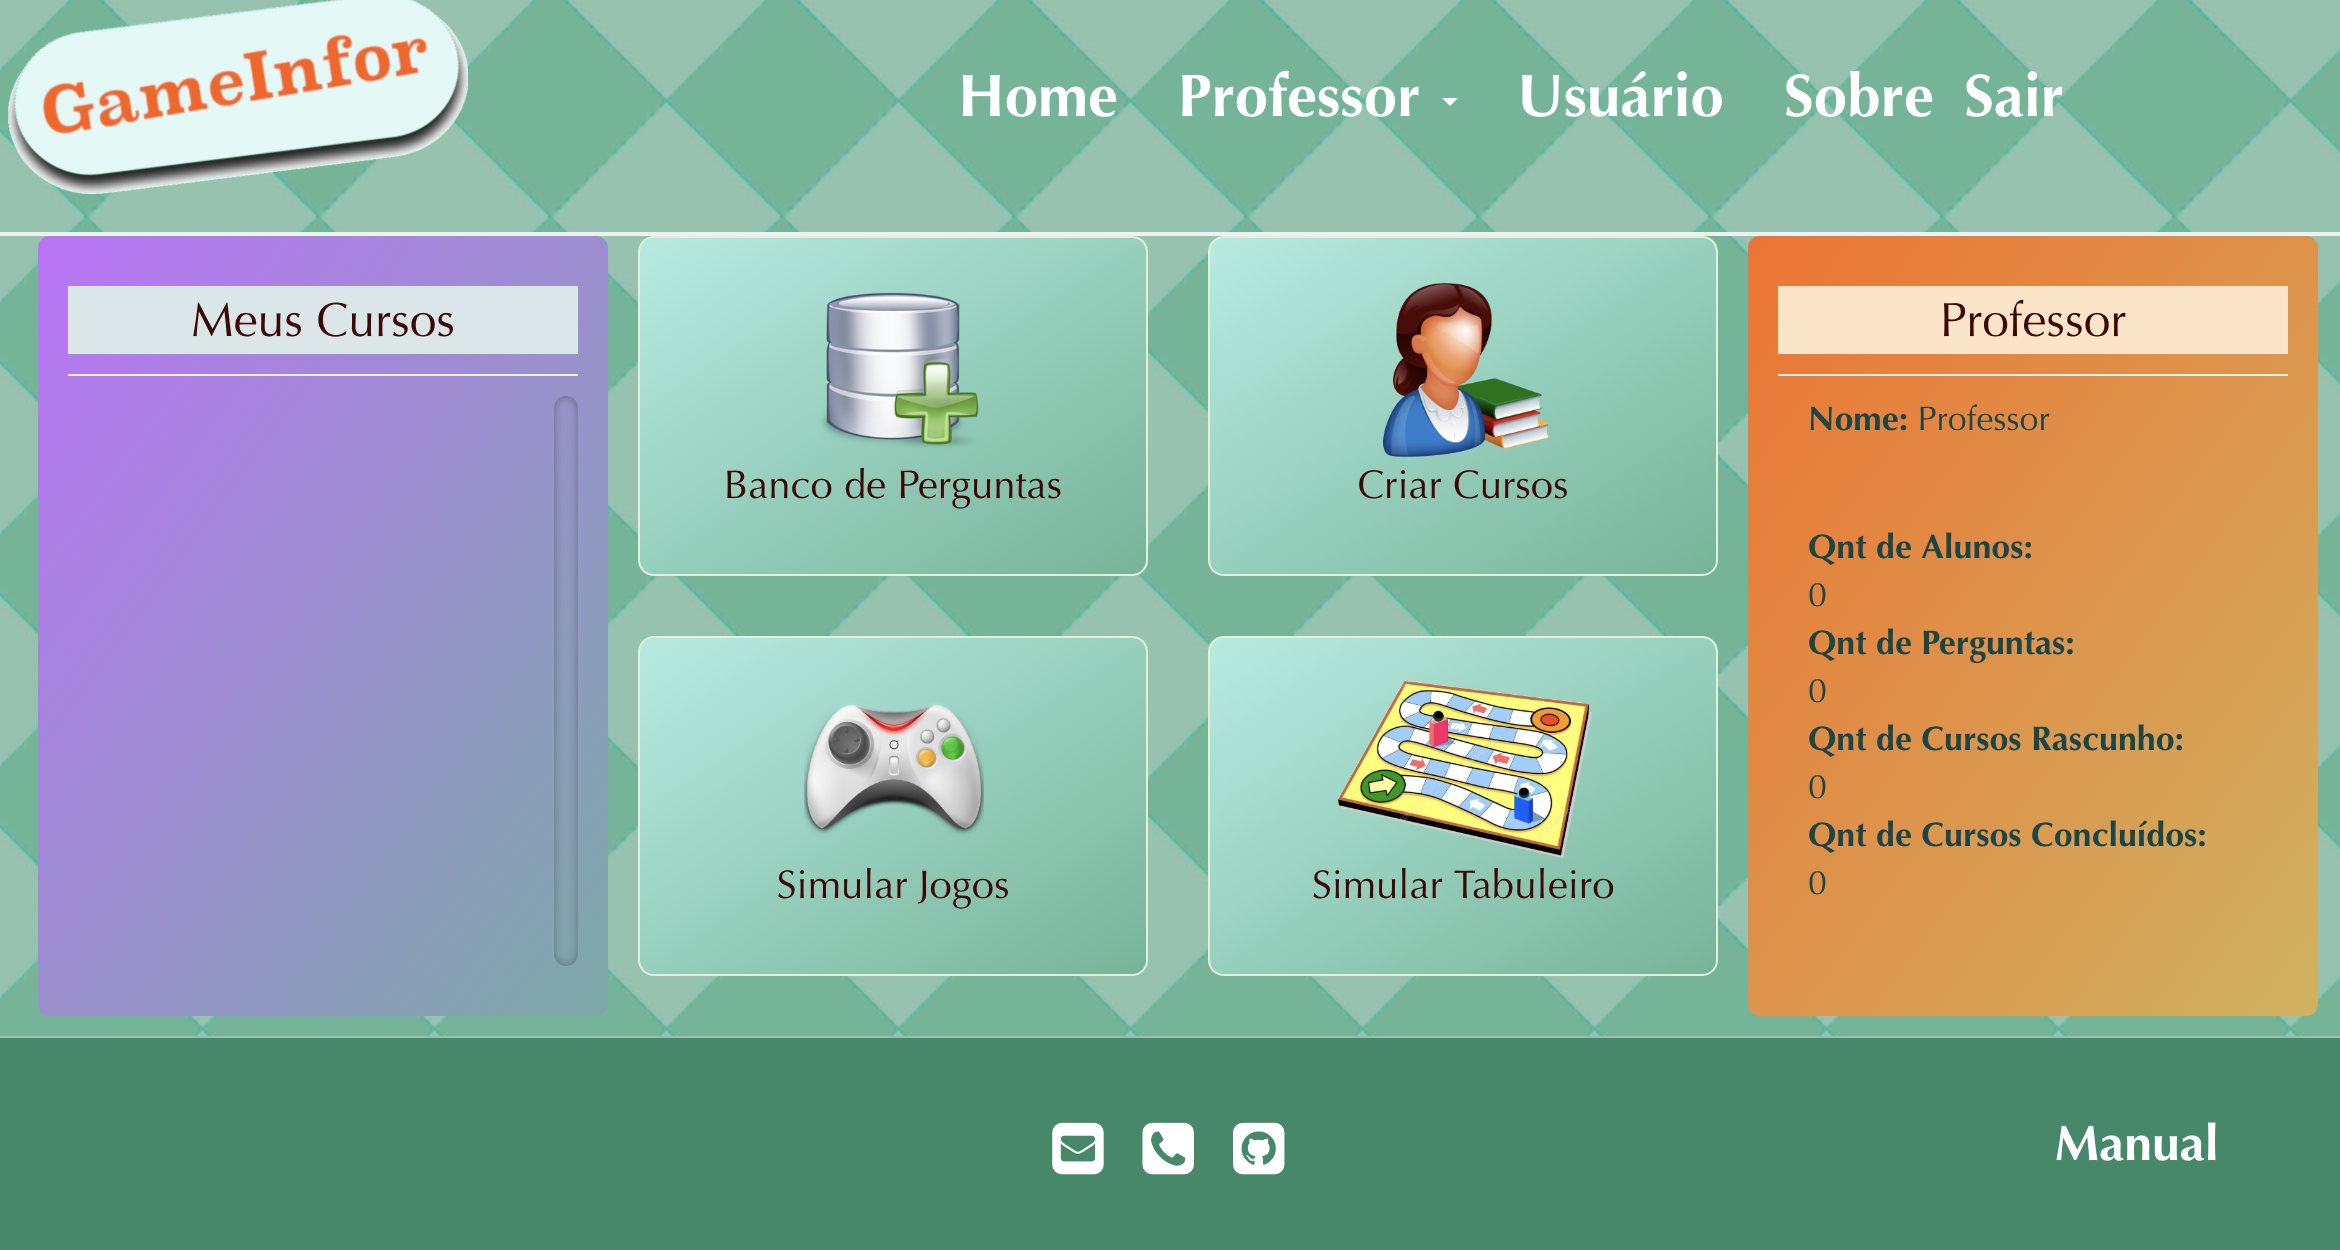
\includegraphics[scale=0.4]{images/proposta-img/Figura4-11.png}
  \caption{Tela Inicial do Professor}
  \label{fig:Figura4-11}
\end{figure}

\begin{figure}[H]
  \centering
  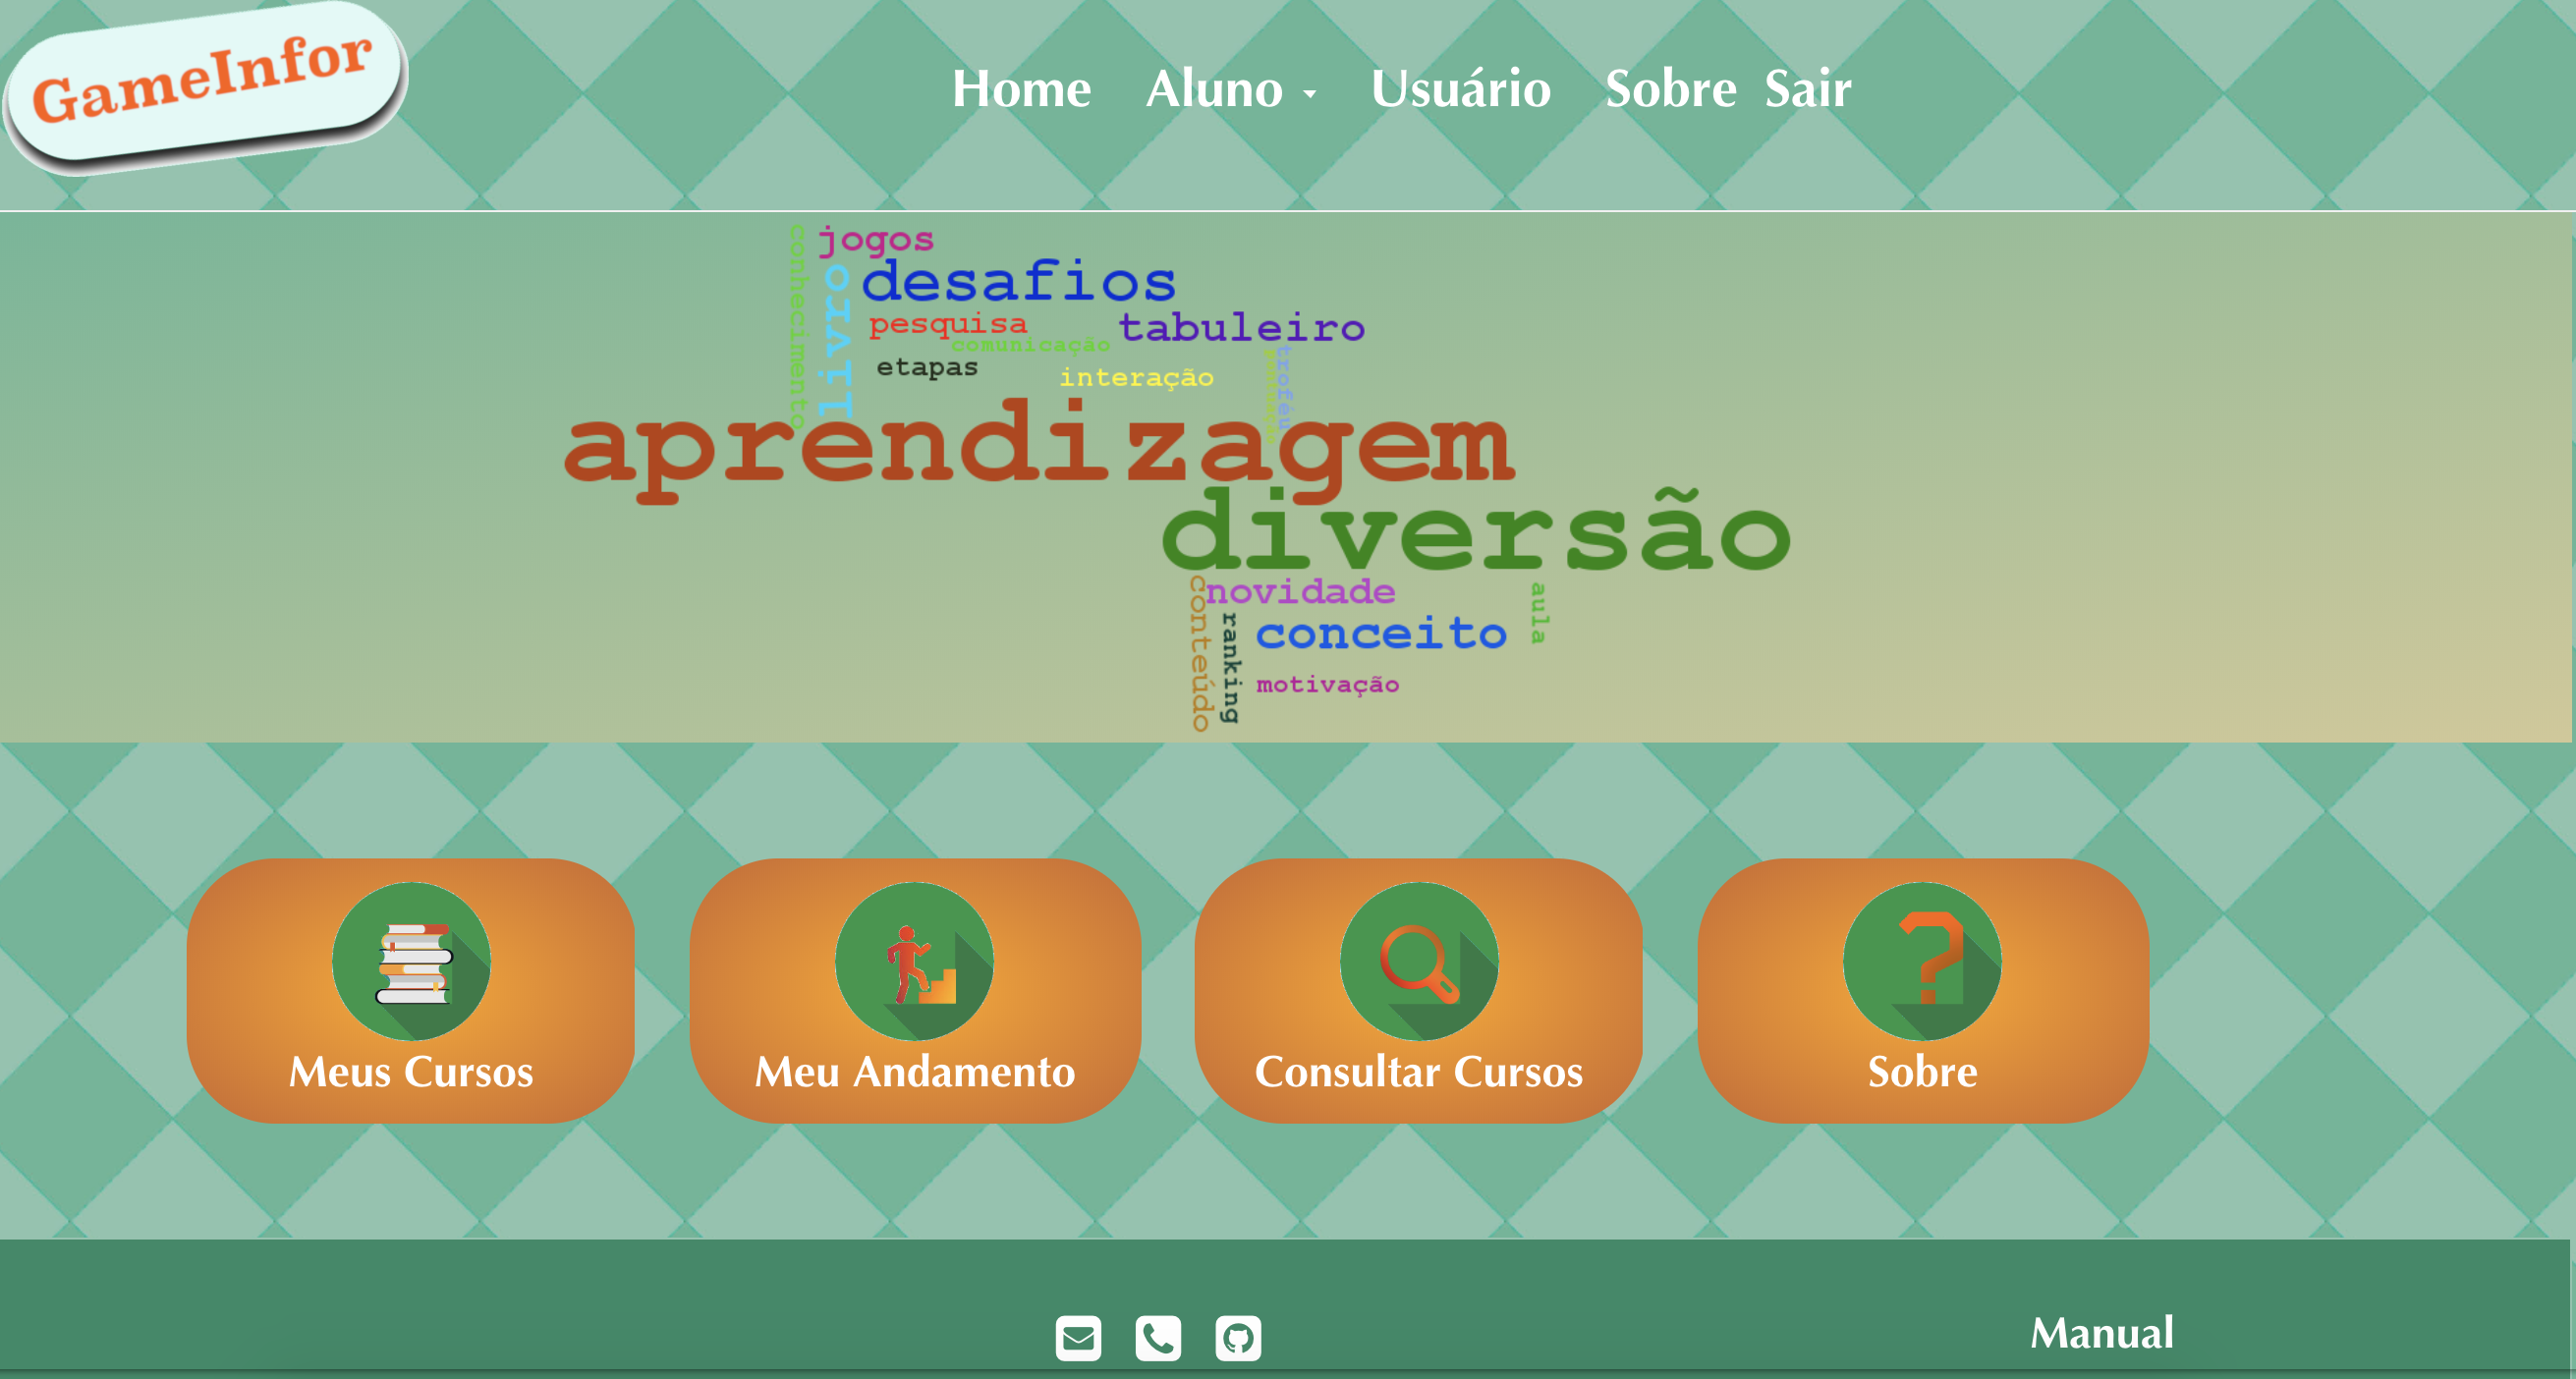
\includegraphics[scale=0.34]{images/proposta-img/Figura4-12.png}
  \caption{Tela Inicial do Aluno}
  \label{fig:Figura4-12}
\end{figure}


\subsection{Editar Dados do Usuário}

Para editar os seus dados pessoais dos professores e dos alunos o usuário pode acessar a aplicação e ir no menu Usuário. Nesta tela existem campos editáveis com  os dados atuais do usuário. Desta forma, a pessoa pode modificar a informação que desejar e apertar o botão salvar.

\begin{figure}[H]
  \centering
  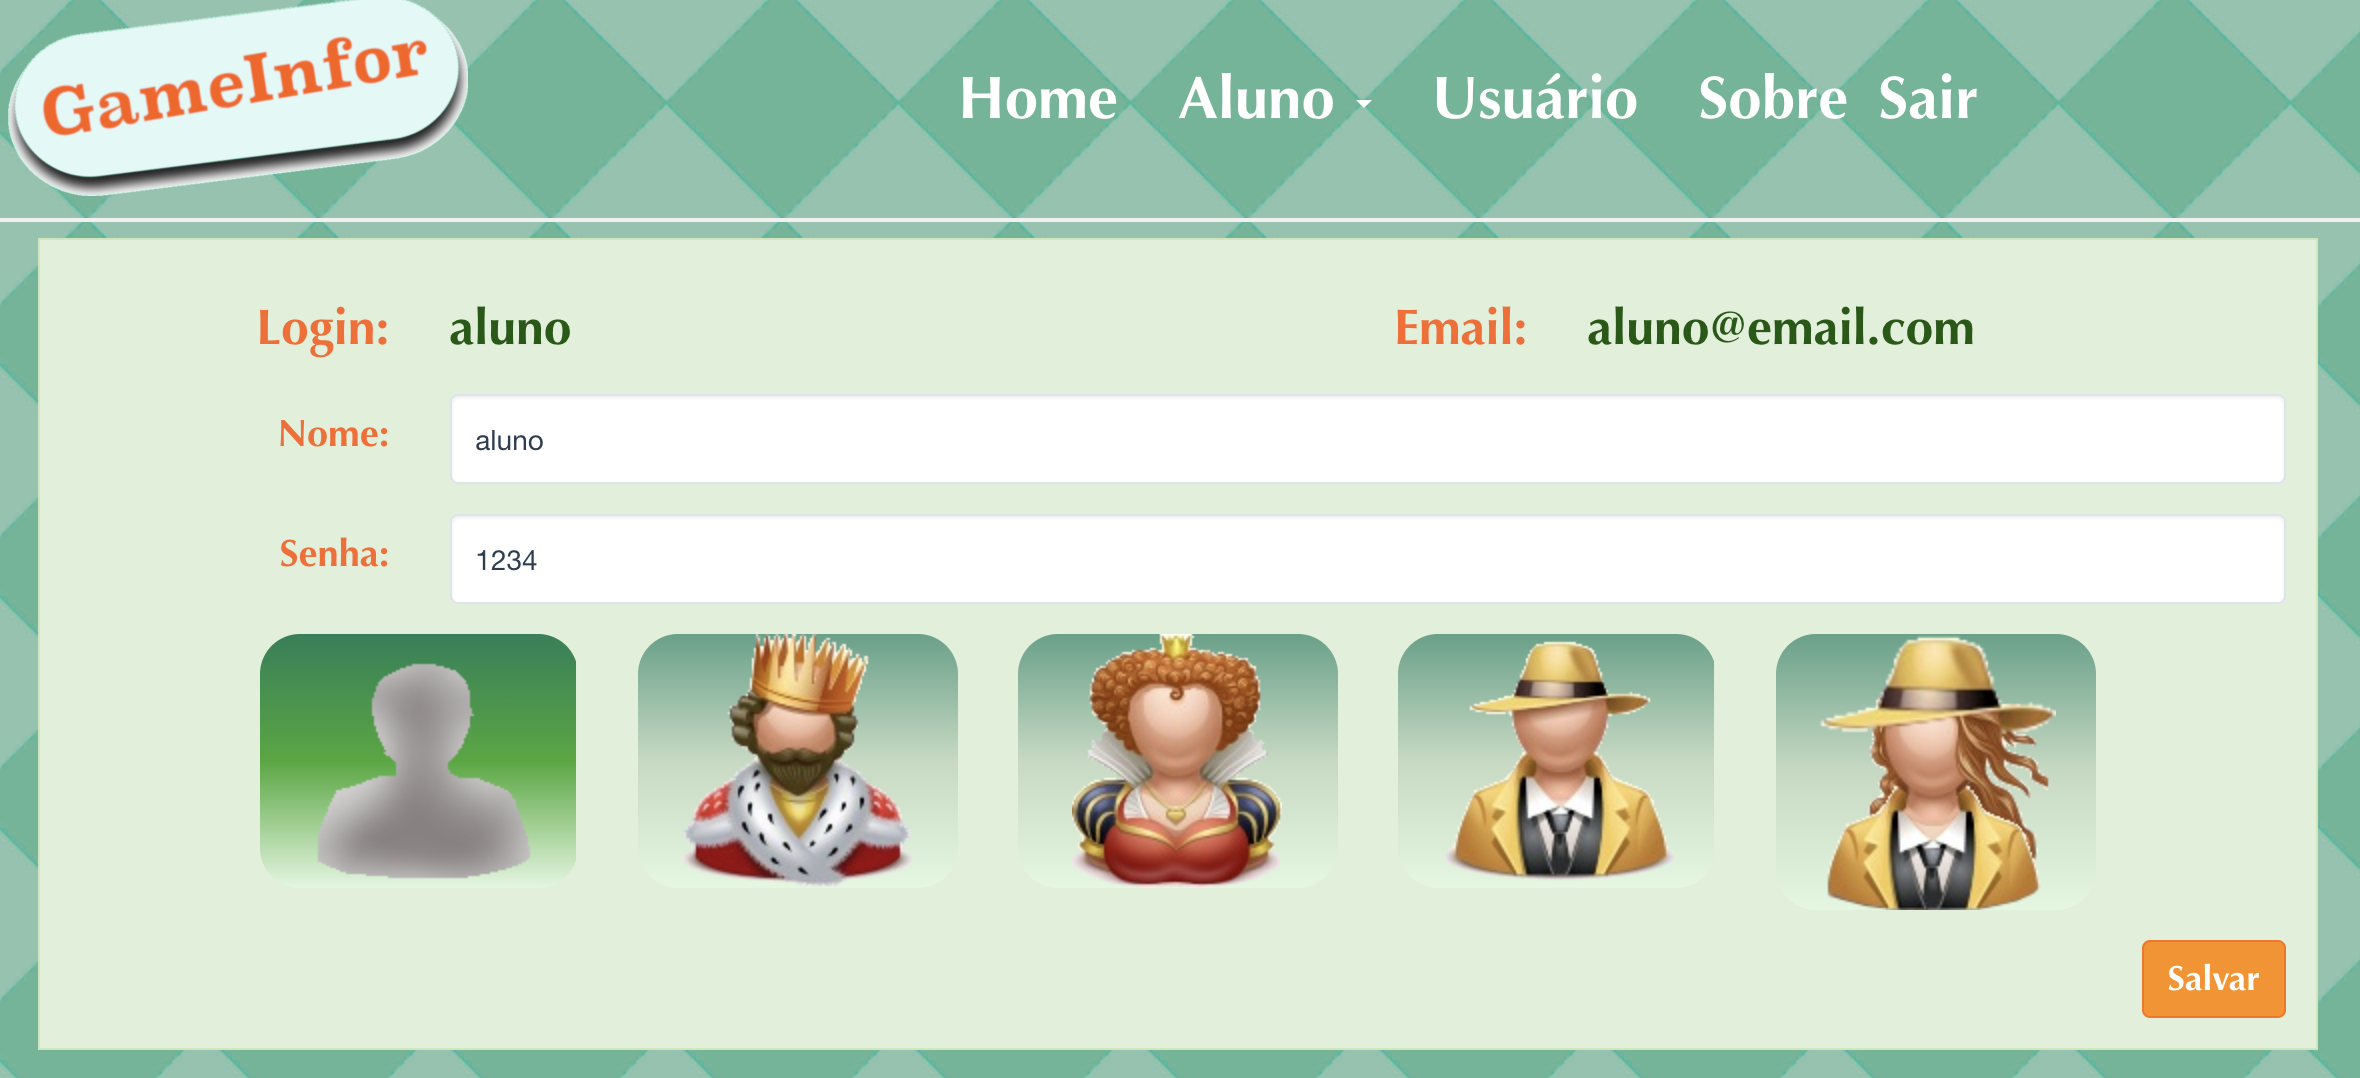
\includegraphics[scale=0.37]{images/proposta-img/Figura4-13.png}
  \caption{Tela de Editar Dados do Usuário}
  \label{fig:Figura4-13}
\end{figure}

\subsection{Tela Sobre}

Com o intuito de conhecer a proposta da plataforma, o usuário pode acessar o menu "Sobre", após o clique a tela apresentará uma breve descrição da missão da plataforma.

\begin{figure}[H]
  \centering
  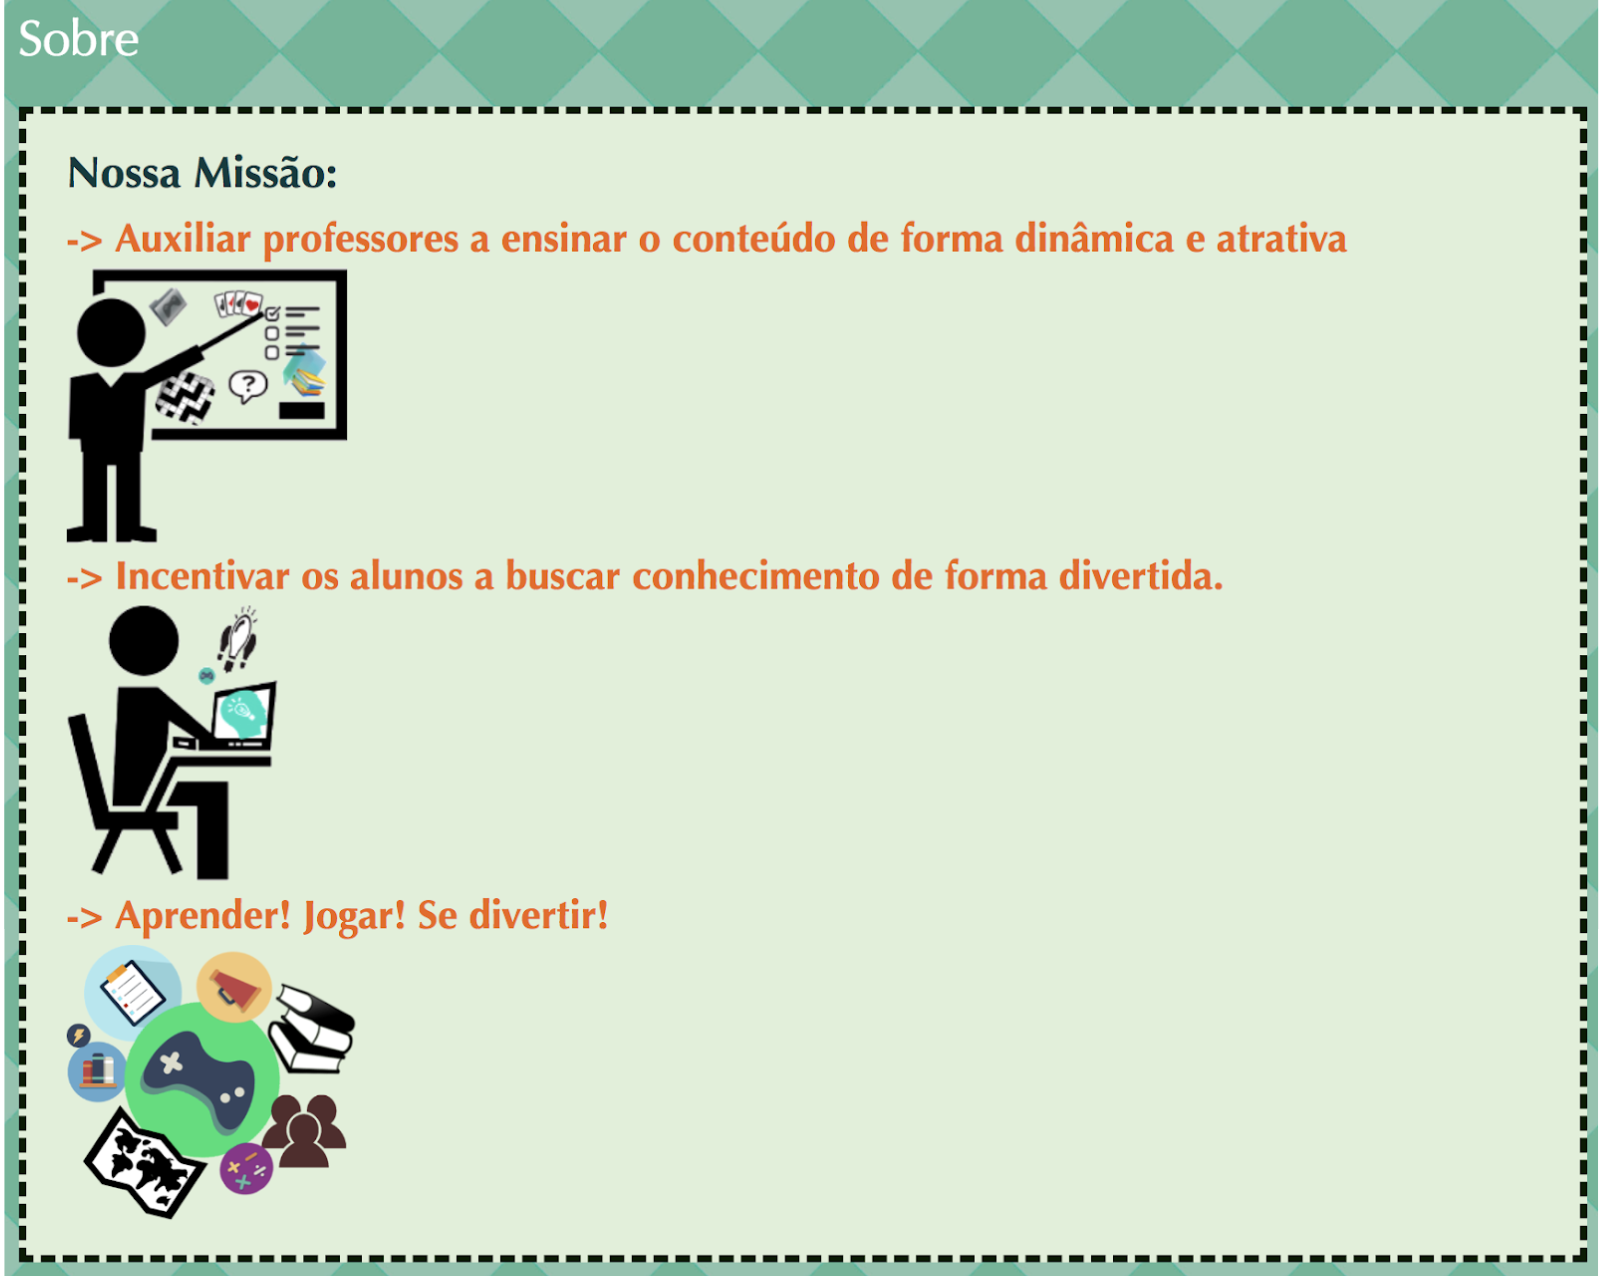
\includegraphics[scale=0.55]{images/proposta-img/Figura4-14.png}
  \caption{Tela Sobre}
  \label{fig:Figura4-14}
\end{figure}


\subsection{Manual}

Com intuito de auxiliar os usuários na utilização da plataforma, foi disponibilizado por intermédio do download um manual de uso para o usuário. O link para baixar o arquivo está no rodapé da página. Vale destacar que existem tem 3 manuais no sistema, e o usuário será direcionado para o manual com as funcionalidades do perfil logado.

\subsection{Funcionalidades do Administrador}

Nesta seção, serão mostradas as funcionalidades disponíveis para um usuário com o perfil de administrador. A pessoa com esse perfil pode manipular as informações dos professores e das categorias da plataforma.
\subsubsection{Dados dos Professor}
O cadastro, edição, exclusão e consulta de professores podem ser efetivadas ao clicar no menu "Professor", ao realizar essa ação o administrador entrará na tela disponível na imagem \figref{fig:Figura4-15}. 

A fim de cadastrar um professor, é necessário clicar no botão "Novo Professor", inserir as informações obrigatória (\figref{fig:Figura4-16}) e clicar no botão "Cadastrar". Após realizar essa ação os dados do professor pode ser consultados, editados e excluídos através da tela mostrada na imagem \figref{fig:Figura4-15}. Para consultar o professor, o administrador pode passar como filtro o nome ou parte do nome do professor e clicar em "Pesquisar", após a apresentação da lista de resultados o usuário pode excluir ou editar um professor. Para excluir é necessário clicar no  "X" ao lado do nome do professor listado, e confirmar a ação. Se desejar editar o usuário pode clicar no lápis, que o direciona para a mesma tela de cadastro porém com os dados preenchidos, ao administrador basta editar o campo desejado e salvar.

\begin{figure}[H]
  \centering
  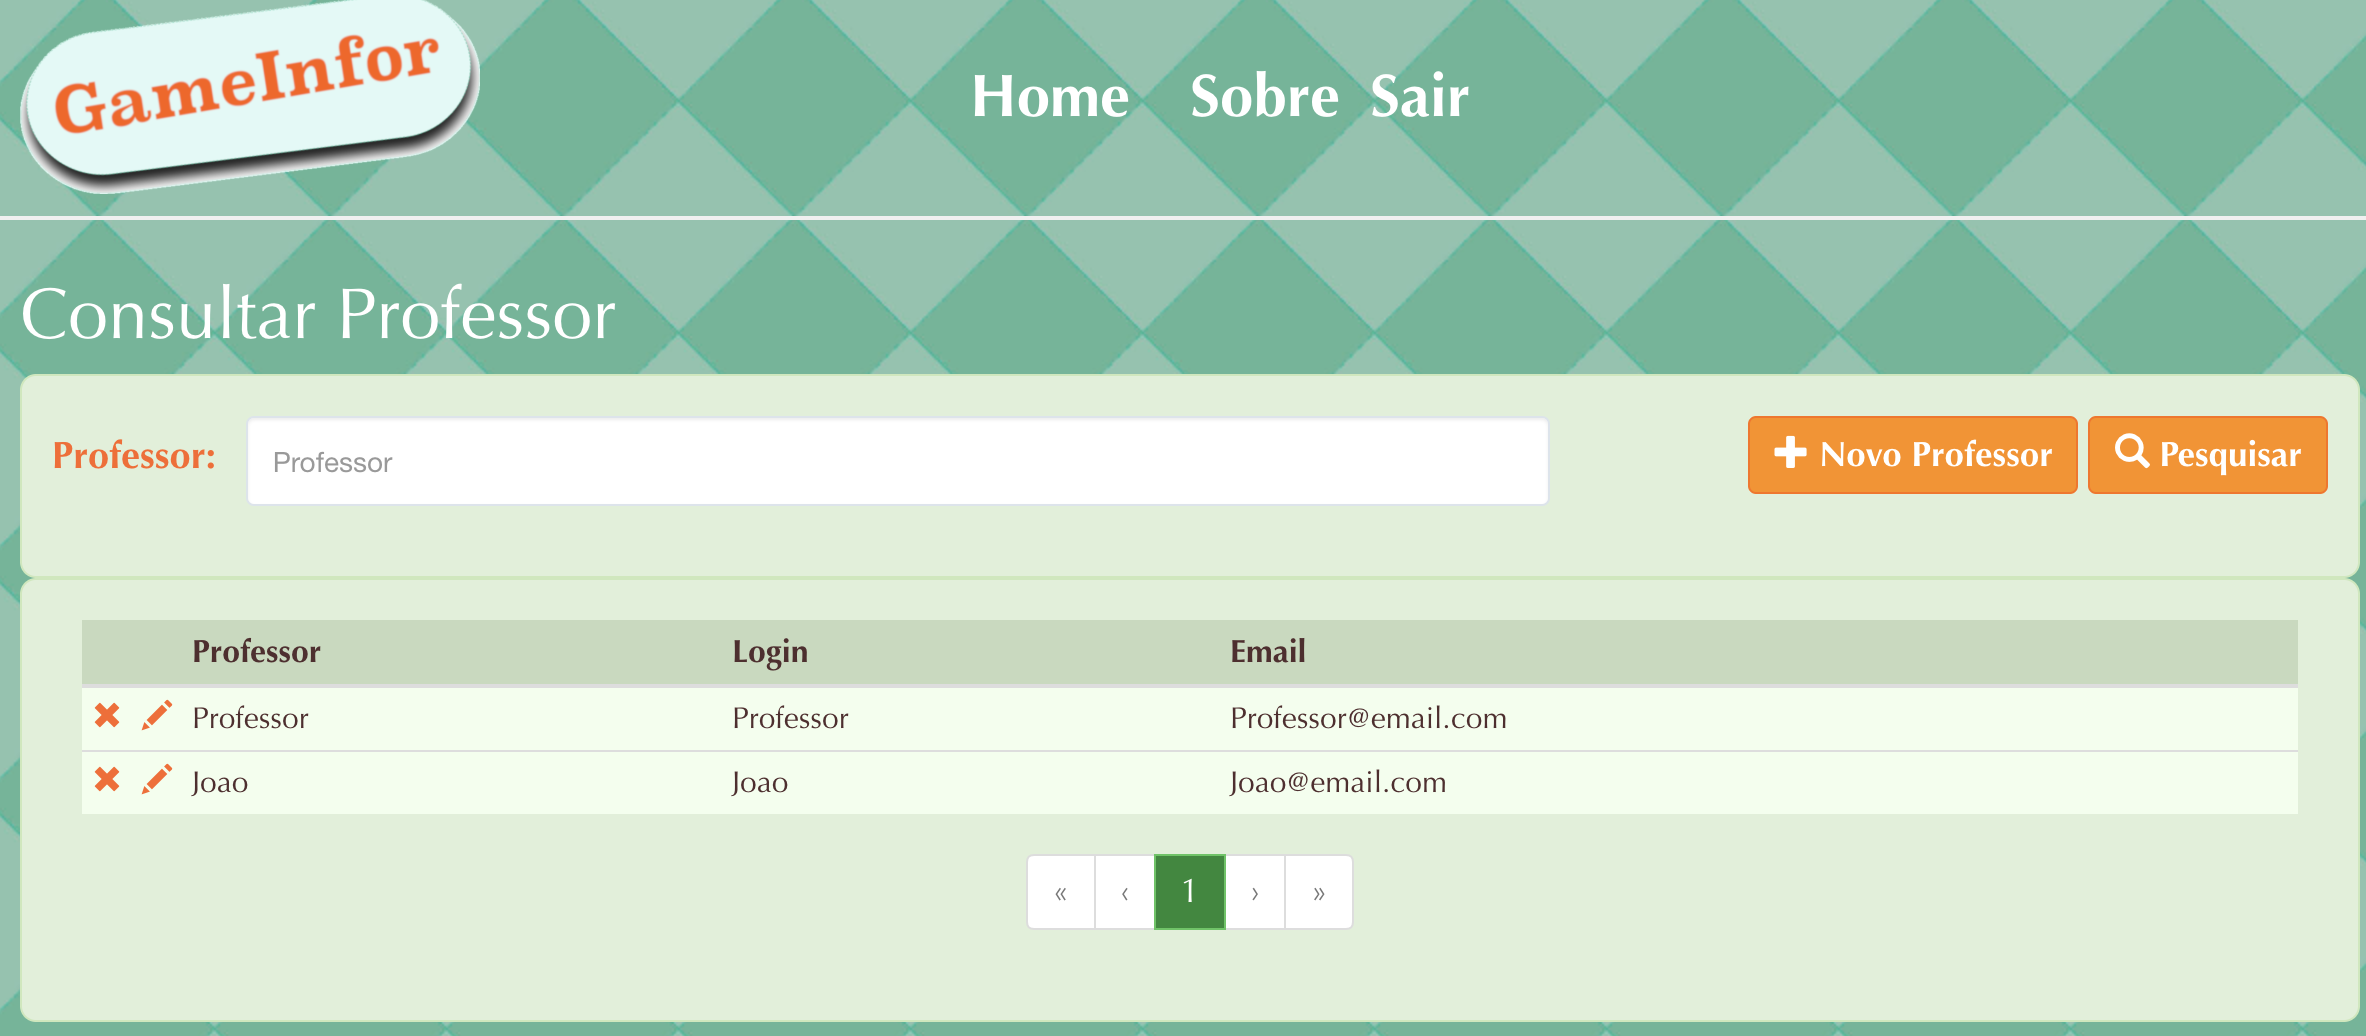
\includegraphics[scale=0.4]{images/proposta-img/Figura4-15.png}
  \caption{Tela de Consultar Professor}
  \label{fig:Figura4-15}
\end{figure}

\begin{figure}[H]
  \centering
  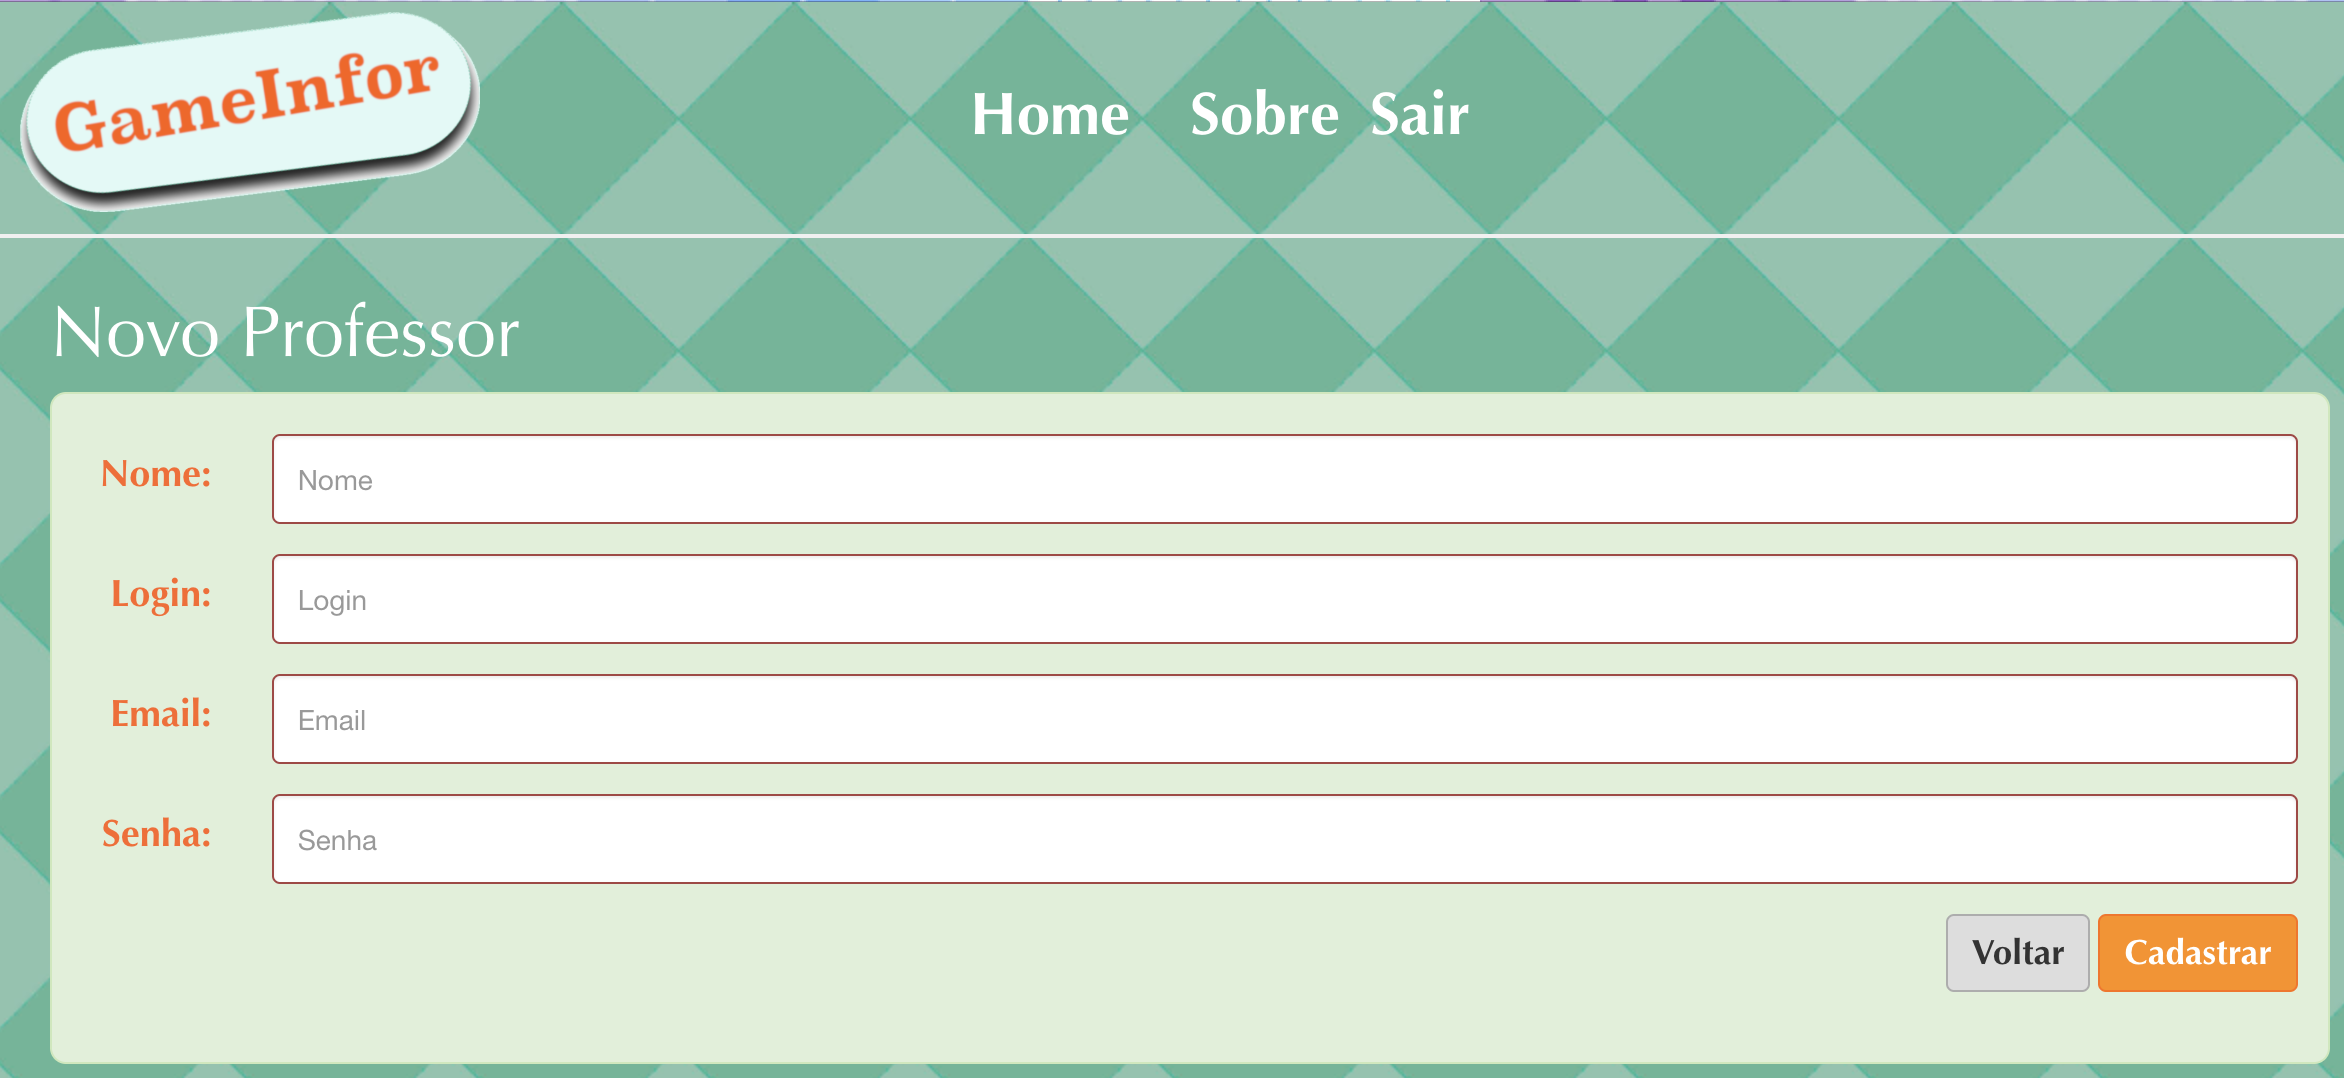
\includegraphics[scale=0.4]{images/proposta-img/Figura4-16.png}
  \caption{Tela de Cadastrar Professor}
  \label{fig:Figura4-16}
\end{figure}
\subsubsection{Dados das Categoria}
Ao acessar o menu “Categoria” o administrador pode cadastrar, editar, excluir e consultar as categorias existentes na plataforma, ao realizar essa ação o administrador entrará na tela disponível \figref{fig:Figura4-17}. 

Para criar uma nova categoria, é necessário clicar no botão "Nova Categoria", informar o nome e clicar no em"Cadastrar". Após realizar essa ação as categorias podem ser consultados, editados e excluídos através da tela mostrada na figura \figref{fig:Figura4-18}. A consulta pode ser realizada através do botão "Pesquisar", após a apresentação da lista de resultados o usuário pode excluir ou editar uma categoria.

\begin{figure}[H]
  \centering
  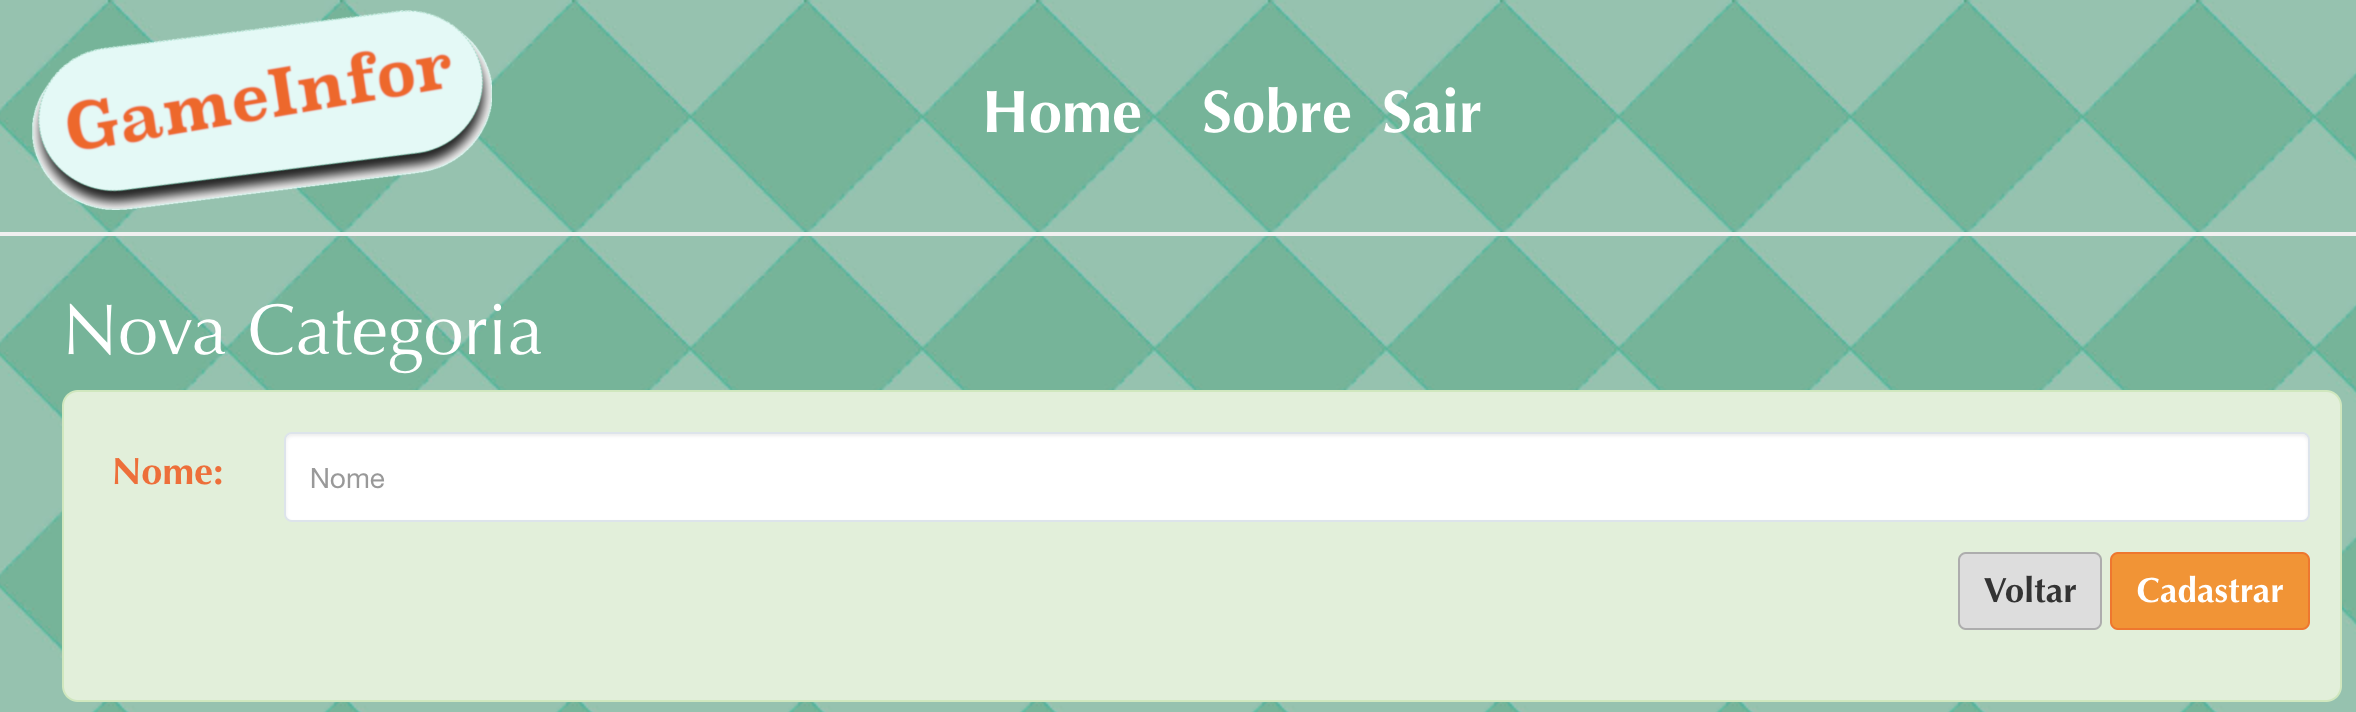
\includegraphics[scale=0.4]{images/proposta-img/Figura4-17.png}
  \caption{Tela de Consultar Categoria}
  \label{fig:Figura4-17}
\end{figure}

\begin{figure}[H]
  \centering
  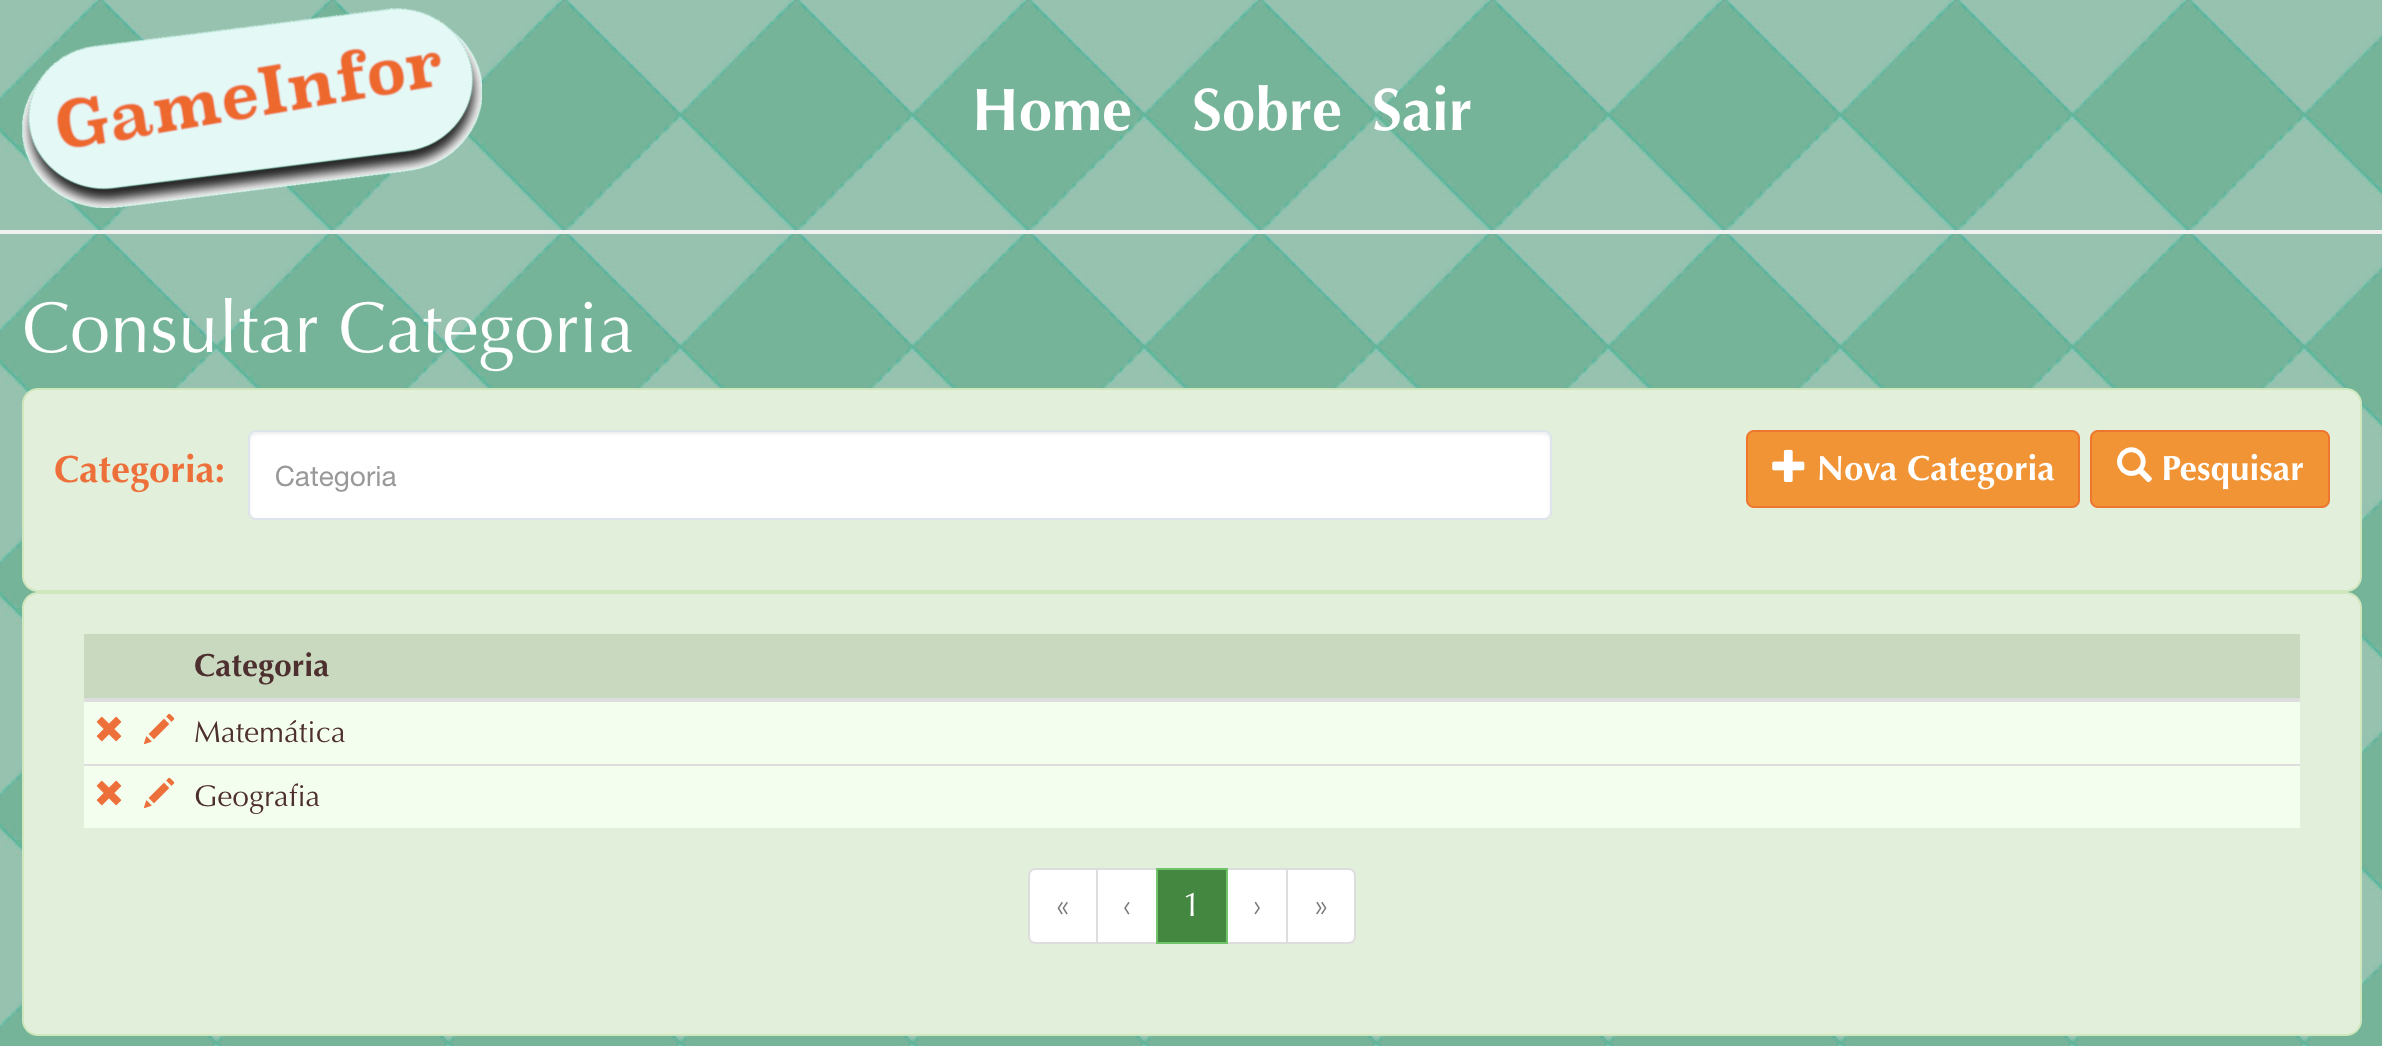
\includegraphics[scale=0.4]{images/proposta-img/Figura4-18.png}
  \caption{Tela de Cadastrar Categoria}
  \label{fig:Figura4-18}
\end{figure}

\subsection{Funcionalidades do Professor}
Nesta seção, serão mostradas as funcionalidades disponíveis para um usuário com o perfil de professor. A pessoa com esse perfil pode manipular as informações dos professores e das categorias da plataforma.
\subsubsection{Dados das Perguntas}

Ao acessar o menu “Pergunta” o administrador pode cadastrar, editar, excluir e consultar as categorias existentes na plataforma, ao realizar essa ação o administrador entrará na tela disponível na \figref{fig:Figura4-20}. 

Para criar uma nova pergunta, é necessário clicar no botão "Nova Pergunta" \figref{fig:Figura4-19}, preencher os campos e clicar no em"Cadastrar", ao professor é dada a opção de criar perguntas múltiplas escolhas ou perguntas de completar lacunas, além disso é possível escolher o tempo que o aluno terá para responder a pergunta, a categoria da pergunta e o nível de dificuldade. Se desejar, o professor pode inserir um anexo antes de salvar.

A consulta, edição e exclusão devem ser realizadas por intermédio da tela mostrada na \figref{fig:Figura4-20}.

\begin{figure}[H]
  \centering
  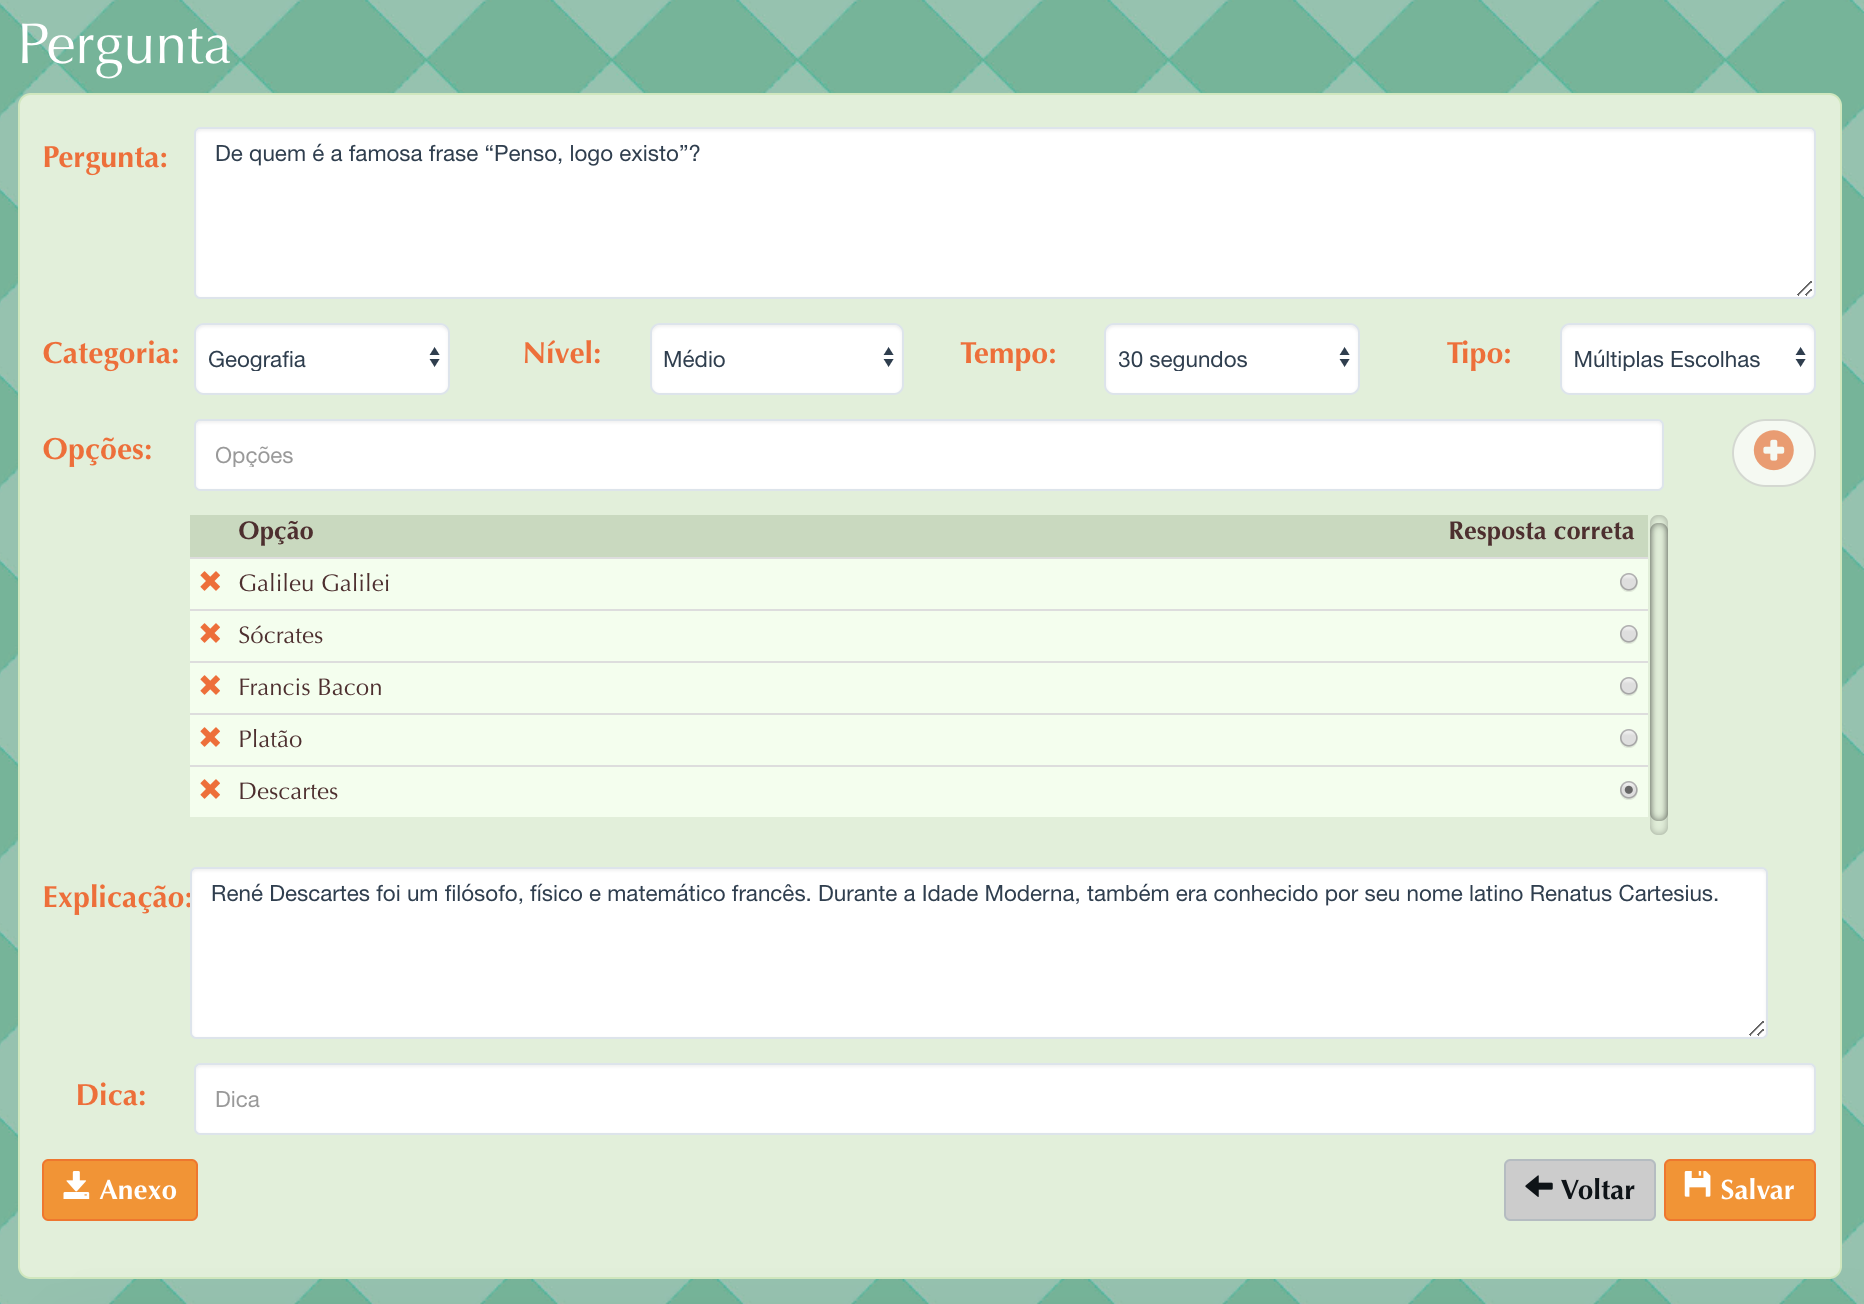
\includegraphics[scale=0.4]{images/proposta-img/Figura4-19.png}
  \caption{Tela de Consultar Perguntas}
  \label{fig:Figura4-19}
\end{figure}

\begin{figure}[H]
  \centering
  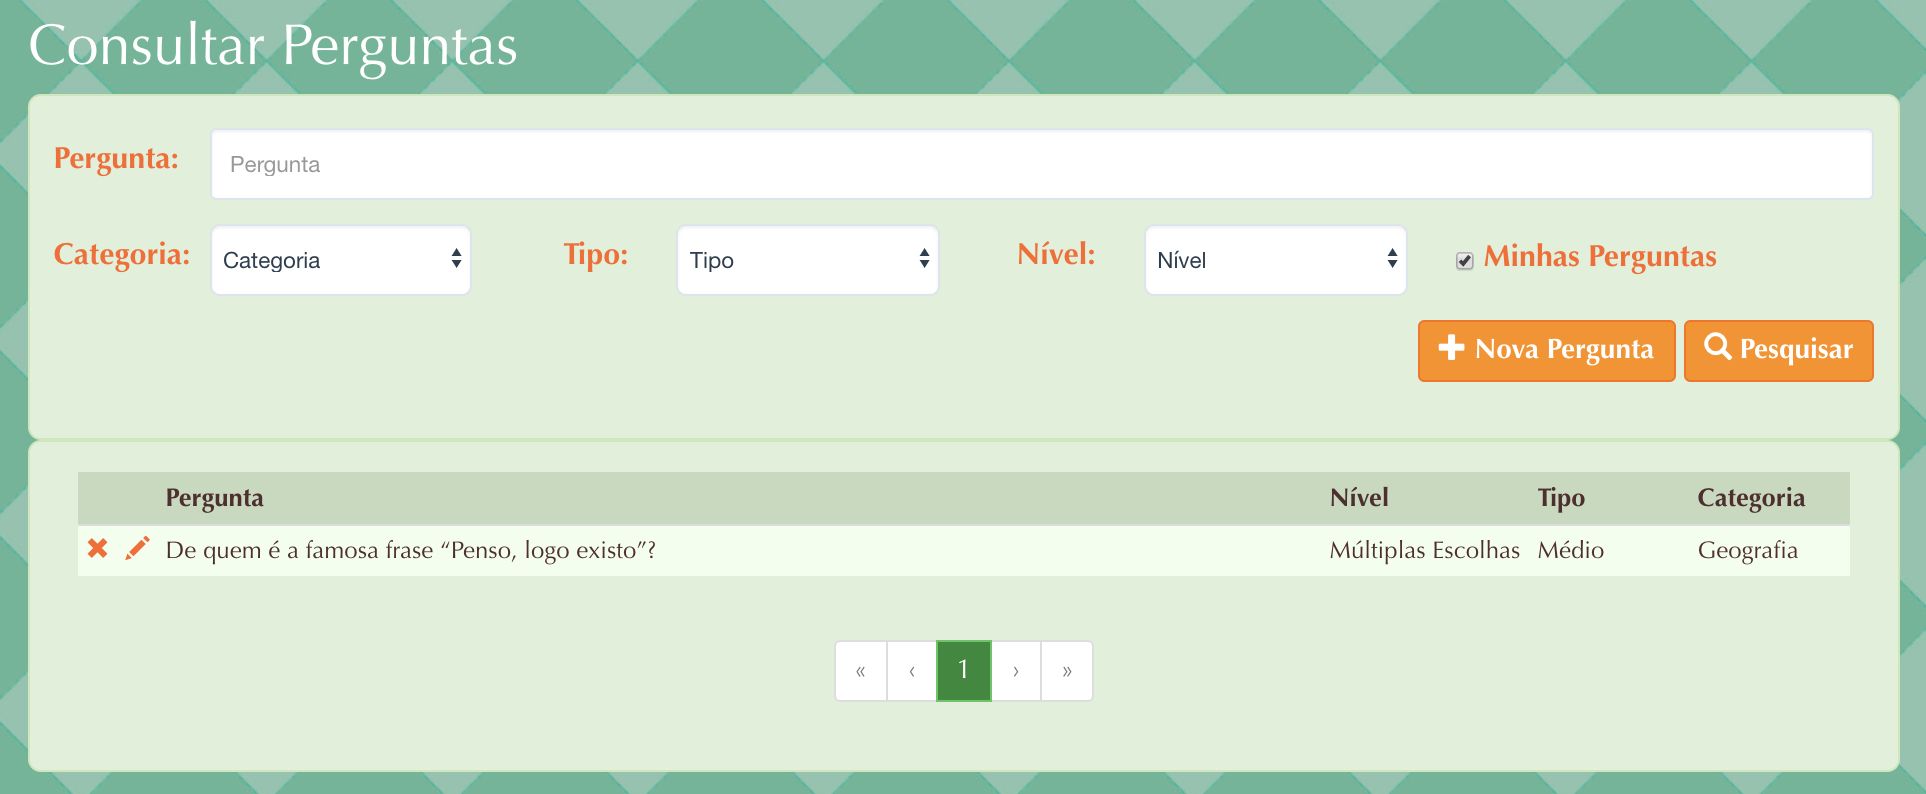
\includegraphics[scale=0.4]{images/proposta-img/Figura4-20.png}
  \caption{Tela de Cadastrar Perguntas}
  \label{fig:Figura4-20}
\end{figure}

\subsubsection{Simulador de Jogo}
No momento em que o professor cria um curso, ele pode selecionar quantas etapas desejar, para cada etapa o aluno deverá ganhar um jogo de perguntas para avançar. Com o intuito de auxiliar os professores, foi disponibilizada a tela \figref{fig:Figura4-21} que pode ser acessada ao clicar no menu Professor e dentro dele selecionar a opção “Jogos”. Está tela contém a simulação de todos os jogos disponíveis na plataforma, até o momento a plataforma tem 5 jogos disponíveis: quiz, forca, aposta, caça palavras e jogo da velha. 
\begin{figure}[H]
  \centering
  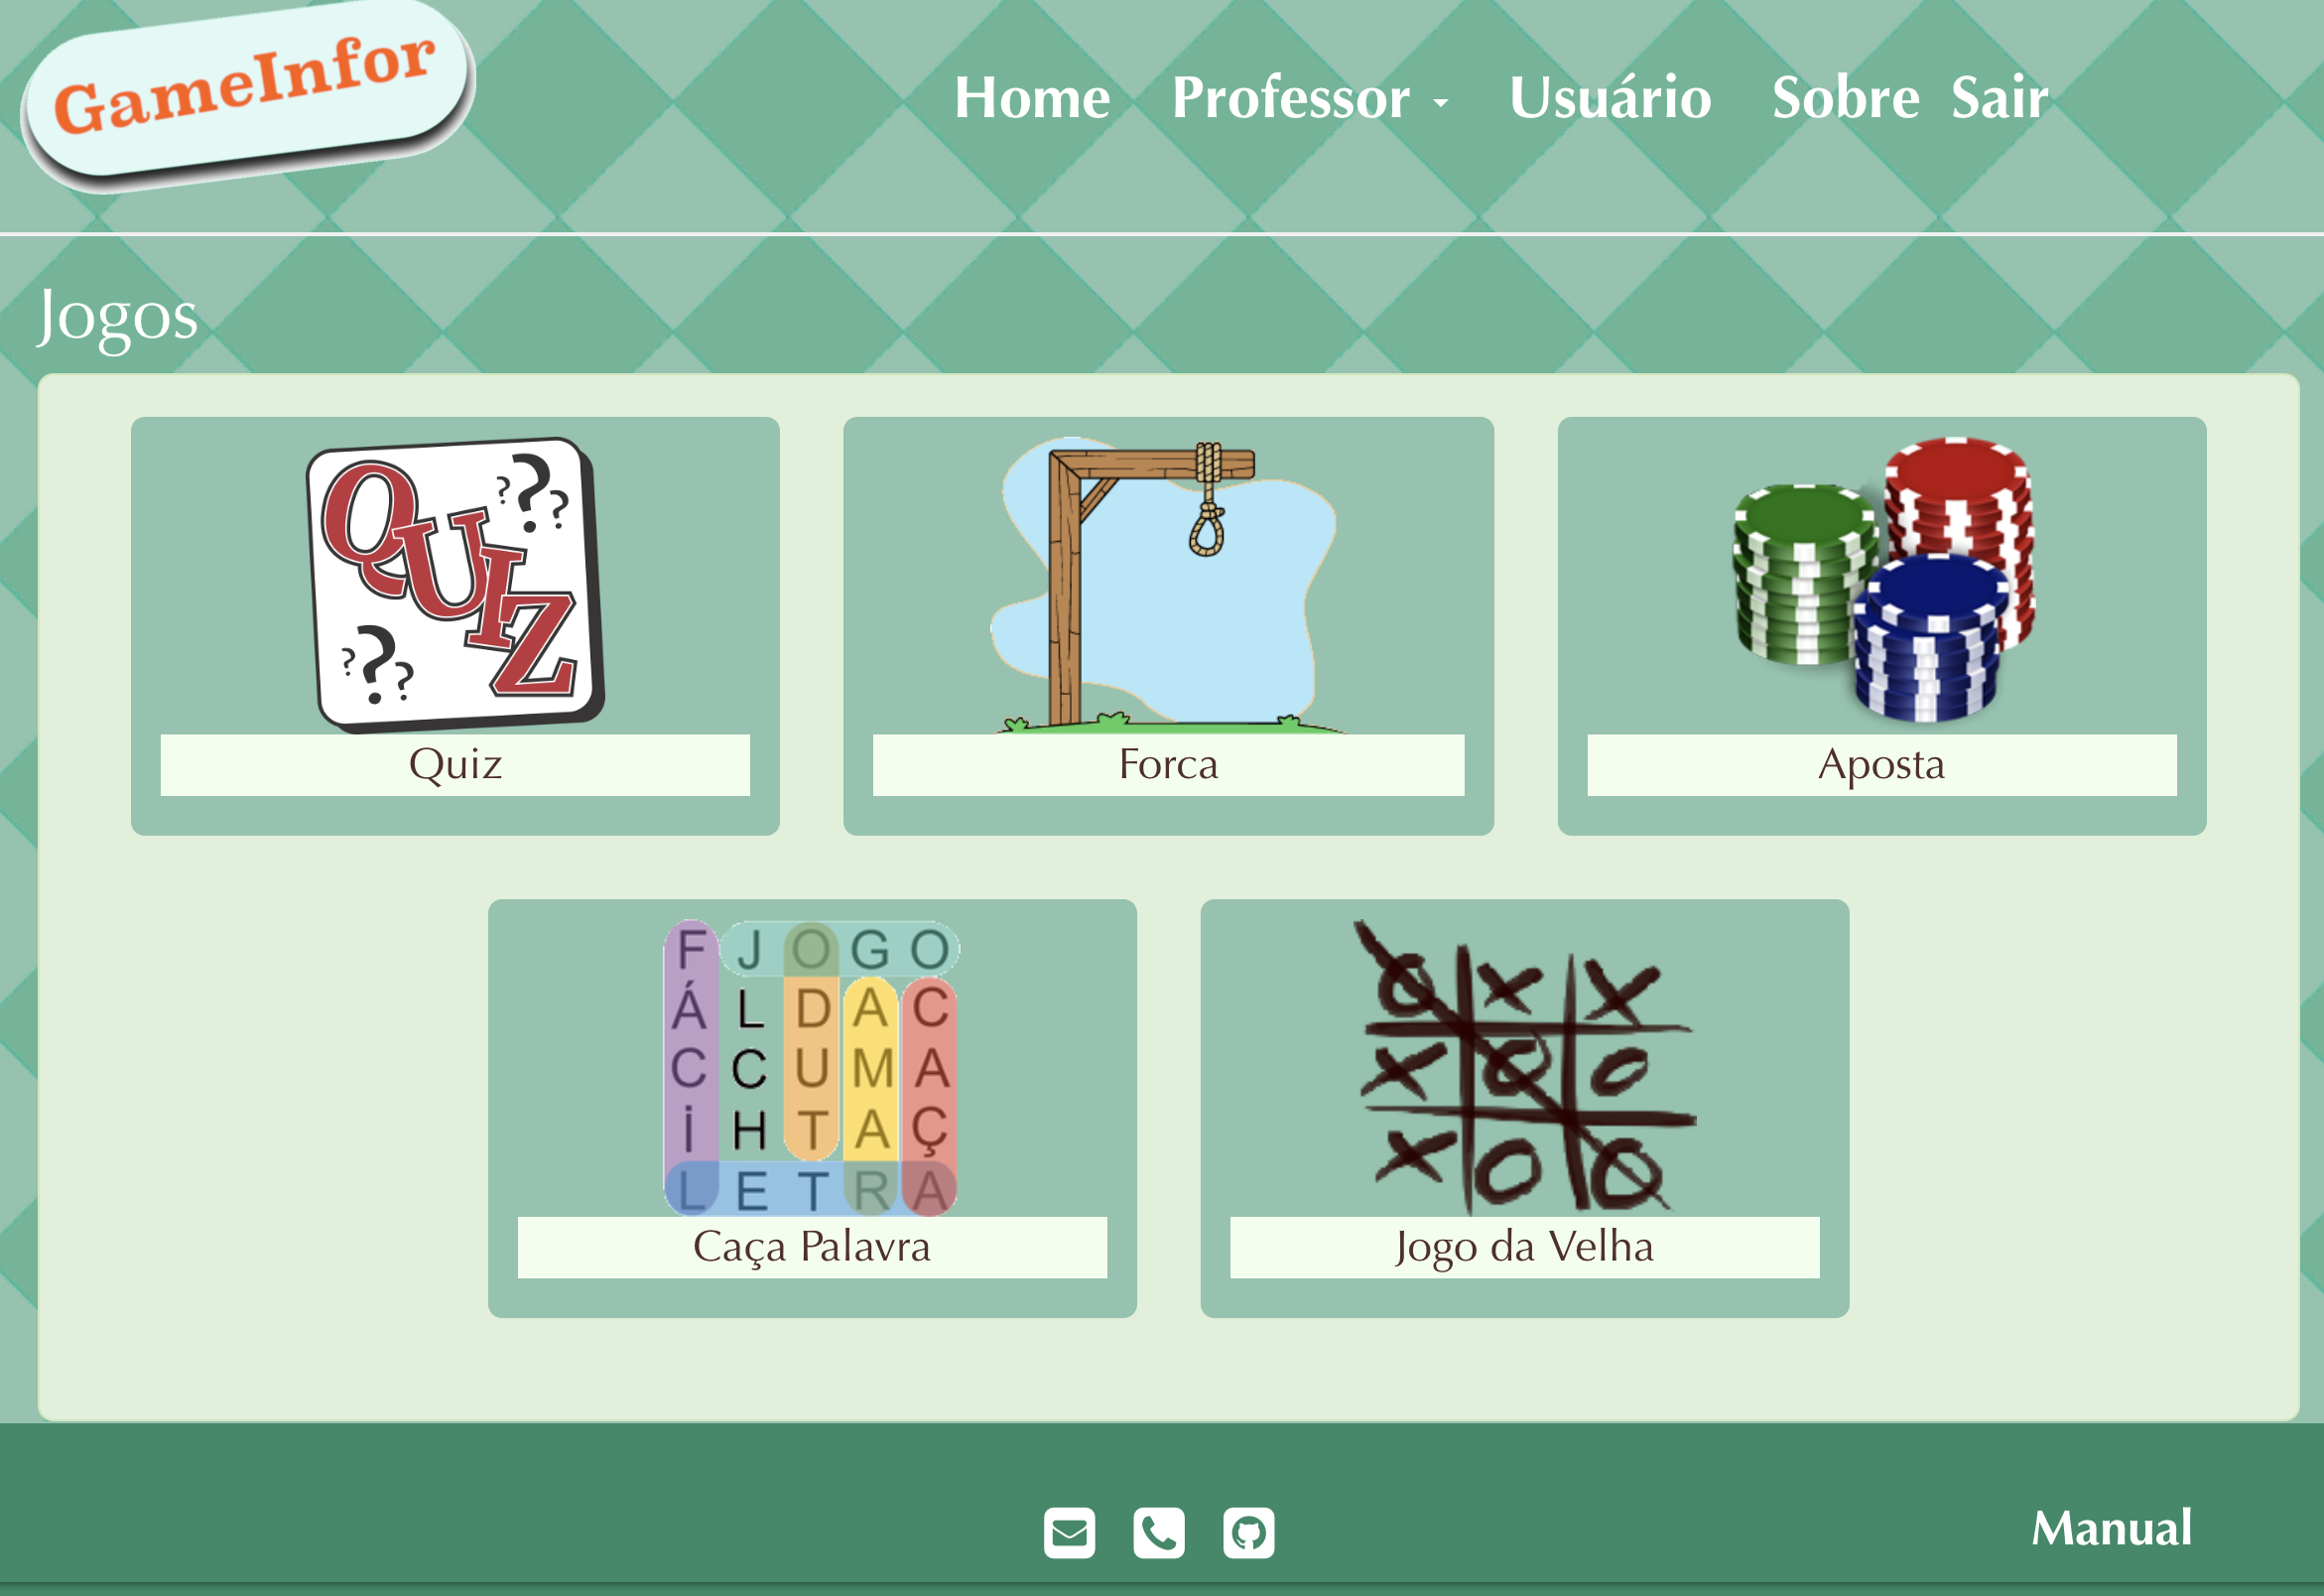
\includegraphics[scale=0.25]{images/proposta-img/Figura4-21.png}
  \caption{Tela de Simulador de Jogo}
  \label{fig:Figura4-21}
\end{figure}

No jogo de Quiz o aluno receberá uma lista de perguntas e determinada quantidade de ajudas, tais como pular pergunta e receber dica da resposta, para cada pergunta será disponibilizado um tempo para responder. Caso acerte o aluno receberá 100 pontos. Ao decorrer do jogo, ele pode usar as ajudas recebidas com o custo de 50 pontos por ajuda.

\begin{figure}[H]
  \centering
  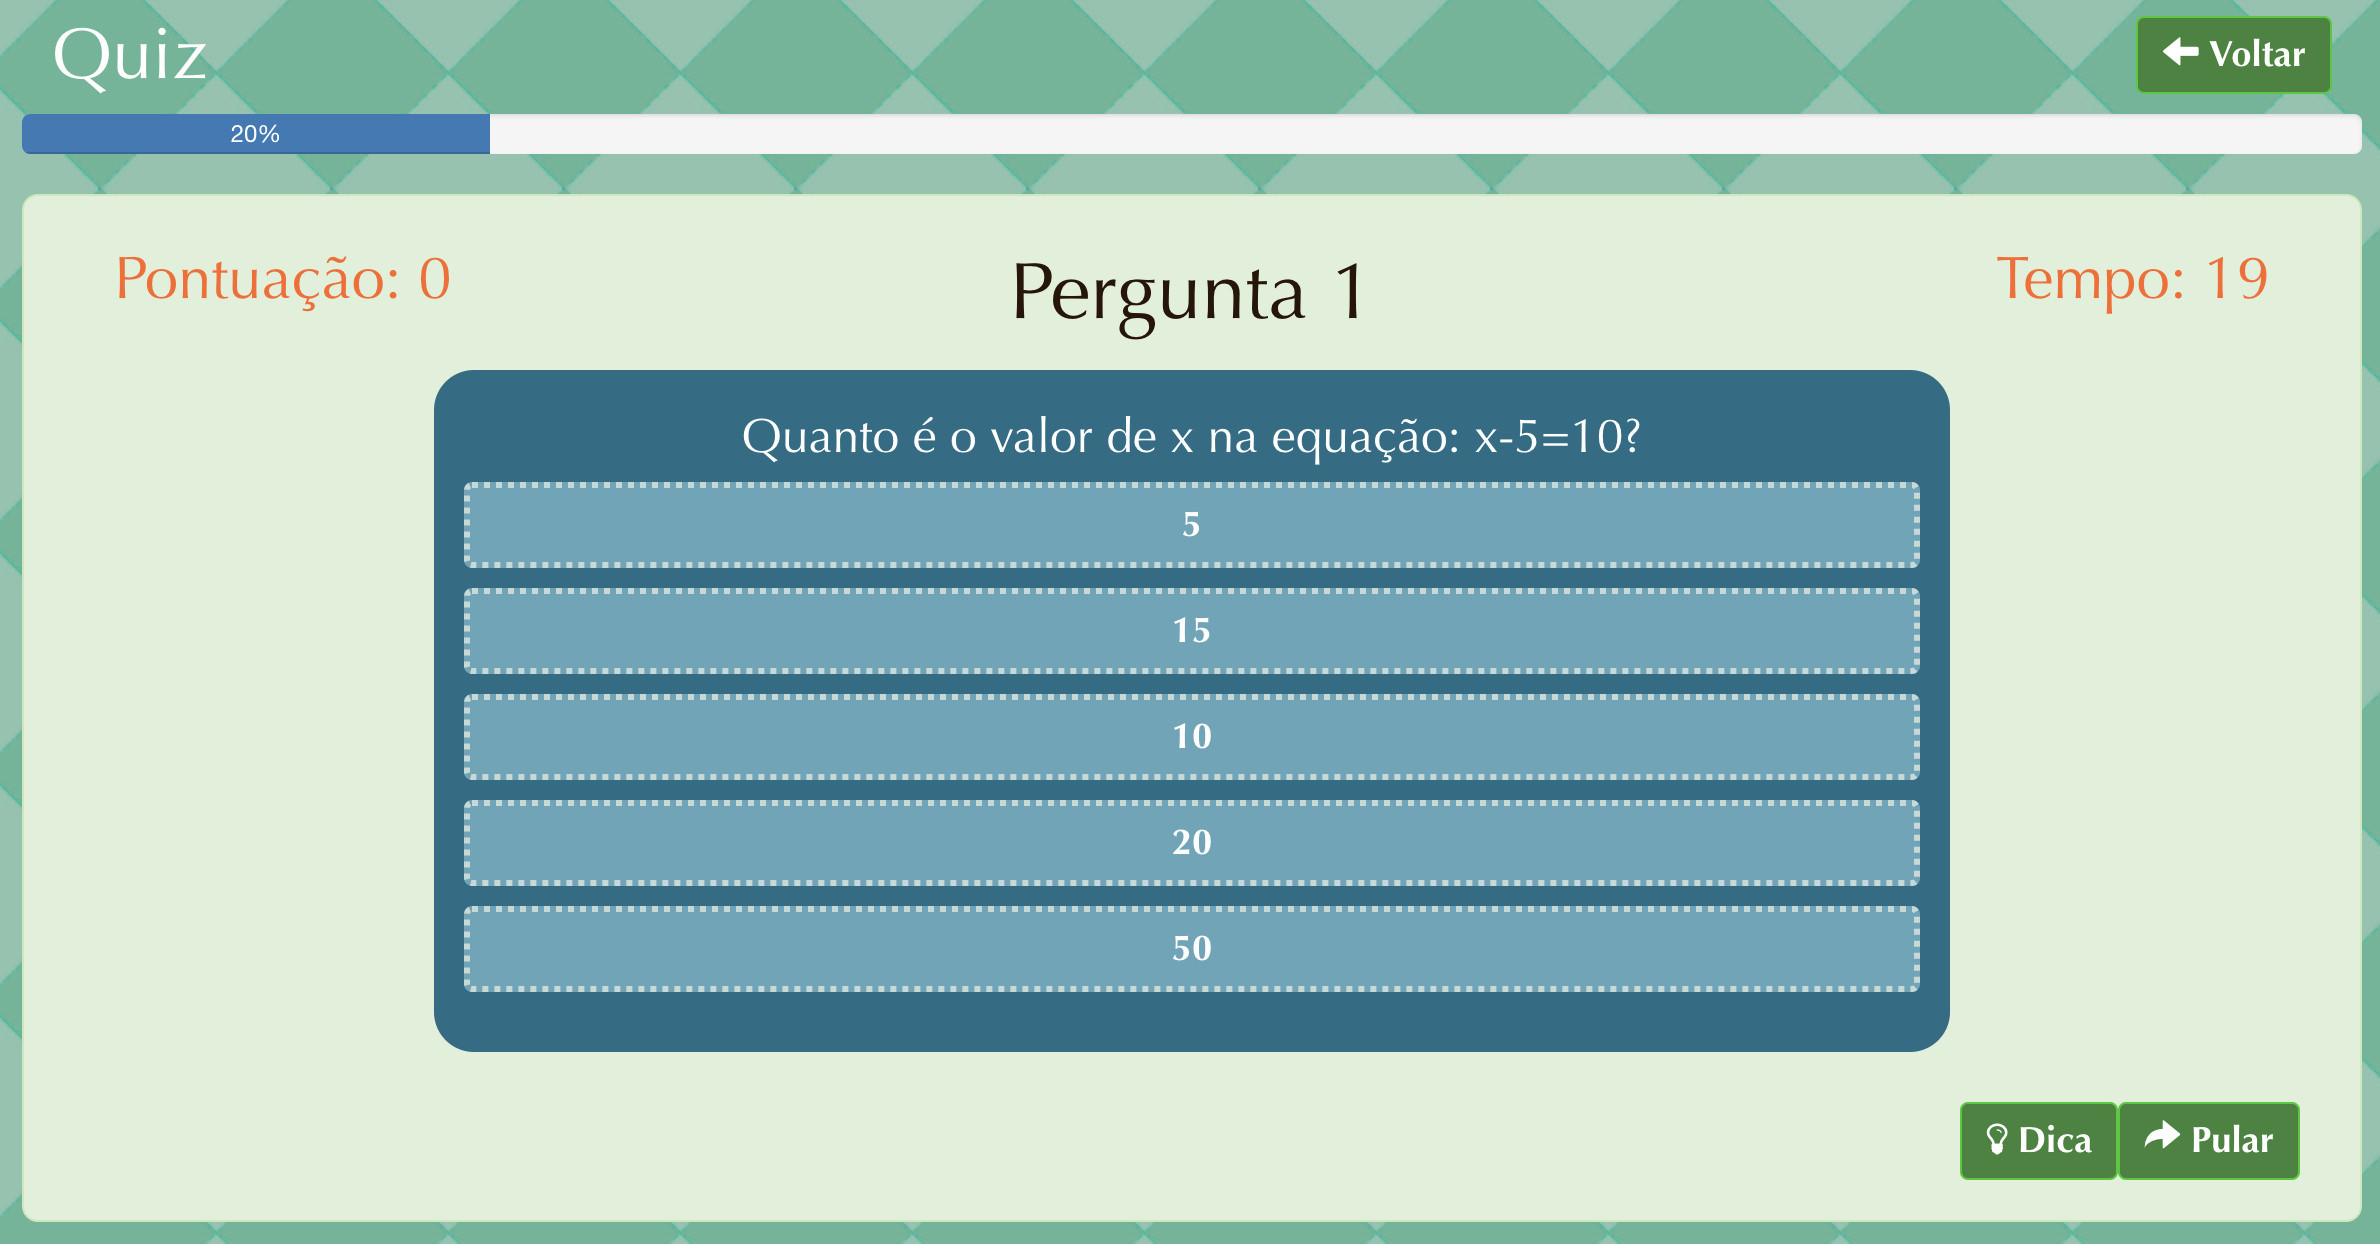
\includegraphics[scale=0.25]{images/proposta-img/Figura4-22.png}
  \caption{Tela do Jogo Quiz}
  \label{fig:Figura4-22}
\end{figure}

Um outro jogo disponível é a Forca, esse jogo funciona da seguinte forma: para cada pergunta será mostrado a quantidade de letras da resposta e o aluno poderá ir chutando letras que estão presentes na resposta. Se o aluno escolher uma grande quantidade de letras erradas ele perde aquela forca e passa para a próxima. Ao final o aluno poderá avançar se tiver acertado uma determinada quantidade de palavras.

\begin{figure}[H]
  \centering
  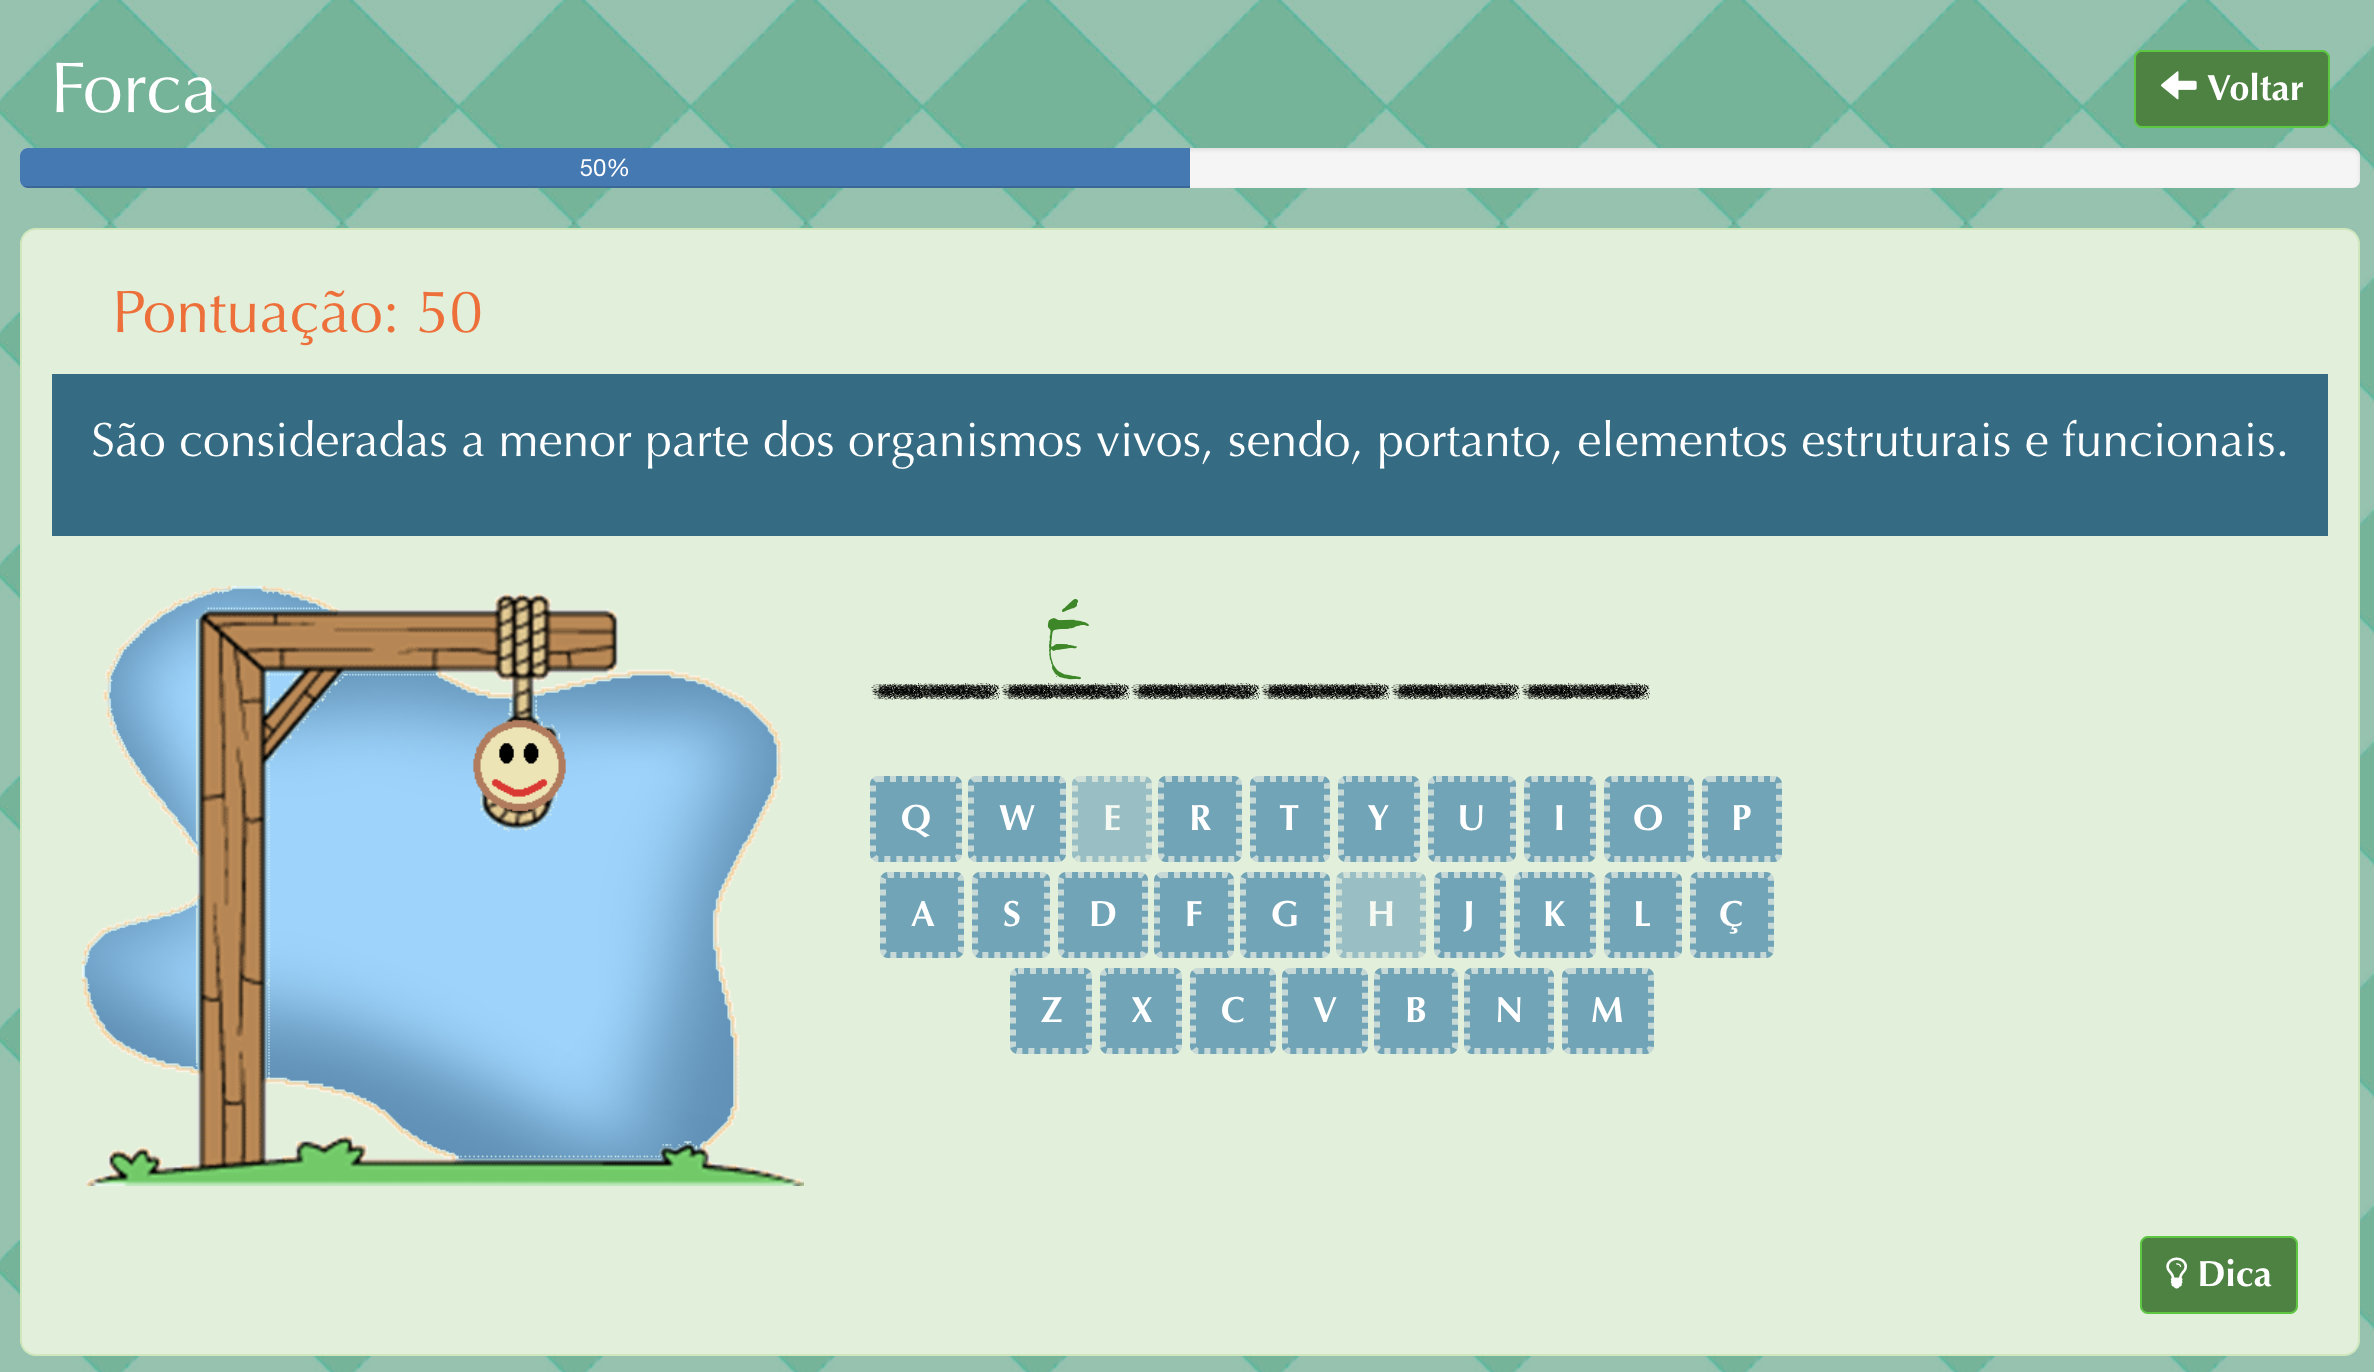
\includegraphics[scale=0.25]{images/proposta-img/Figura4-23.png}
  \caption{Tela do Jogo Forca}
  \label{fig:Figura4-23}
\end{figure}

O professor pode também escolher o jogo das apostas, este jogo funcionará com as seguintes regras: os participantes receberão uma quantidade de fichas no começo; e em cada rodada será feita uma pergunta, logo em seguida dará oportunidade para que o participante faça uma aposta mínima ou aposte quantas fichas achar necessário na resposta que considere a correta. Registra-se que se o aluno terminar a partida com pelo menos 70% das fichas poderá avançar para a próxima fase.

\begin{figure}[H]
  \centering
  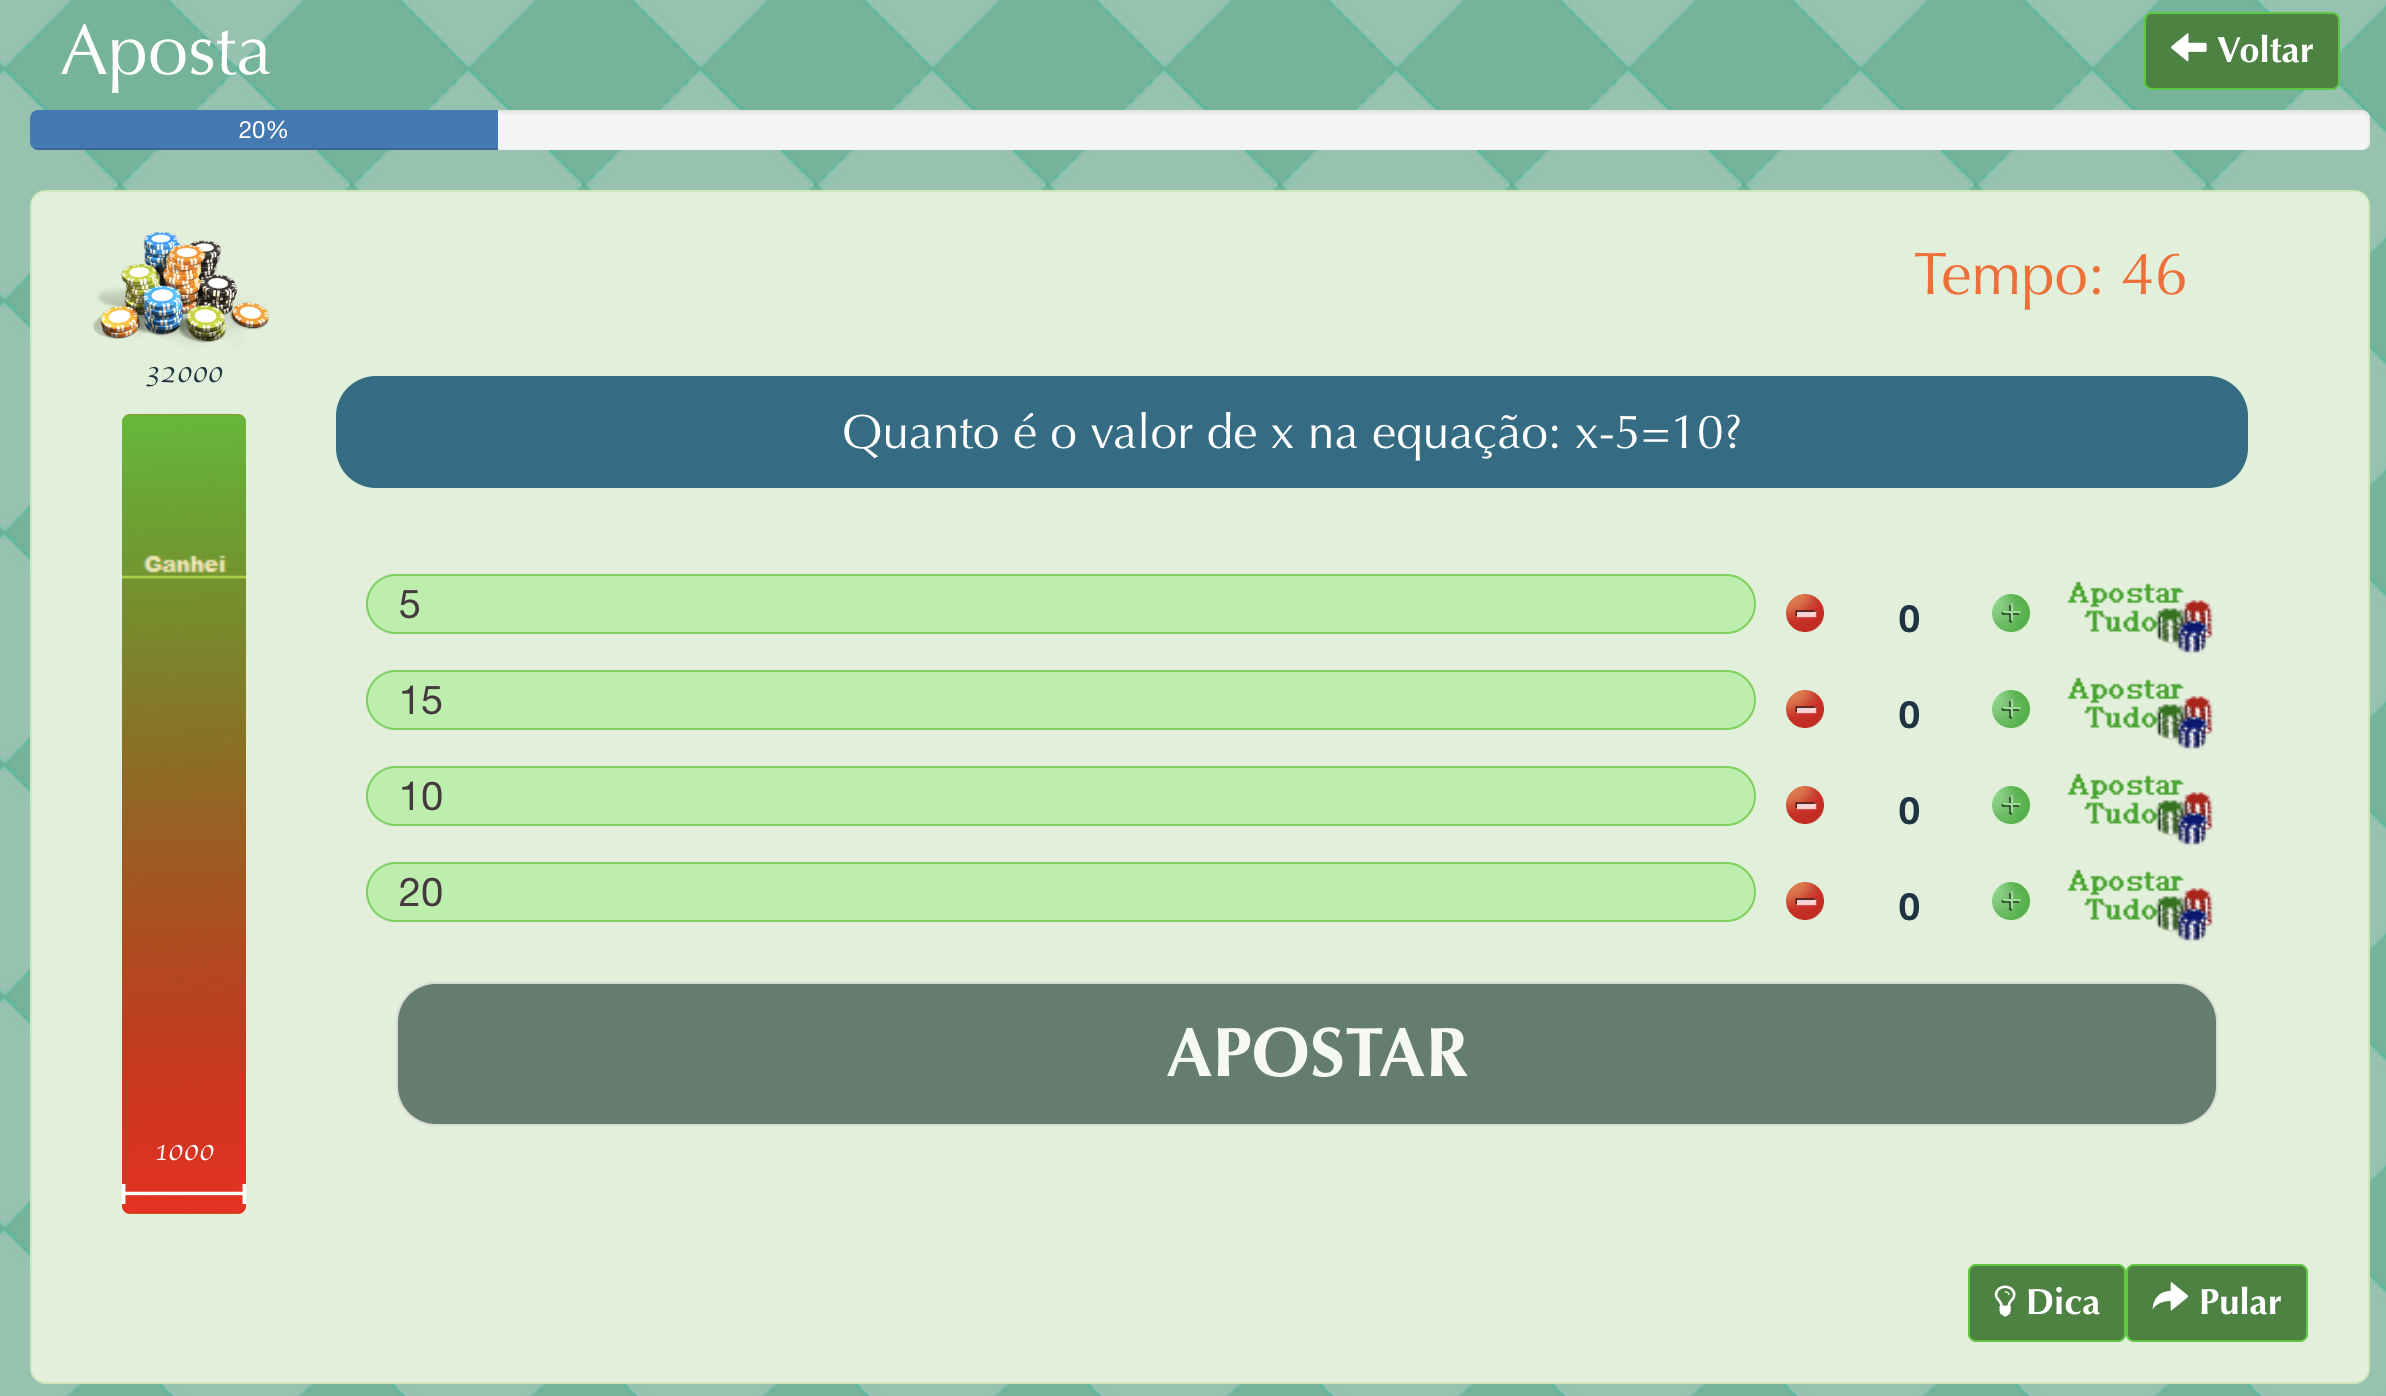
\includegraphics[scale=0.25]{images/proposta-img/Figura4-24.png}
  \caption{Tela do Jogo de Aposta}
  \label{fig:Figura4-24}
\end{figure}

A plataforma ainda disponibiliza o jogo de caça-palavras, neste jogo o usuário receberá uma lista de perguntas e as respostas dessas perguntas encontram-se dentro do jogo de caça-palavra. O aluno deverá marcar as respostas corretas dentro do caça-palavra.

Caso o aluno não encontre as palavras do caça-palavra ele pode passar para o próxima caça palavra ou pedir uma dica. Ao finalizar será feito a soma de pontos das palavras achadas. se foi atingindo uma determinada quantidade de pontos o aluno poderá passar para próxima fase.

\begin{figure}[H]
  \centering
  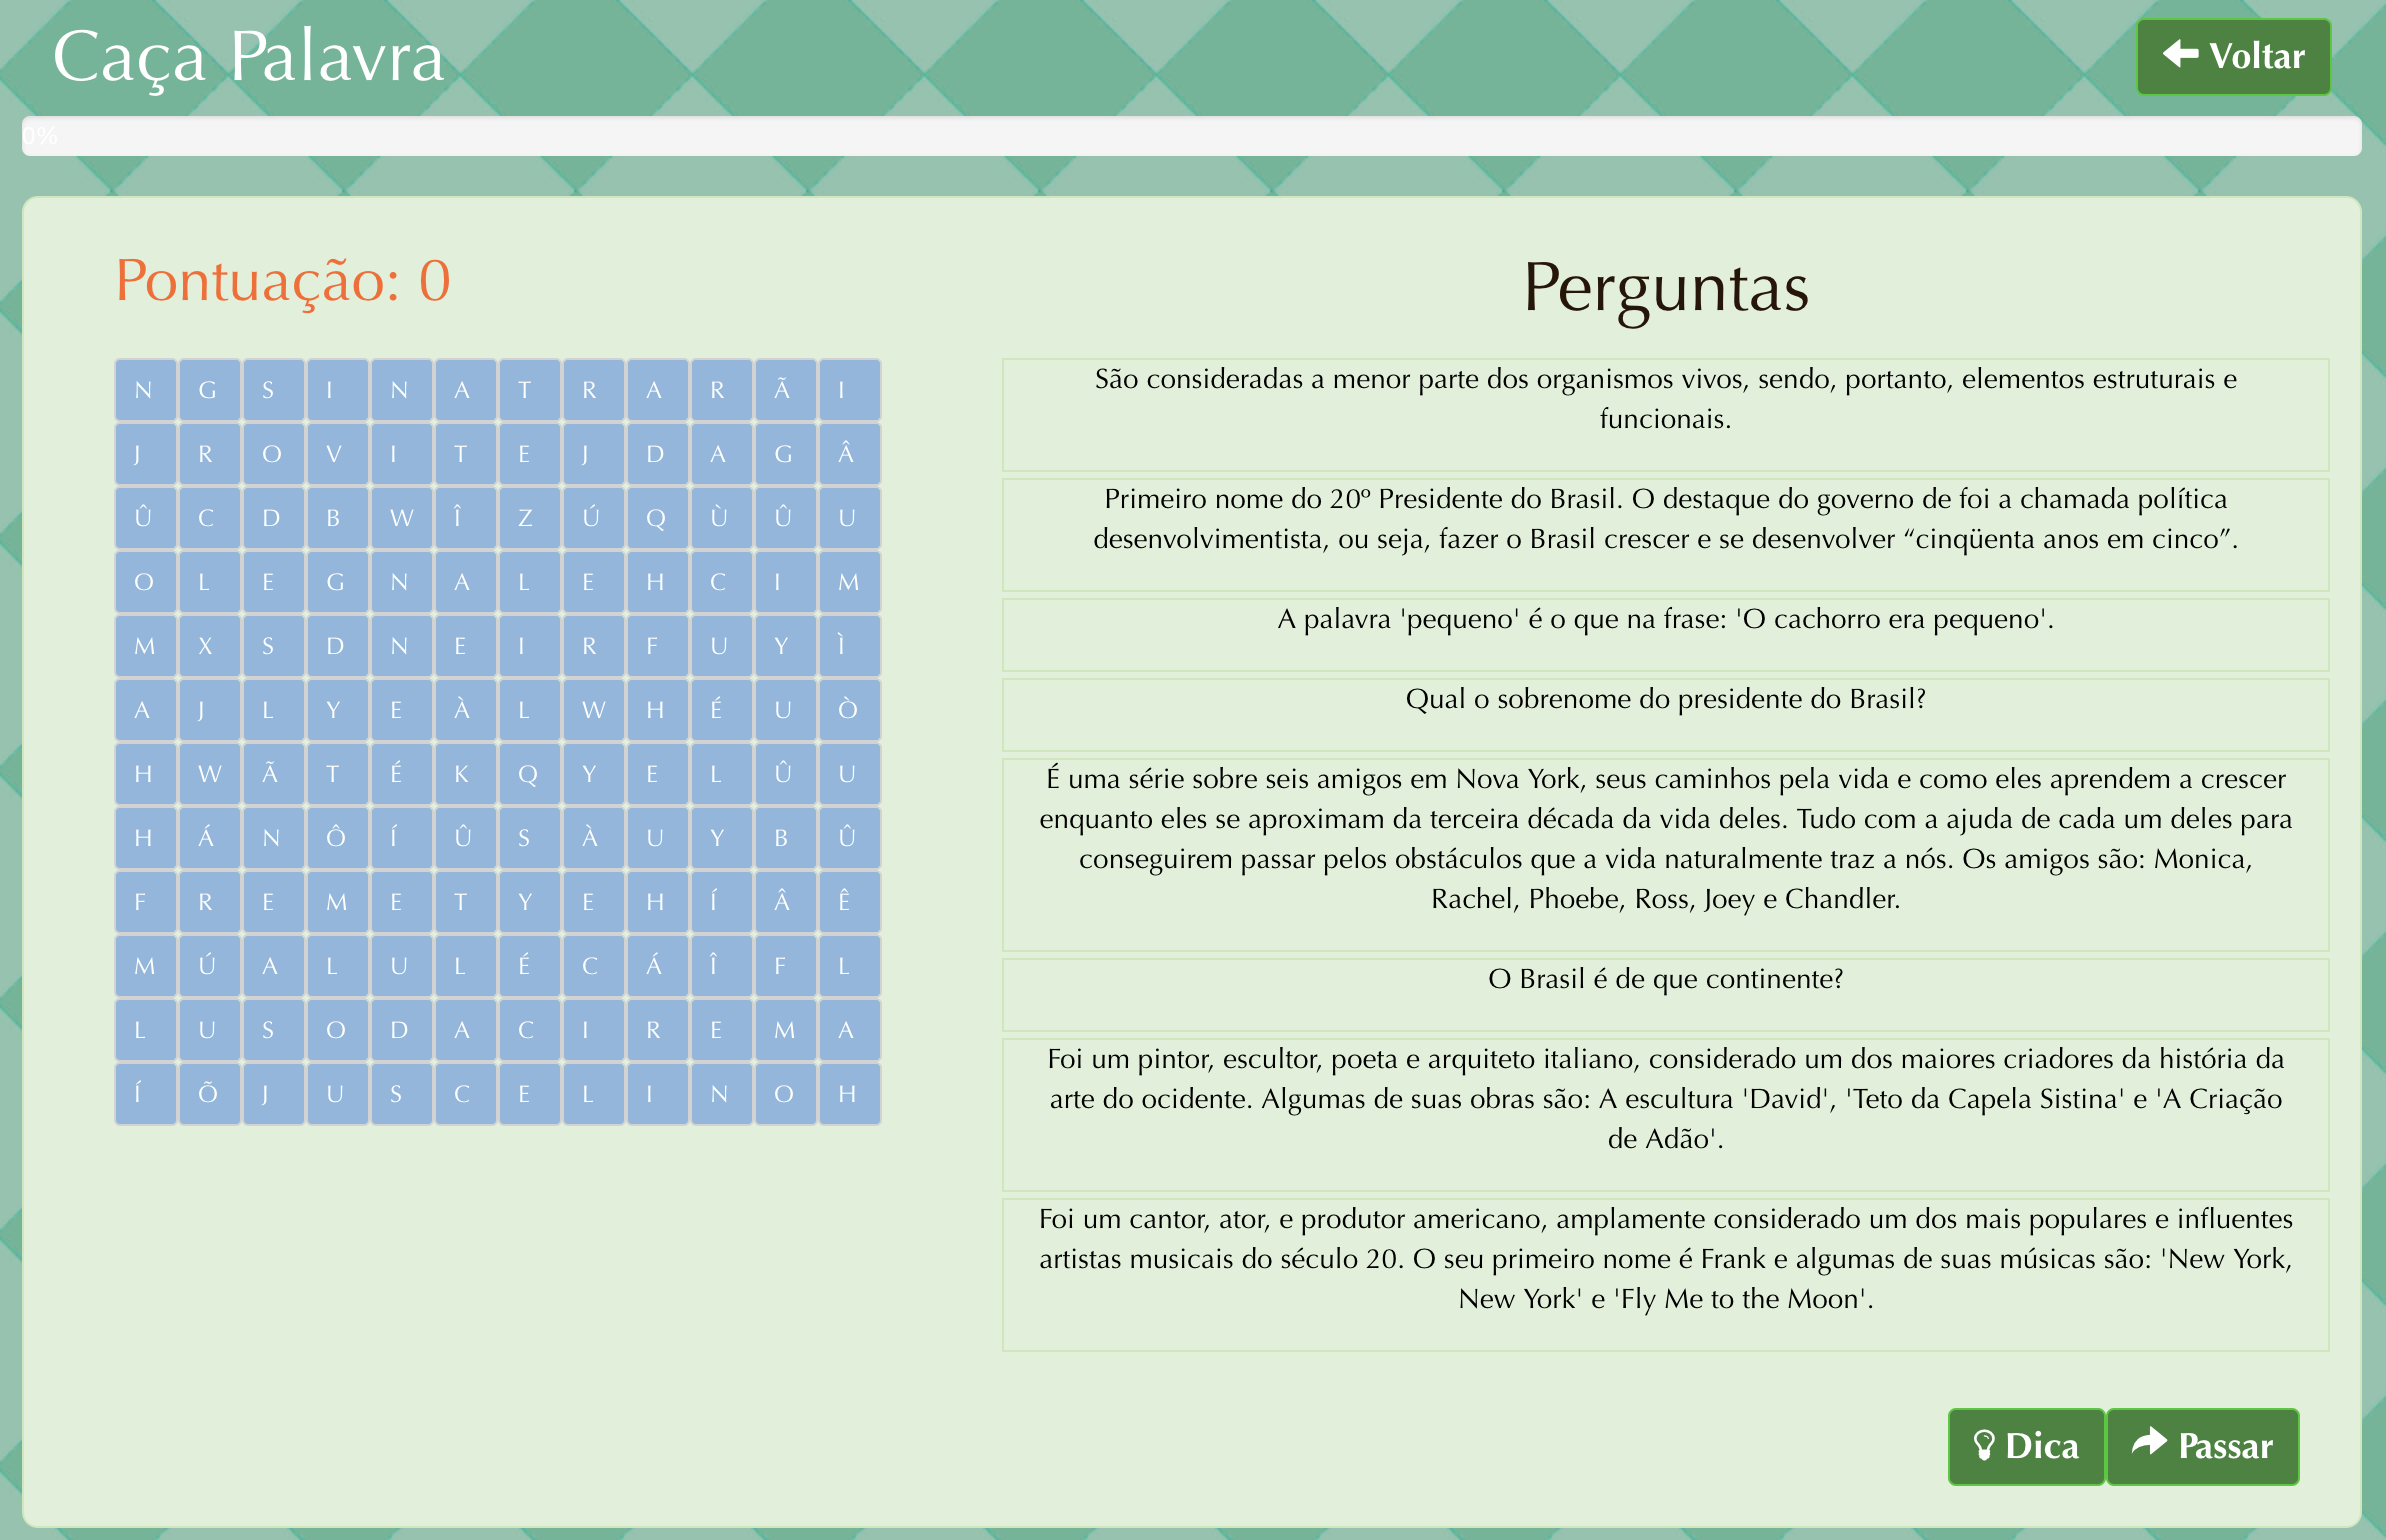
\includegraphics[scale=0.25]{images/proposta-img/Figura4-25.png}
  \caption{Tela do Jogo Caça-Palavra}
  \label{fig:Figura4-25}
\end{figure}

Por fim, o último jogo é o Jogo da Velha, neste jogo o aluno deve jogar contra se mesmo, inicialmente ele escolherá um lugar para fazer a jogada, após realizar essa escolha, aparecerá uma pergunta que ele deve responder, se o aluno responder corretamente, o lugar escolhido será preenchido com um “O”, caso contrário com um “X”. A aluno ganha o jogo quando completar uma linha, coluna ou diagonal com o símbolo “O”.

\begin{figure}[H]
  \centering
  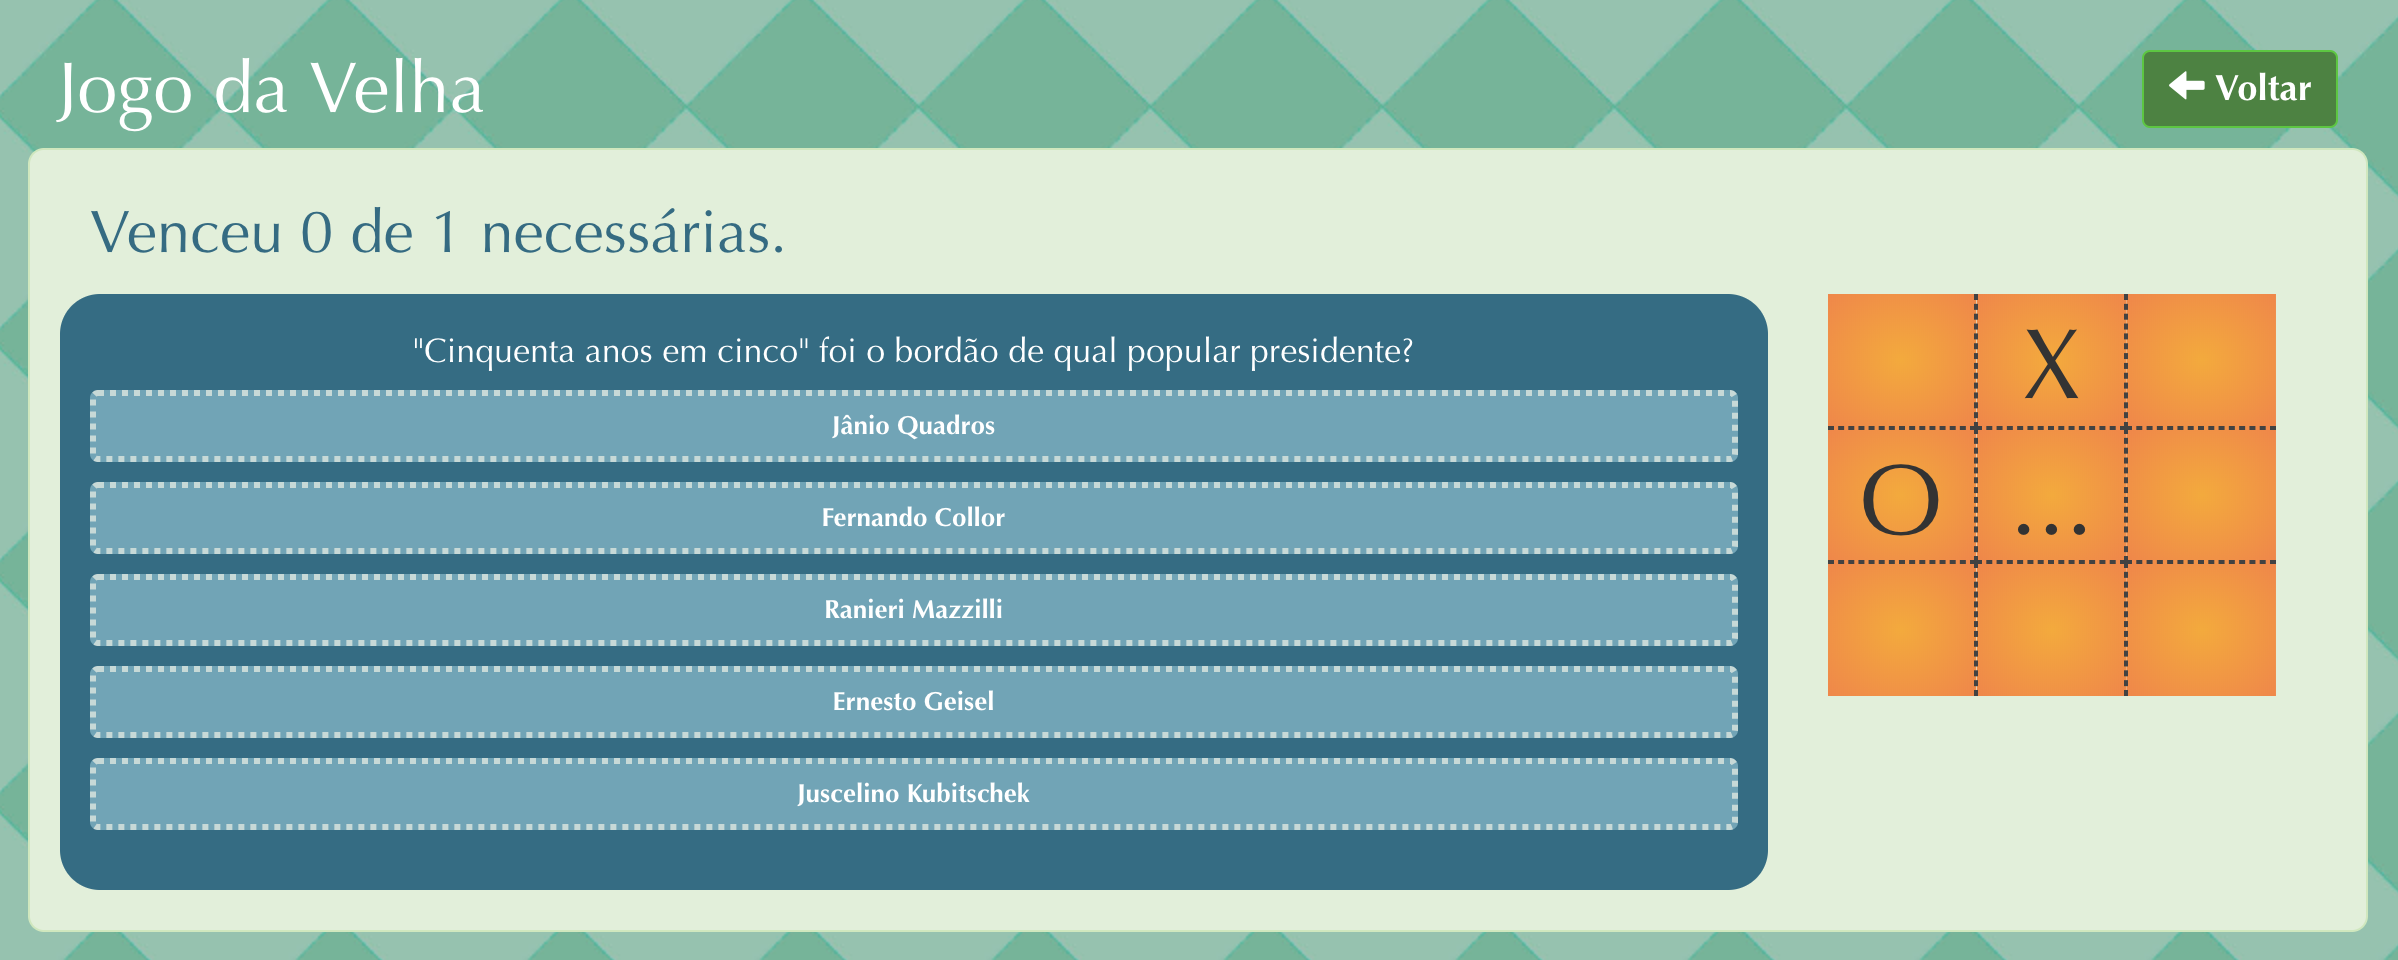
\includegraphics[scale=0.25]{images/proposta-img/Figura4-26.png}
  \caption{Tela da Velha}
  \label{fig:Figura4-26}
\end{figure}

\subsubsection{Simulador de Tabuleiro}

A tela abaixo foi disponibilizada para o professor apenas com o intuito de ele visualizar como o aluno verá os cursos, cada caixa com o cadeado representa um fase do curso, a medida que que o aluno for avançando nas fases os cadeado serão abertos.

\begin{figure}[H]
  \centering
  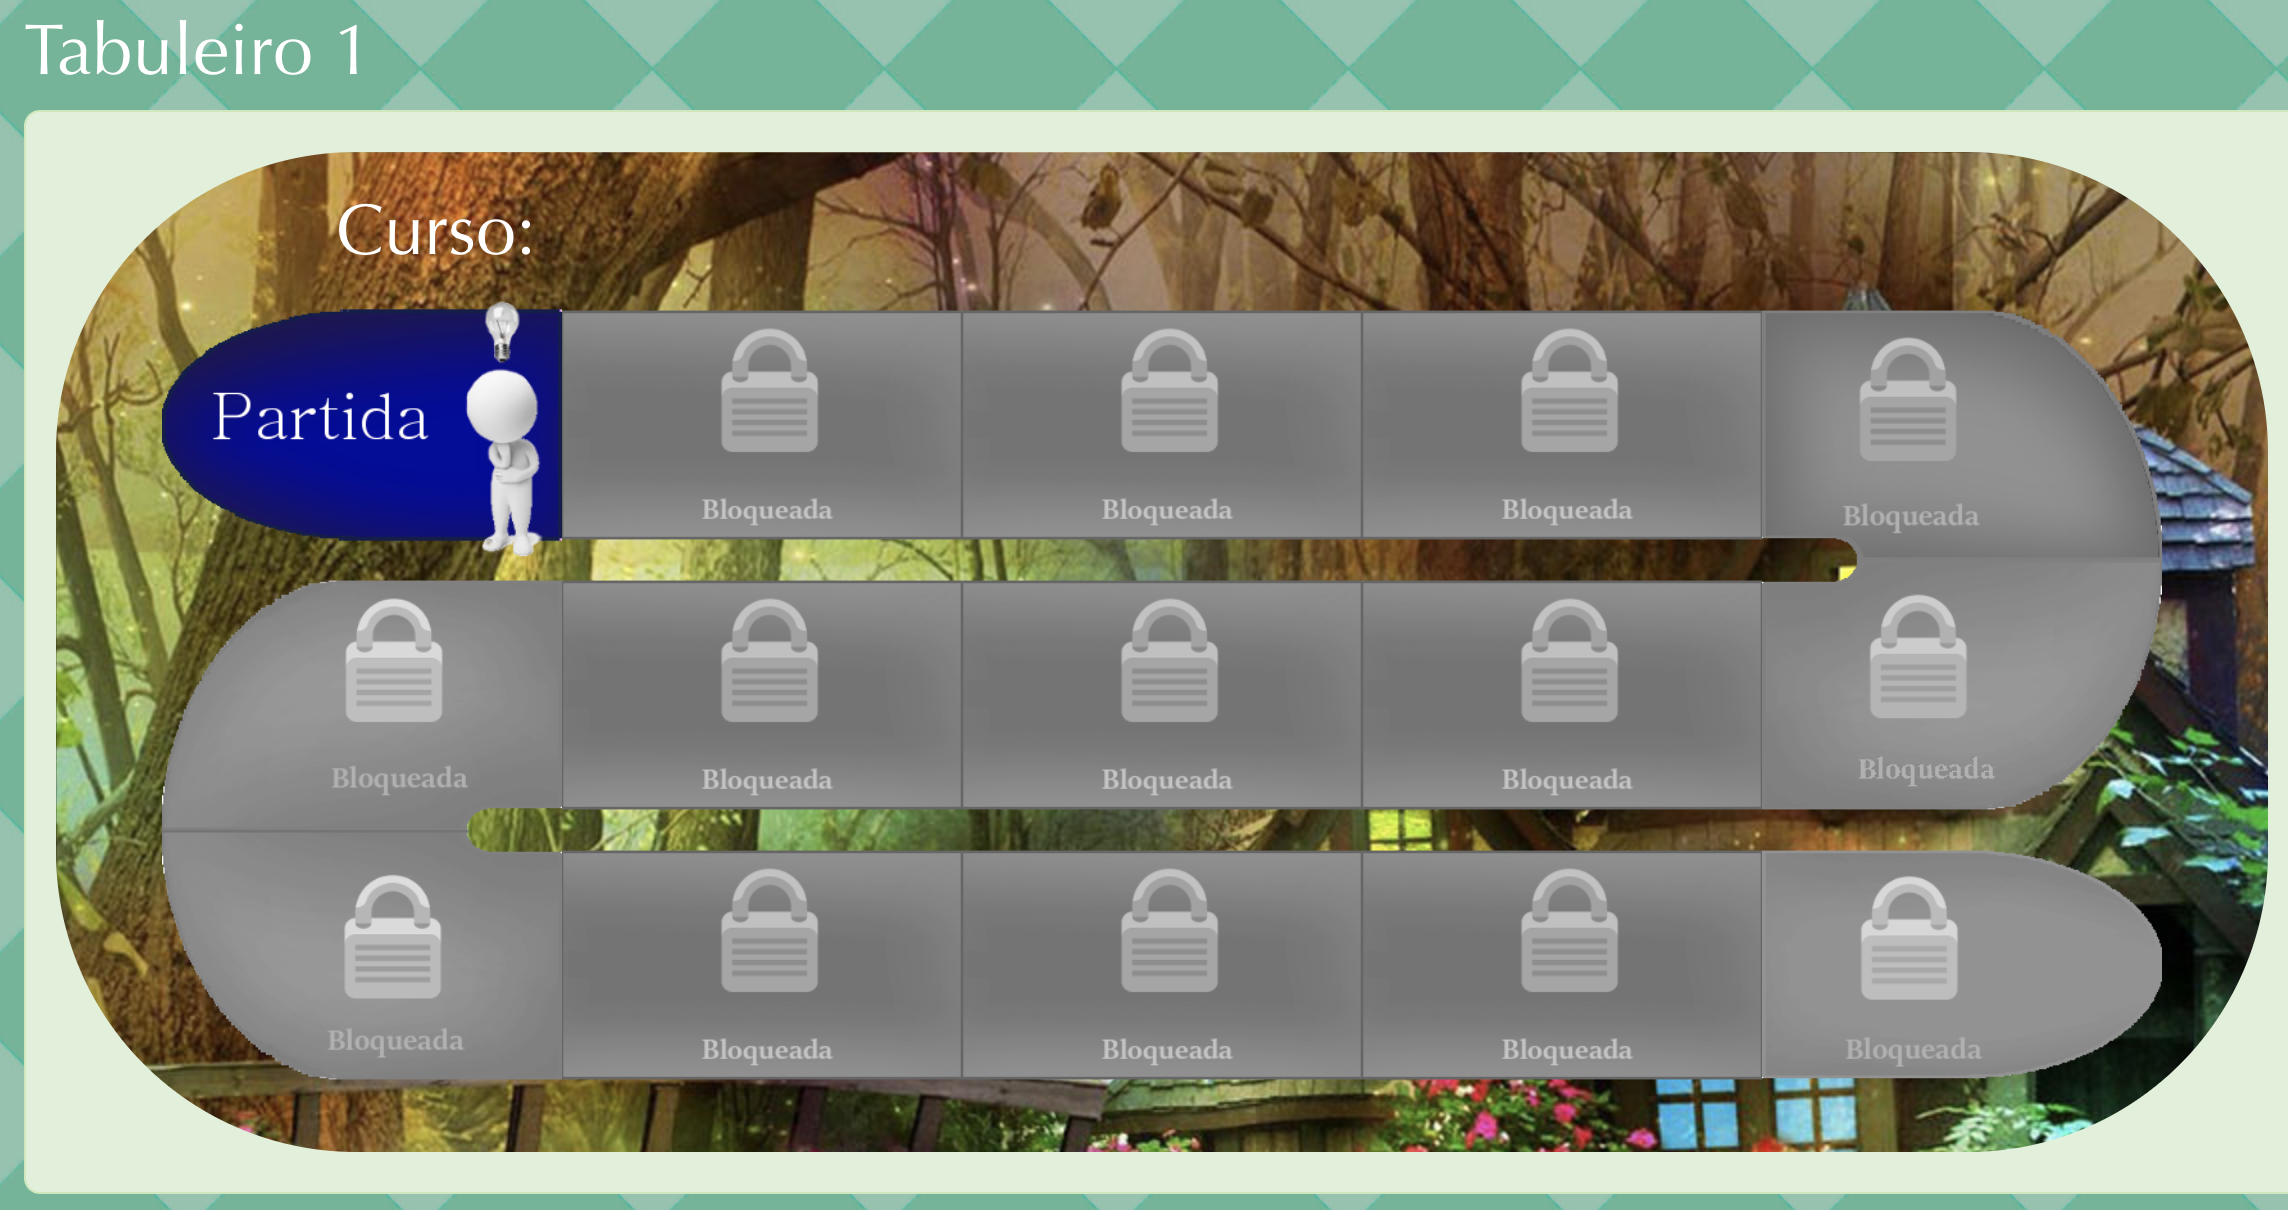
\includegraphics[scale=0.3]{images/proposta-img/Figura4-27.png}
  \caption{Tela de Simulador de Tabuleiro}
  \label{fig:Figura4-27}
\end{figure}

\subsubsection{Dados dos Curso}

A principal ação que um professor pode realizar na plataforma é criar cursos, para fazer isso ele deve acessar o menu do Professor e selecionar “Consultar Curso” e clicar no botão “Novo Curso” mostrado em \figref{fig:Figura4-28}, a seguir é necessário que o professor preencha os campos obrigatórios, e clique em Próximo para começar a criar etapas na tela \figref{fig:Figura4-30}. Vale destacar que o professor tem a opção de adicionar um anexo na criação do curso.

\begin{figure}[H]
  \centering
  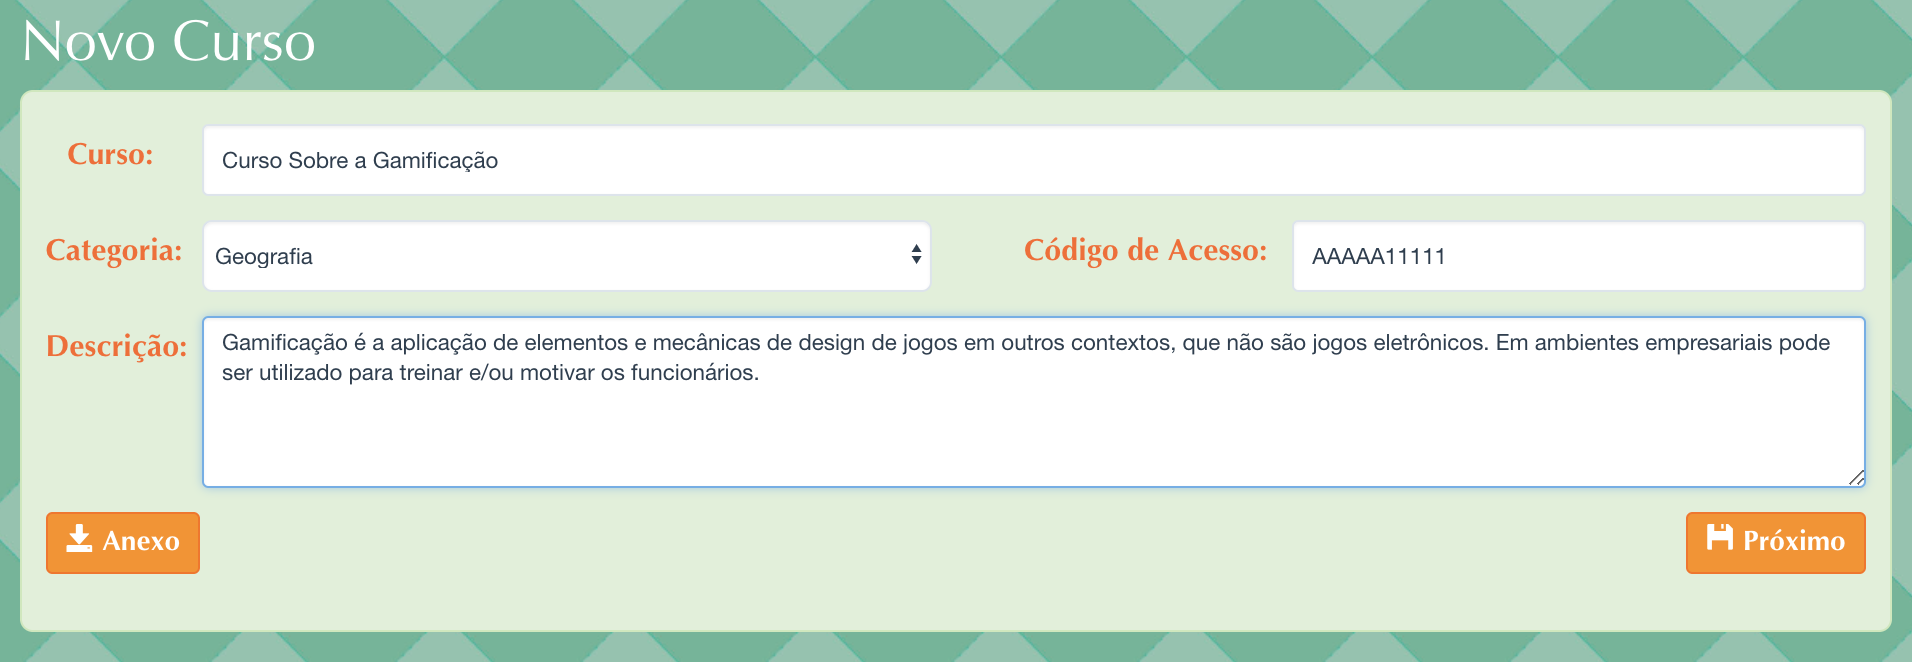
\includegraphics[scale=0.4]{images/proposta-img/Figura4-28.png}
  \caption{Tela de Cadastrar Curso}
  \label{fig:Figura4-28}
\end{figure}

\begin{figure}[H]
  \centering
  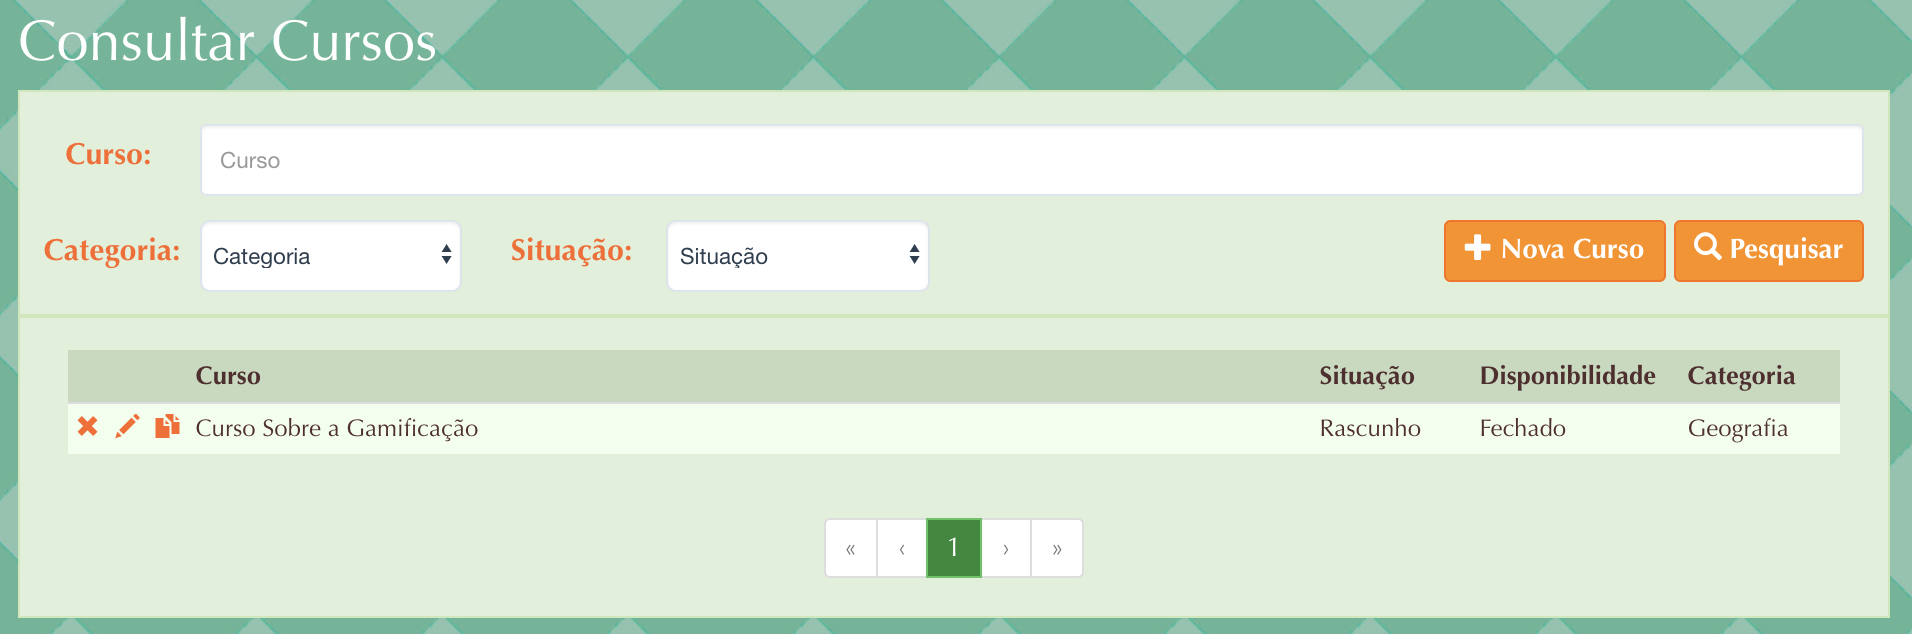
\includegraphics[scale=0.45]{images/proposta-img/Figura4-29.png}
  \caption{Tela de Consultar Curso}
  \label{fig:Figura4-29}
\end{figure}

Na criação das etapas do curso (\figref{fig:Figura4-30}), o professor deve inserir um assunto, um jogo e uma série de perguntas que serão associadas ao jogo selecionado. Para adicionar as perguntas ele deve clicar no botão “Adicionar Perguntas”, a seguir o sistema abrirá uma tela em que é possível consultar as perguntas e selecionar todas que desejar (\figref{fig:Figura4-31}).

Após os dados de cada etapa ter sido preenchidos, é dado ao professor a opção de finalizar o curso ou criar uma nova etapa.

\begin{figure}[H]
  \centering
  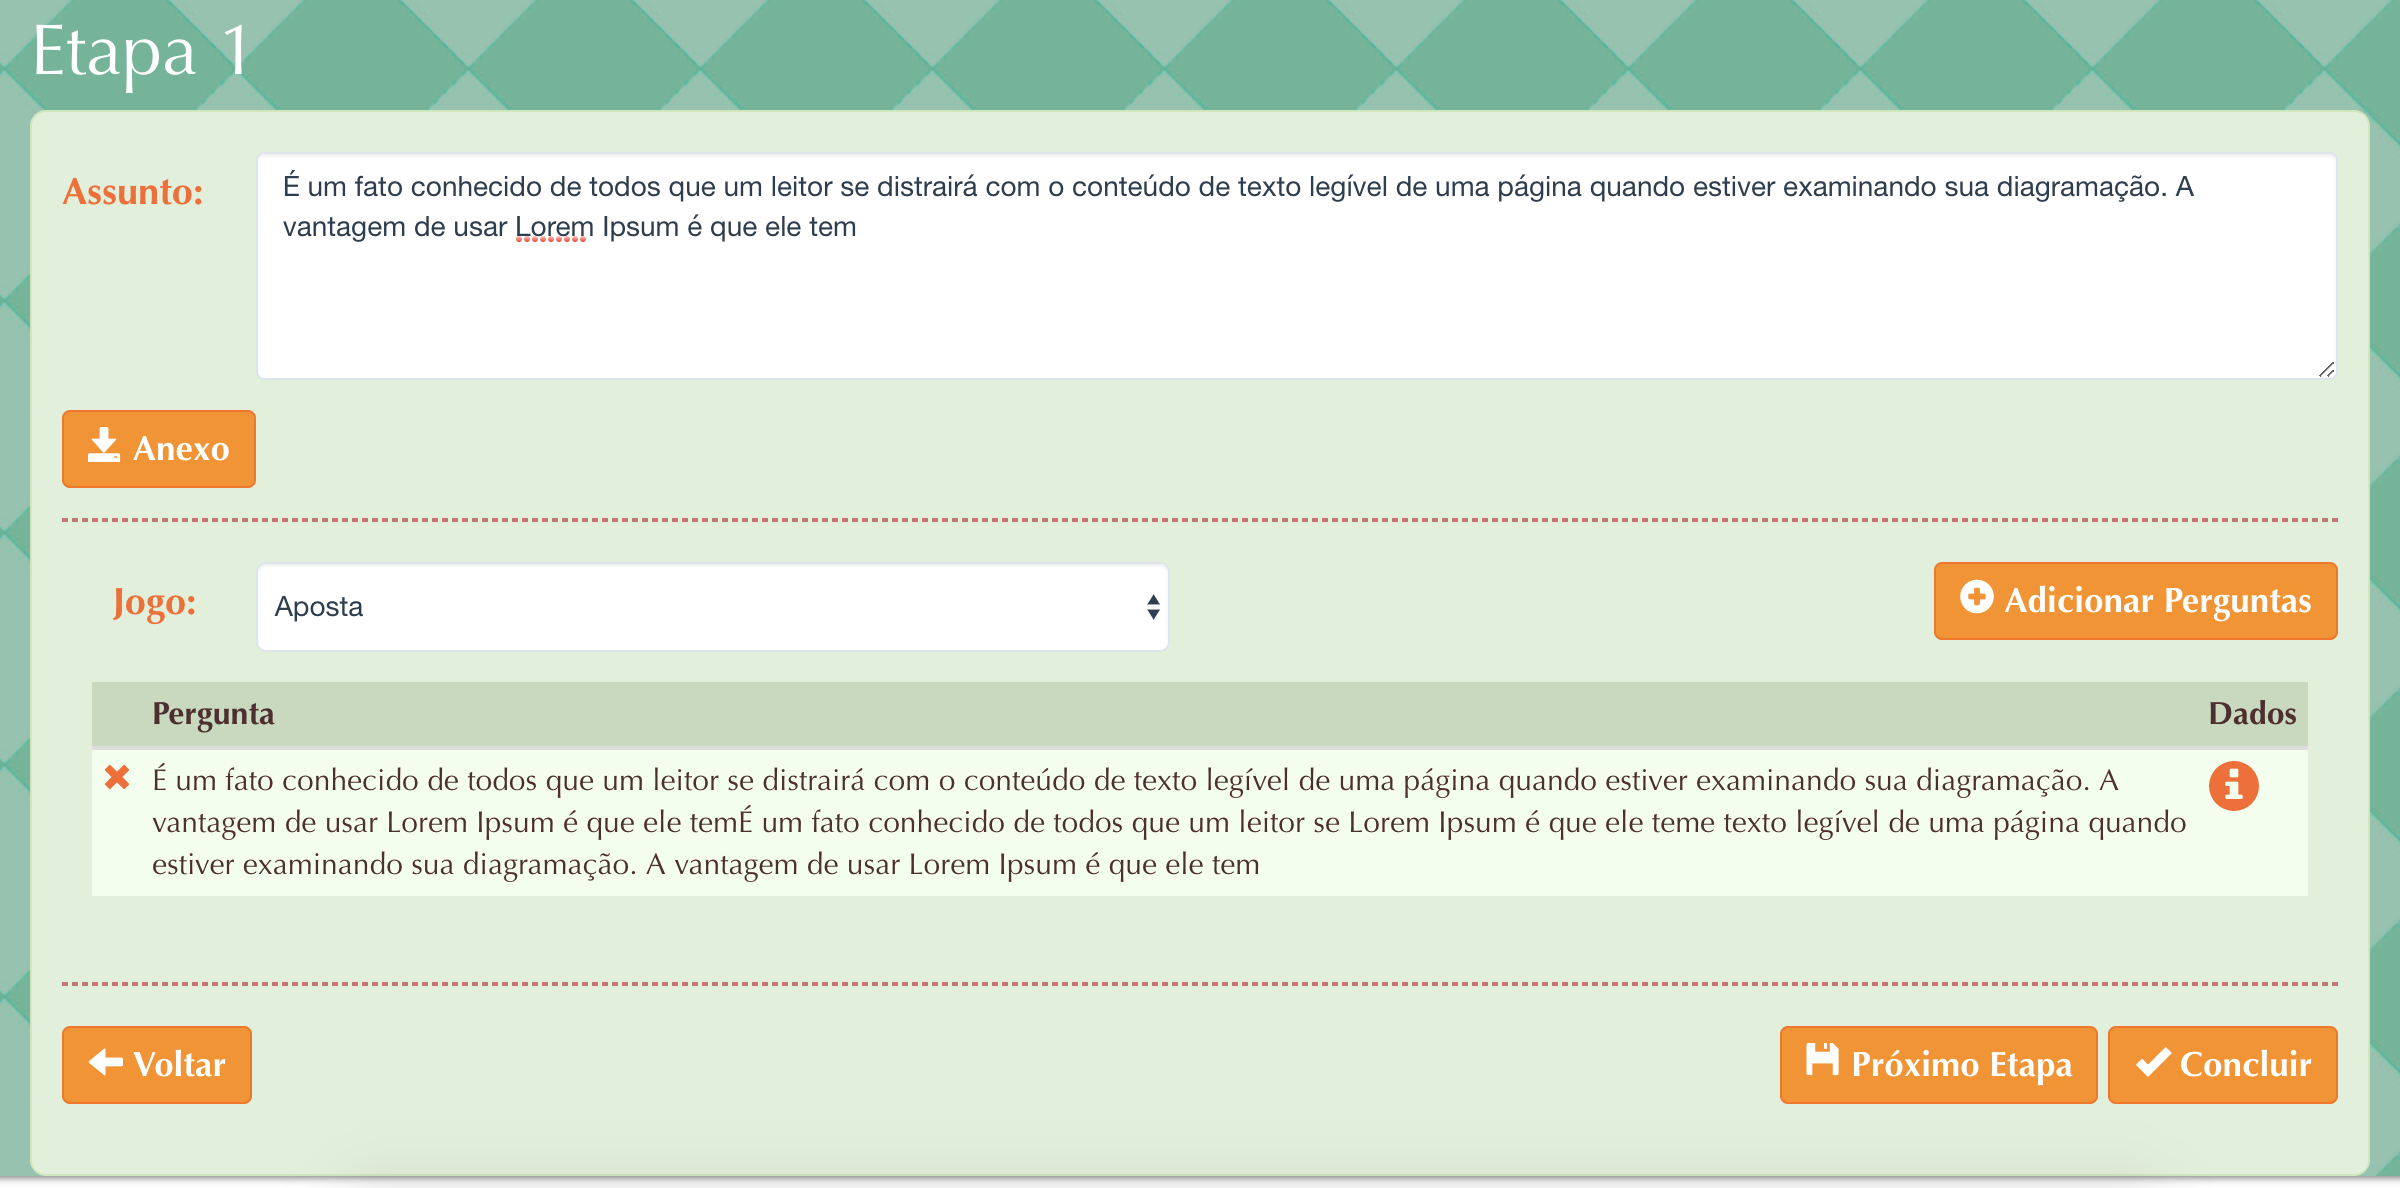
\includegraphics[scale=0.35]{images/proposta-img/Figura4-30.png}
  \caption{Tela de Cadastrar Etapa}
  \label{fig:Figura4-30}
\end{figure}

\begin{figure}[H]
  \centering
  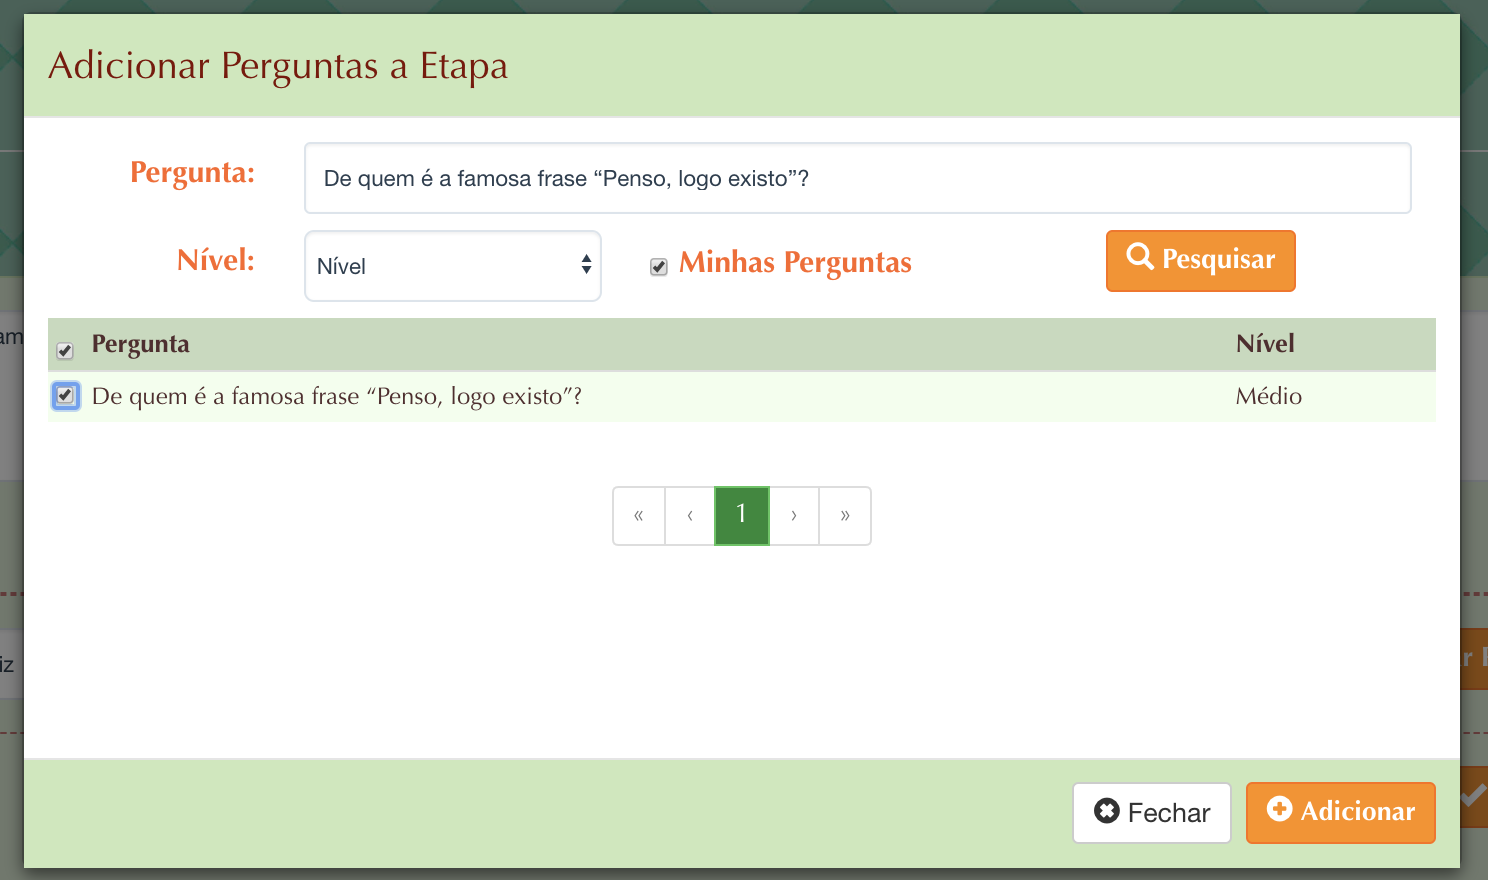
\includegraphics[scale=0.5]{images/proposta-img/Figura4-31.png}
  \caption{Tela de Adicionar Pergunta a Etapa}
  \label{fig:Figura4-31}
\end{figure}

Após a conclusão do curso, o professor pode acompanhar o curso e adicionar  ou visualizar os alunos, além disso, também é possível deixar avisos e recados para os aluno cadastrados no curso.  O curso ficará disponível para os alunos enquanto o professor não encerrar o mesmo, apertando no botão “Encerrar Curso” da \figref{fig:Figura4-32}.

\begin{figure}[H]
  \centering
  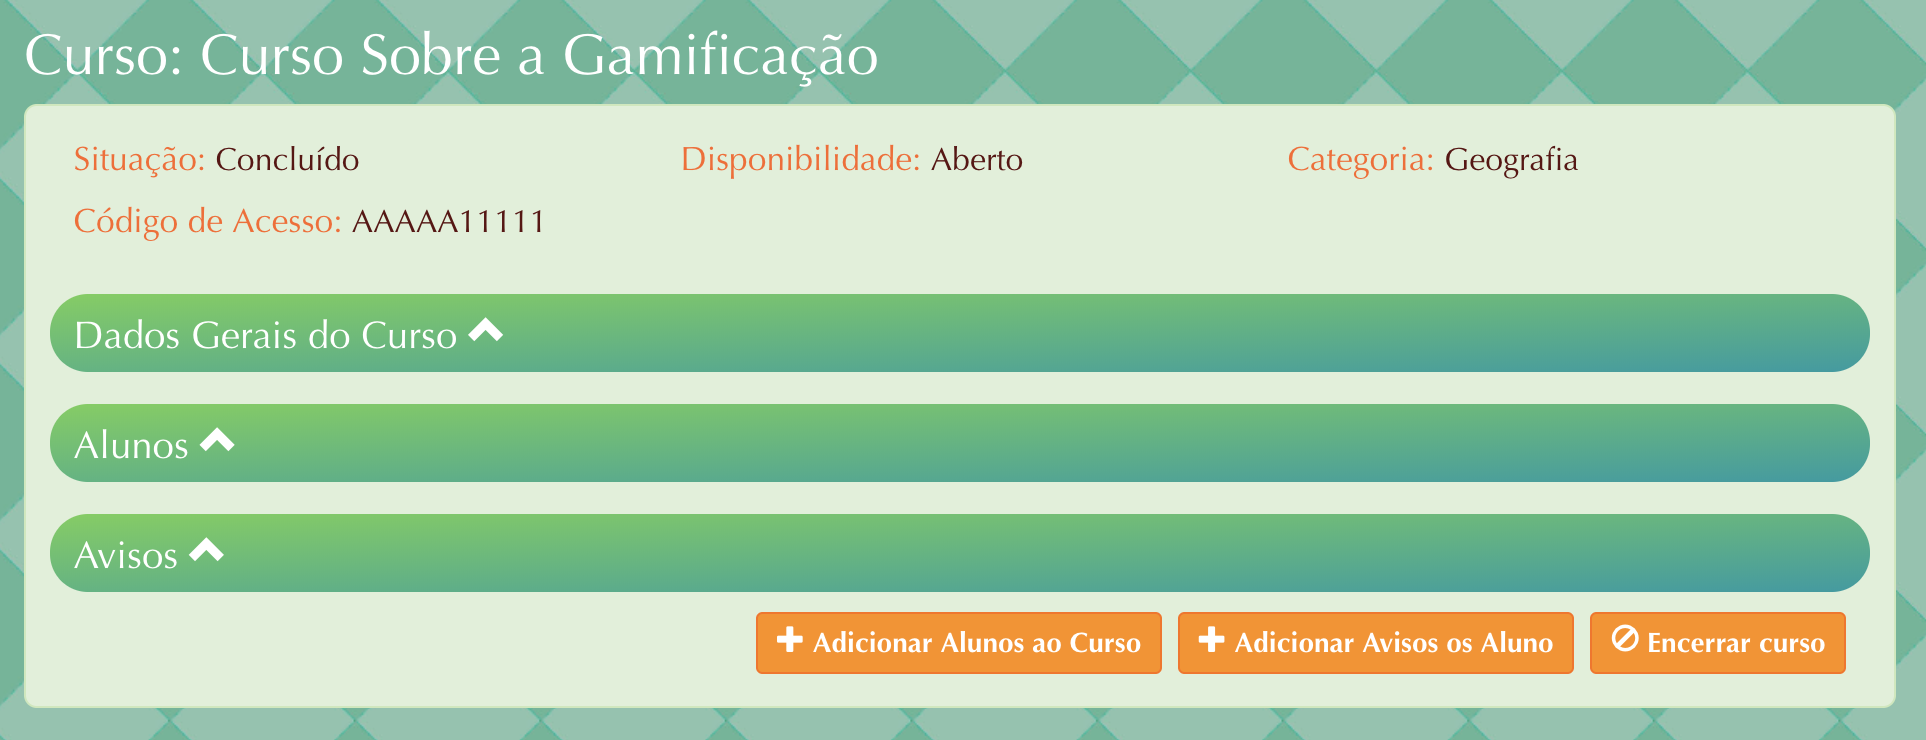
\includegraphics[scale=0.45]{images/proposta-img/Figura4-32.png}
  \caption{Tela de Resumo do Curso}
  \label{fig:Figura4-32}
\end{figure}

Existem duas formas de um aluno entrar em um curso, a primeira é o próprio aluno pesquisar o curso e informar o “Código de Acesso” cadastrado pelo professor, a segunda forma é o professor adicionar alunos por meio do botão “Adicionar Alunos ao Curso” disponibilizado na imagem \figref{fig:Figura4-32}.

\begin{figure}[H]
  \centering
  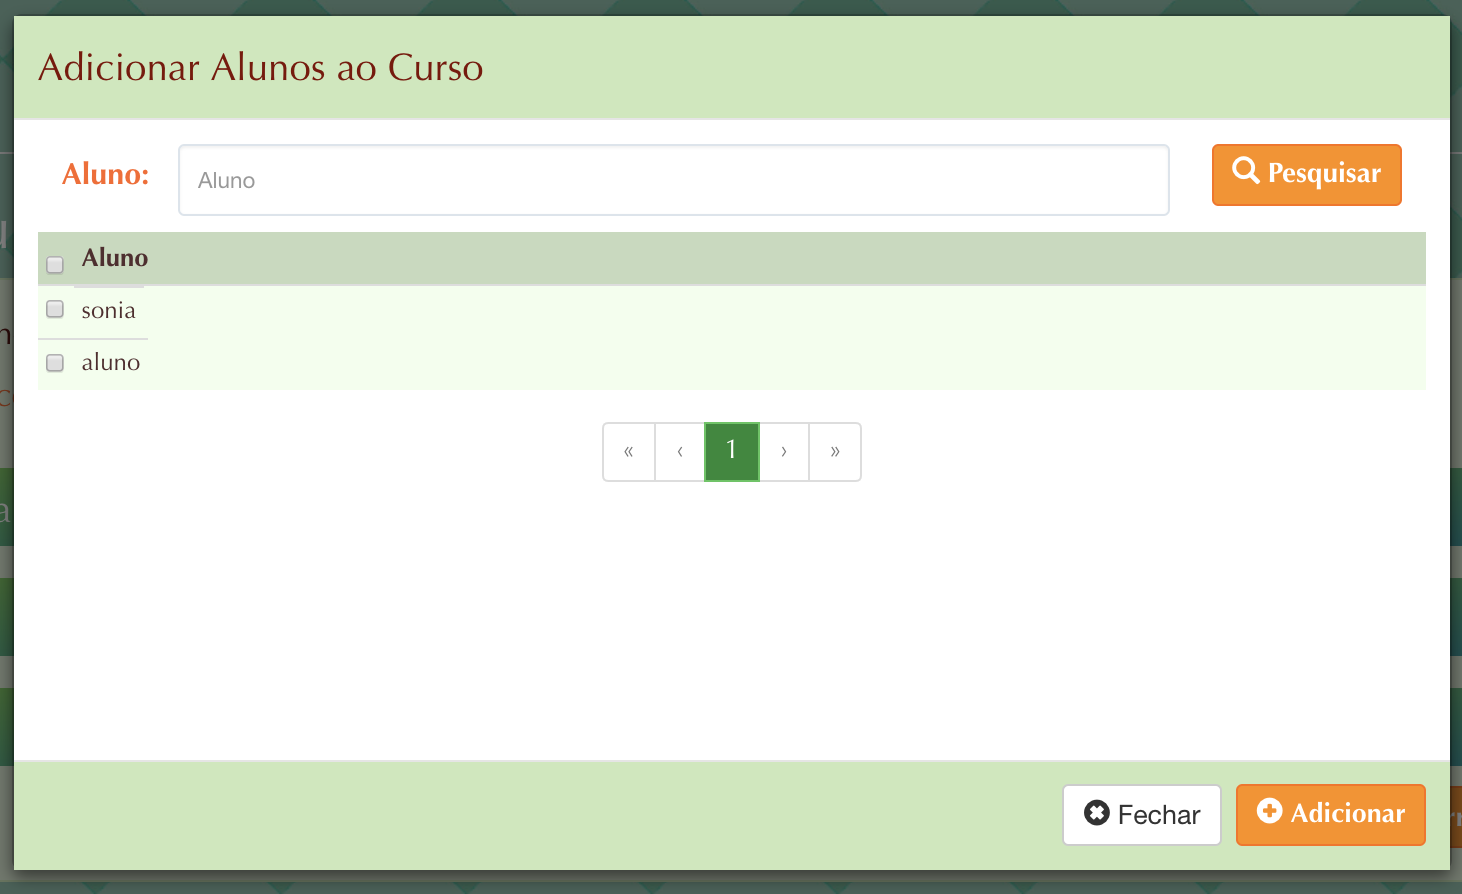
\includegraphics[scale=0.55]{images/proposta-img/Figura4-33.png}
  \caption{Tela de Adicionar Aluno ao Curso}
  \label{fig:Figura4-33}
\end{figure}

Por fim, o professor pode também adicionar aviso para os alunos. Essas avisos podem ser relacionado a prazos, dicas, links de auxílio ou qualquer conteúdo que o professor desejar adicionar. Cada aviso deve ter um título e descrição.

\begin{figure}[H]
  \centering
  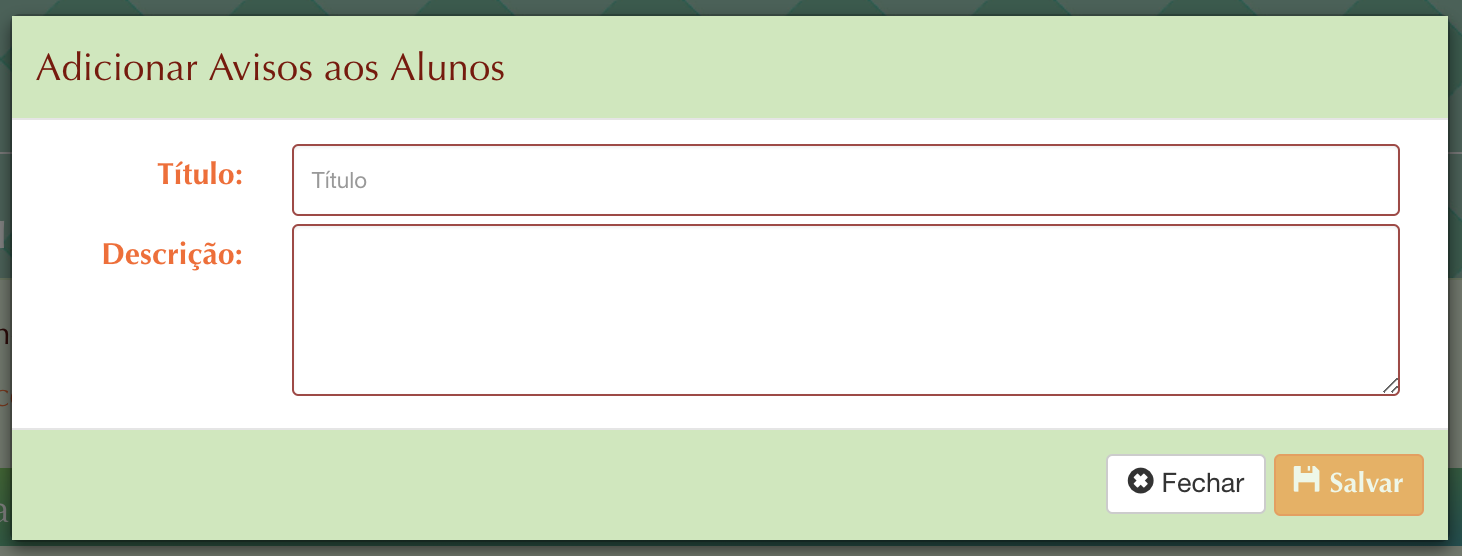
\includegraphics[scale=0.55]{images/proposta-img/Figura4-34.png}
  \caption{Tela de Adicionar Aviso ao Curso}
  \label{fig:Figura4-34}
\end{figure}

\subsection{Funcionalidades do Aluno}

O último perfil que o sistema disponibiliza é o de aluno, esse perfil pode buscar e participar de cursos da plataforma. Além disso, o aluno tem a possibilidade de visualizar o andamento, a colocação e a pontuação em todos os cursos que ele faz parte. A seguir mostraremos as ações que o usuário com esse perfil pode desempenhar no sistema.

\subsubsection{Cadastro de Aluno}

Como já foi dito, o aluno é o único usuário que pode se cadastrar no curso, para realizar esta ação é necessário acessar a página inicial e selecionar o botão “Cadastrar”. Este botão direcionar o aluno a tela mostrada na tela \figref{fig:Figura4-35}. Após preencher todos os campos e clicar em cadastrar, o aluno pode acessar o sistema da mesma forma que os demais usuário, vale destacar que ao entrar no sistema o aluno visualizar a tela inicial \figref{fig:Figura4-12}.

\begin{figure}[H]
  \centering
  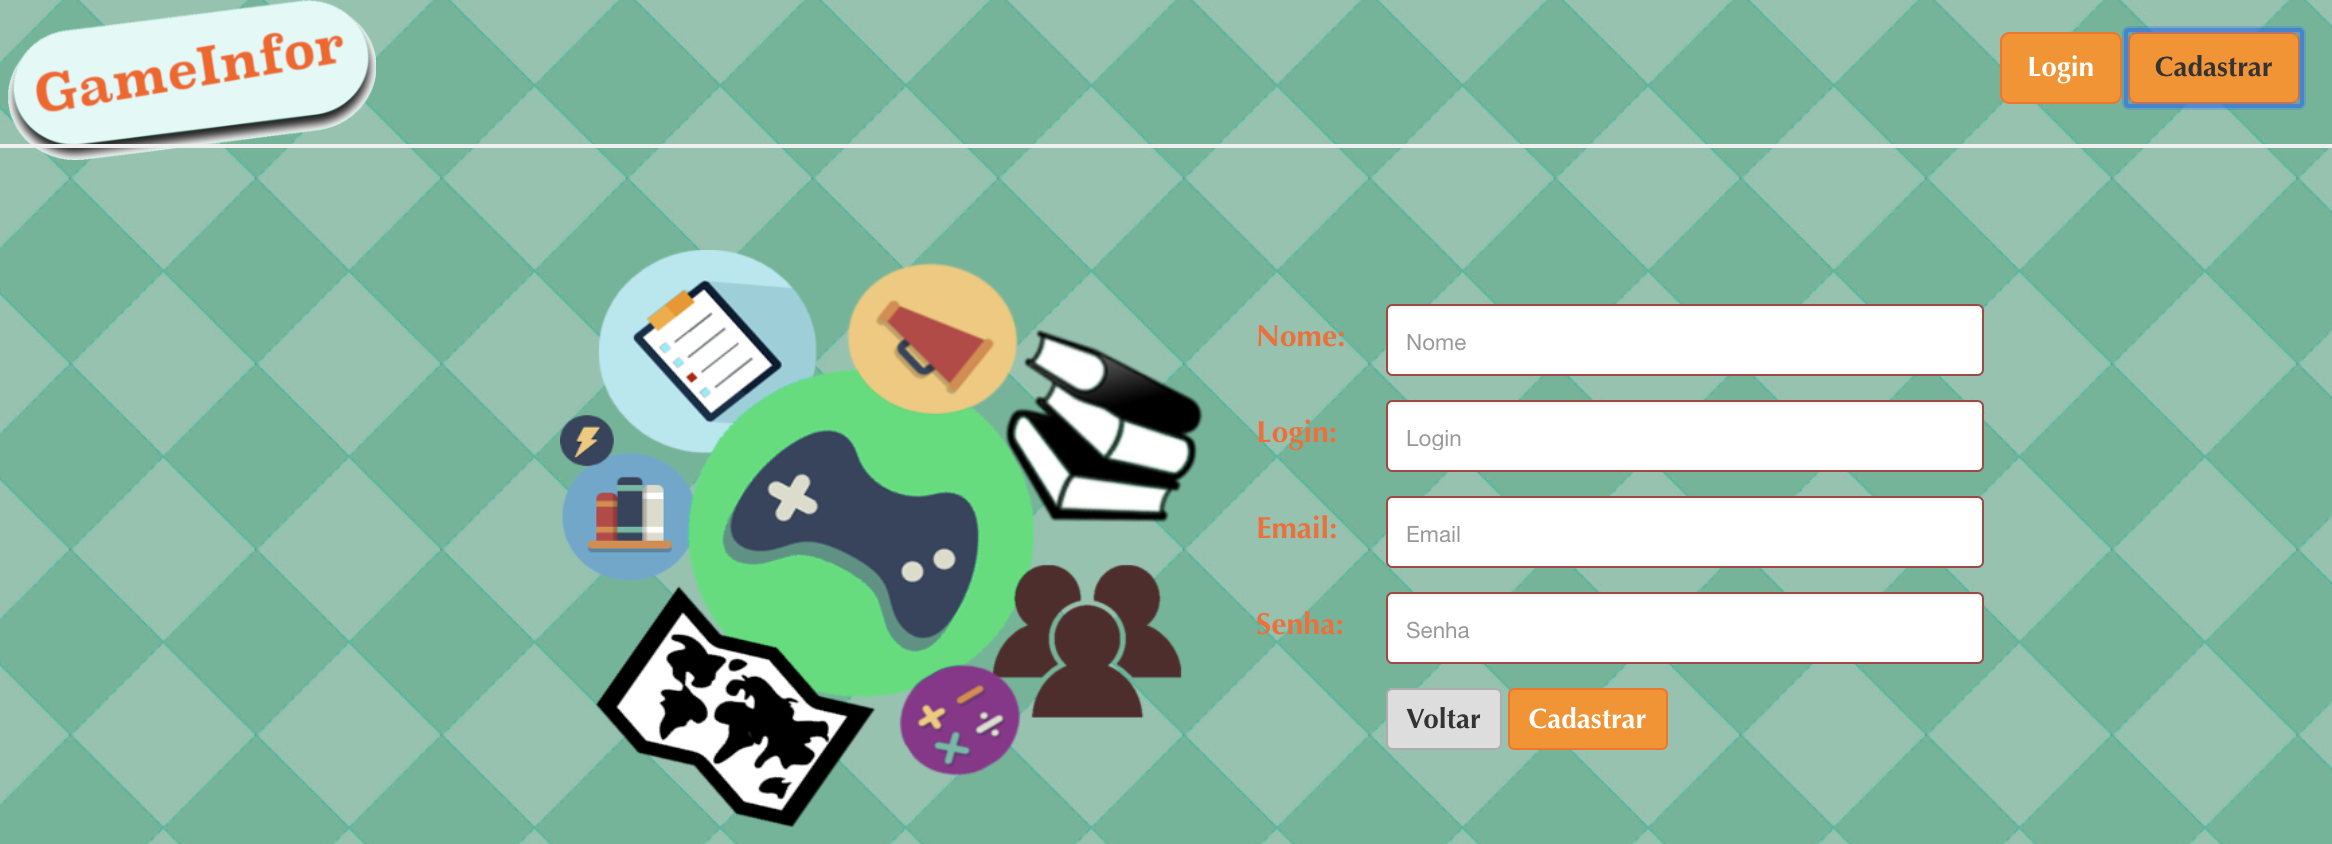
\includegraphics[scale=0.4]{images/proposta-img/Figura4-35.png}
  \caption{Tela de Cadastrar Aluno}
  \label{fig:Figura4-35}
\end{figure}

\subsubsection{Consultar Curso}

Após acessar a plataforma, o aluno tem a opção de consultar cursos do sistema, caso deseje realizar essa ação, o aluno deve clicar em "Consultar Cursos" ou ir no menu Aluno e selecionar a opção "Consultar Cursos". Após entrar na tela mostrada na tela \figref{fig:Figura4-36} o usuário pode pesquisar os cursos utilizando o filtro de nome ou categoria do curso, caso encontre resultados, é possível entrar no curso escolhido passando o código de acesso disponibilizado pelo professor, como é mostrado na imagem \figref{fig:Figura4-37}.

\begin{figure}[H]
  \centering
  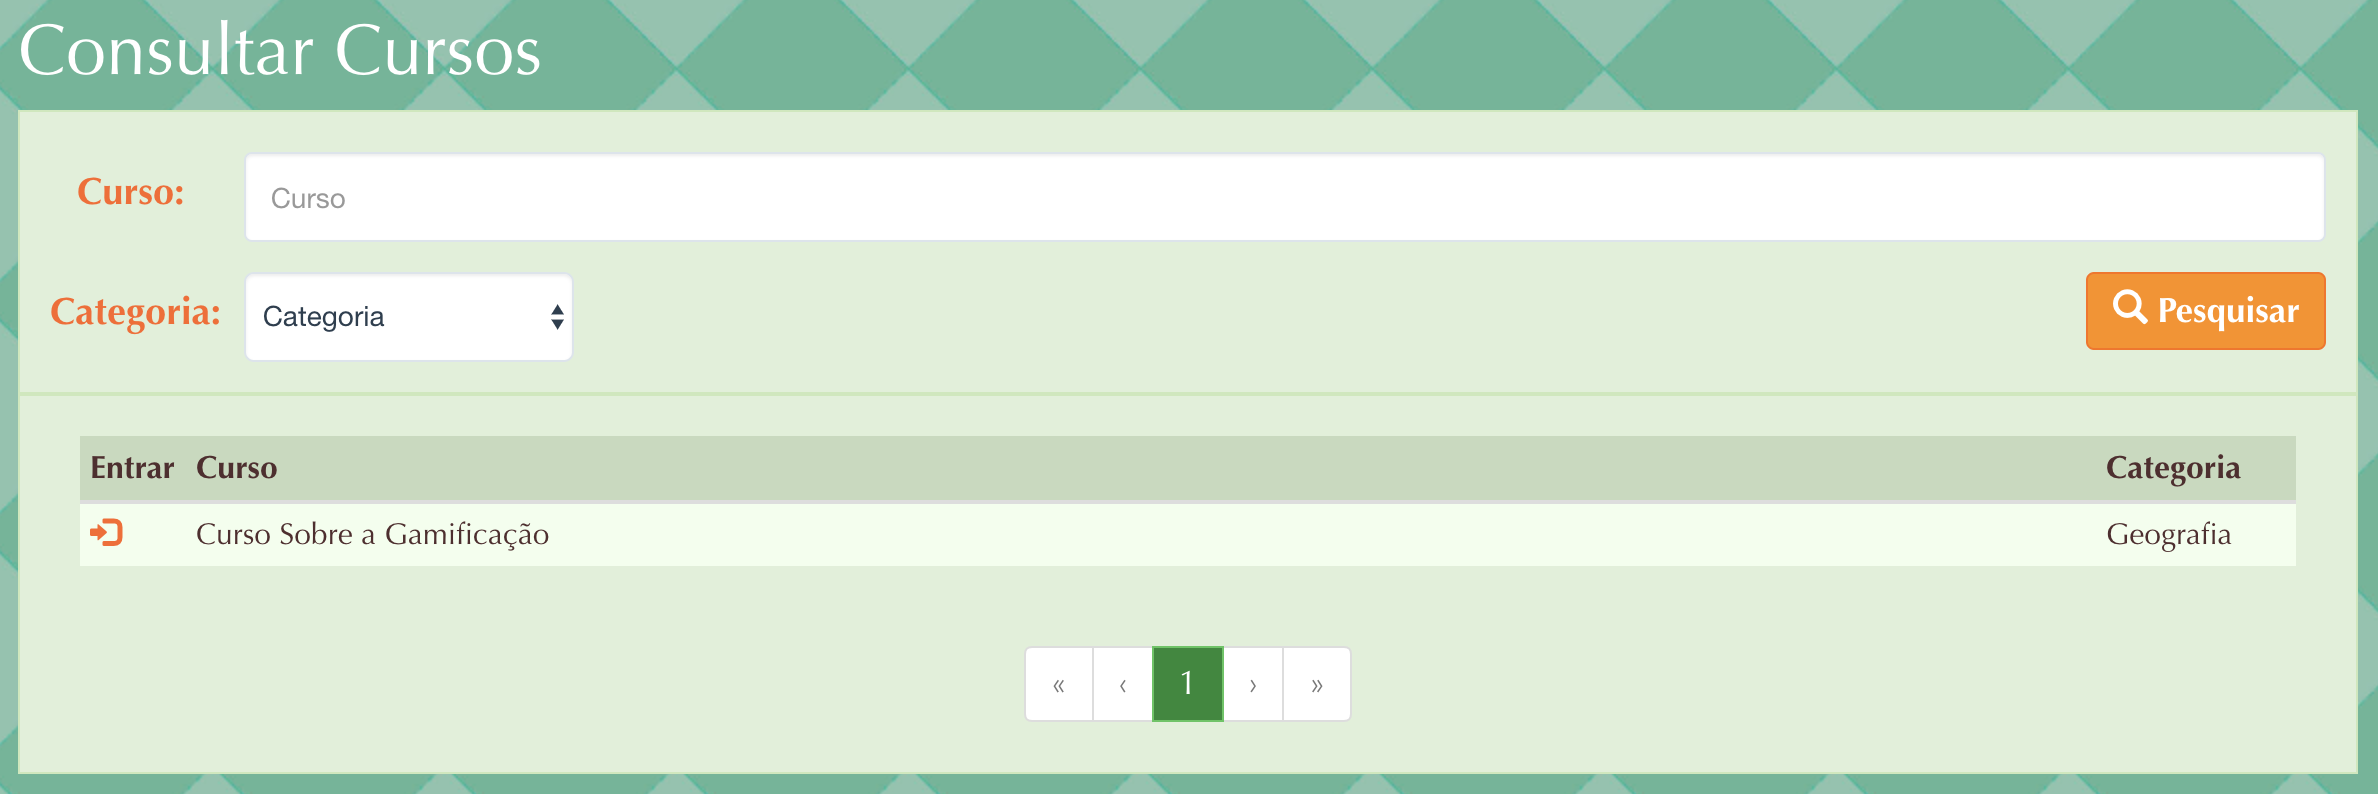
\includegraphics[scale=0.37]{images/proposta-img/Figura4-36.png}
  \caption{Tela de Consultar Curso}
  \label{fig:Figura4-36}
\end{figure}

\begin{figure}[H]
  \centering
  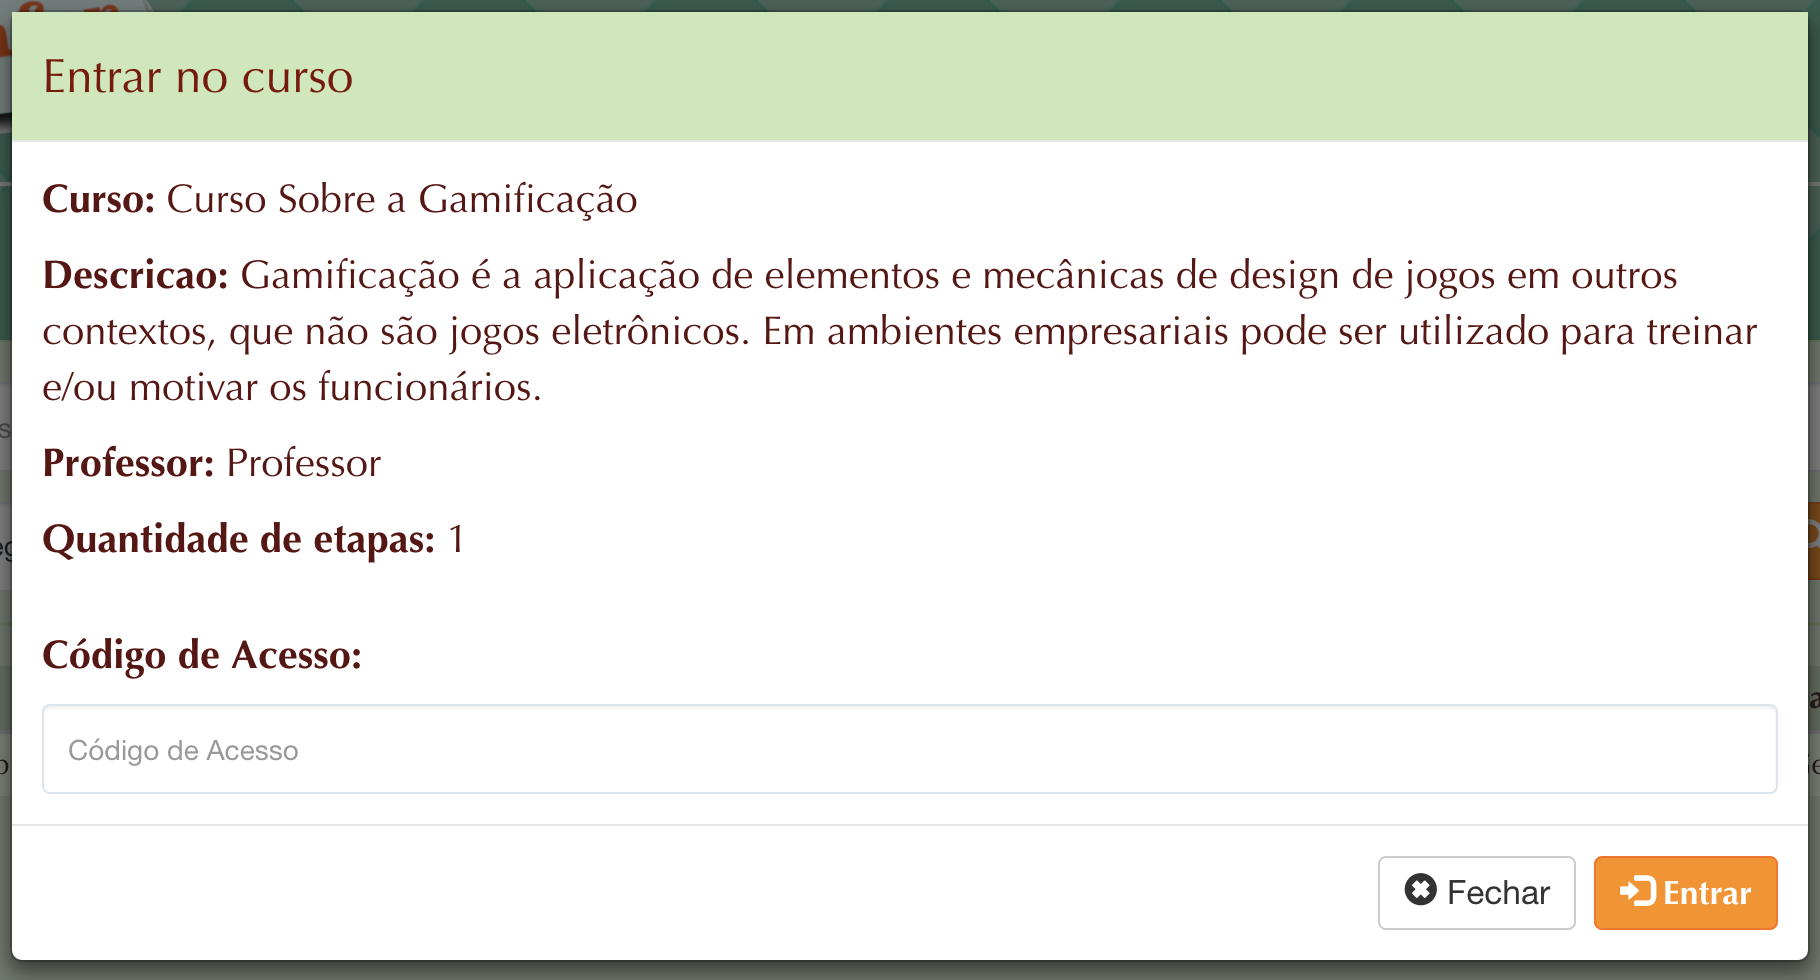
\includegraphics[scale=0.5]{images/proposta-img/Figura4-37.png}
  \caption{Tela de Entrar no Curso}
  \label{fig:Figura4-37}
\end{figure}

\subsubsection{Meus Cursos}

O usuário com este perfil tem a opção de acessar todos os cursos que ele faz ou fez parte na tela que pode ser acessada a partir do menu submenu "Meus Cursos" encontrado dentro do menu de aluno. Nessa tela, o estudante poderá  visualizar os cursos que estão em andamento na primeira parte da tela e os cursos que ele concluiu na segunda parte, como mostrado na tela \figref{fig:Figura4-38}.

\begin{figure}[H]
  \centering
  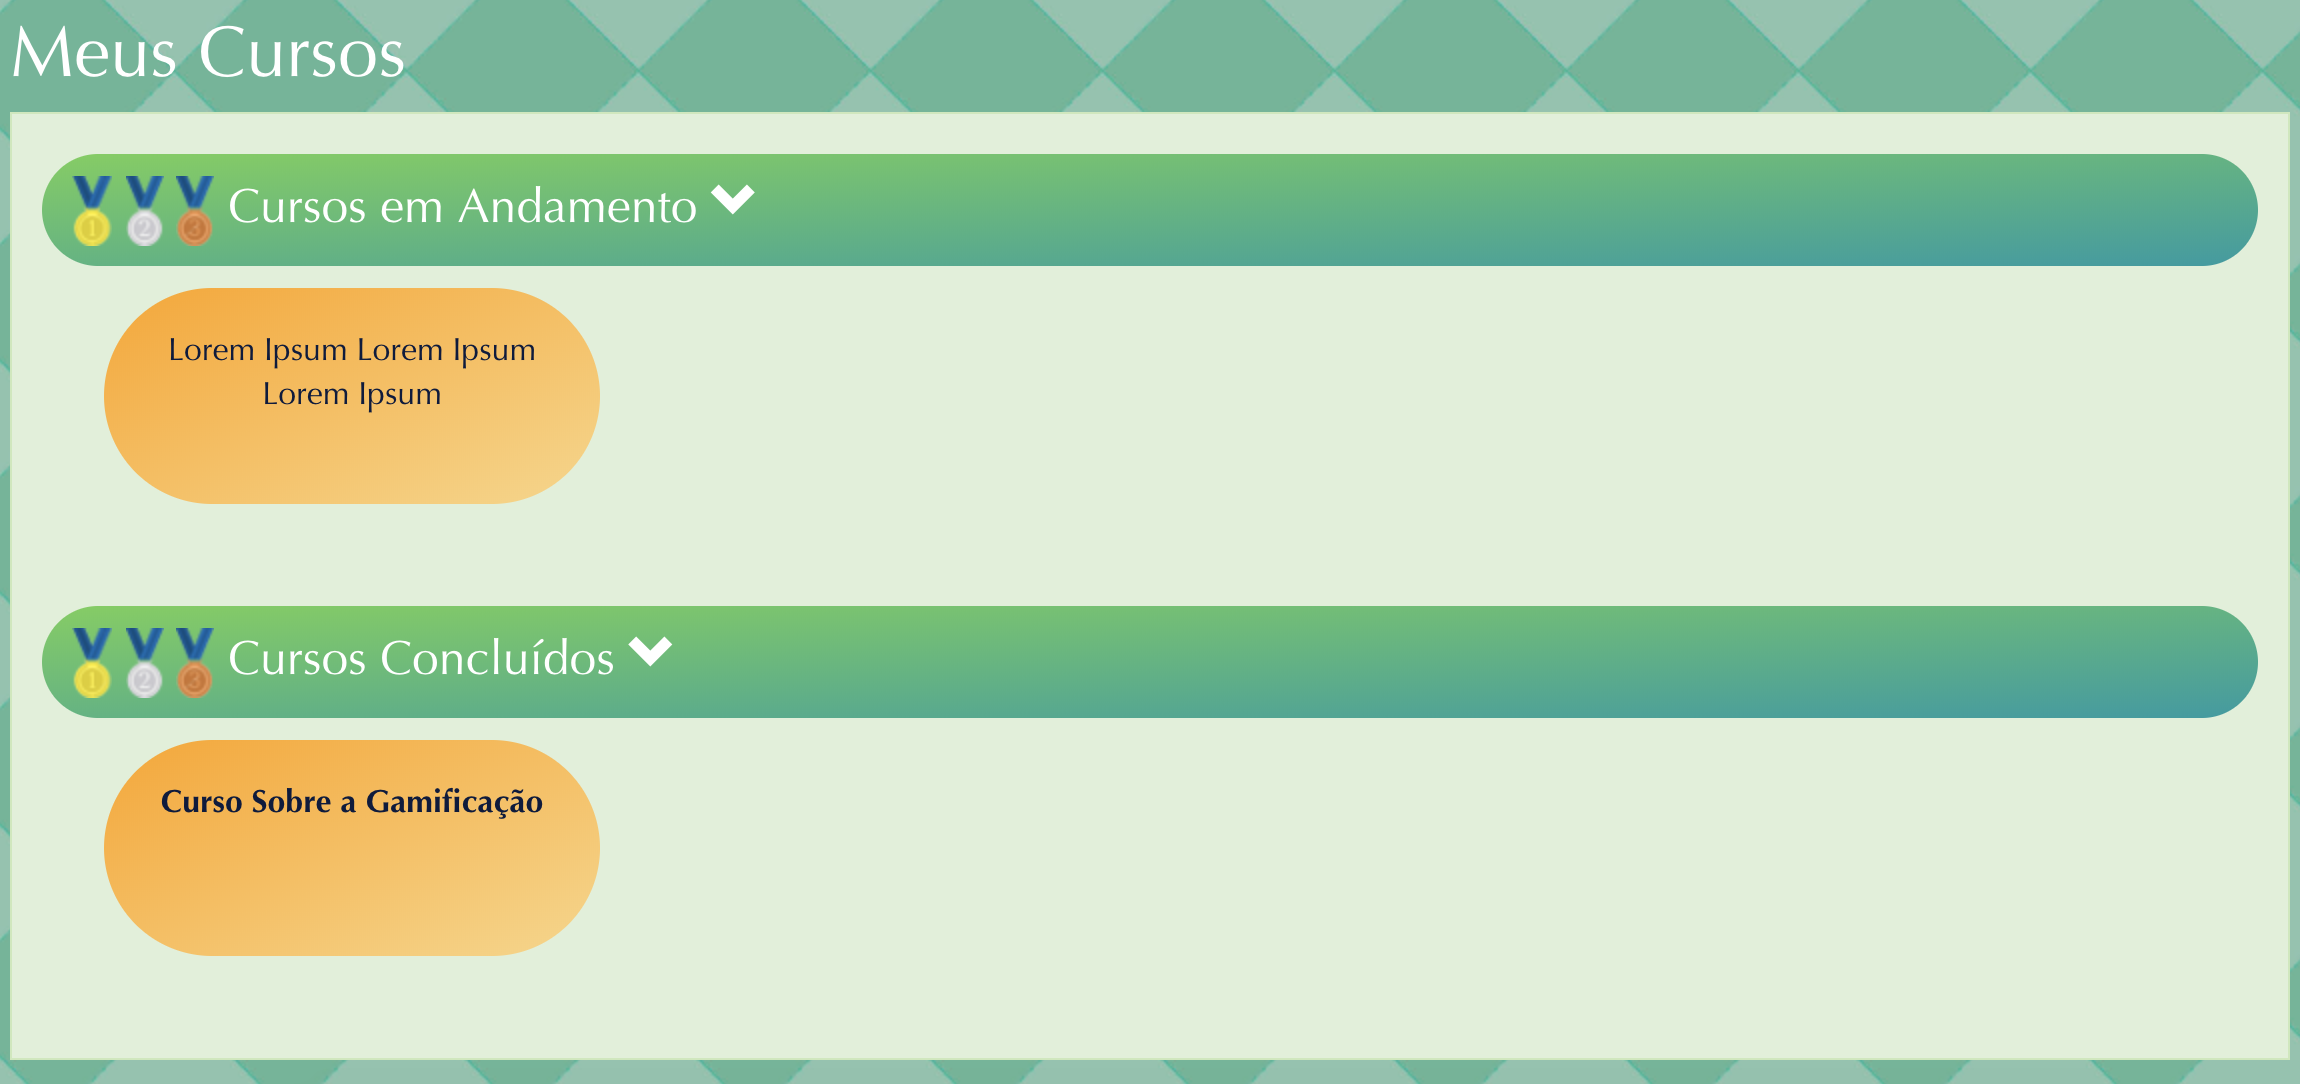
\includegraphics[scale=0.40]{images/proposta-img/Figura4-38.png}
  \caption{Tela de Meus Curso}
  \label{fig:Figura4-38}
\end{figure}
Após acessar um dos seus cursos em andamento, o aluno será direcionado para o tabuleiro do curso. Nesta tela, o aluno encontra o assunto abordado no curso, um botão para acessar os avisos deixados pelo professor e um tabuleiro gerado com todas as fases disponíveis como mostrado em  imagem \figref{fig:Figura4-39}. Com o intuito de evoluir no curso e chegar até a última etapa, o estudante deve vencer os desafios cadastrados. Clicando em na etapa o aluno encontrará um conteúdo em formato de texto e anexo, após o estudo do tópico abordado, a pessoa será confrontado com um jogo de perguntas selecionado pelo professor. A imagem da etapa pode ser visualizada em \figref{fig:Figura4-40}.

A medida em que o estudante receba a pontuação mínima para avançar nas etapas, essas serão desbloqueadas. Além disso, em cada fase, o aluno pode acessar o relatórios de todas as tentativas realizadas por ele. Cada relatório será composto da lista de perguntas, com as suas respostas corretas e incorretas como mostrado em \figref{fig:Figura4-41}. Ademais, para cada pergunta o aluno poderá verificar a explicação da resposta.

\begin{figure}[H]
  \centering
  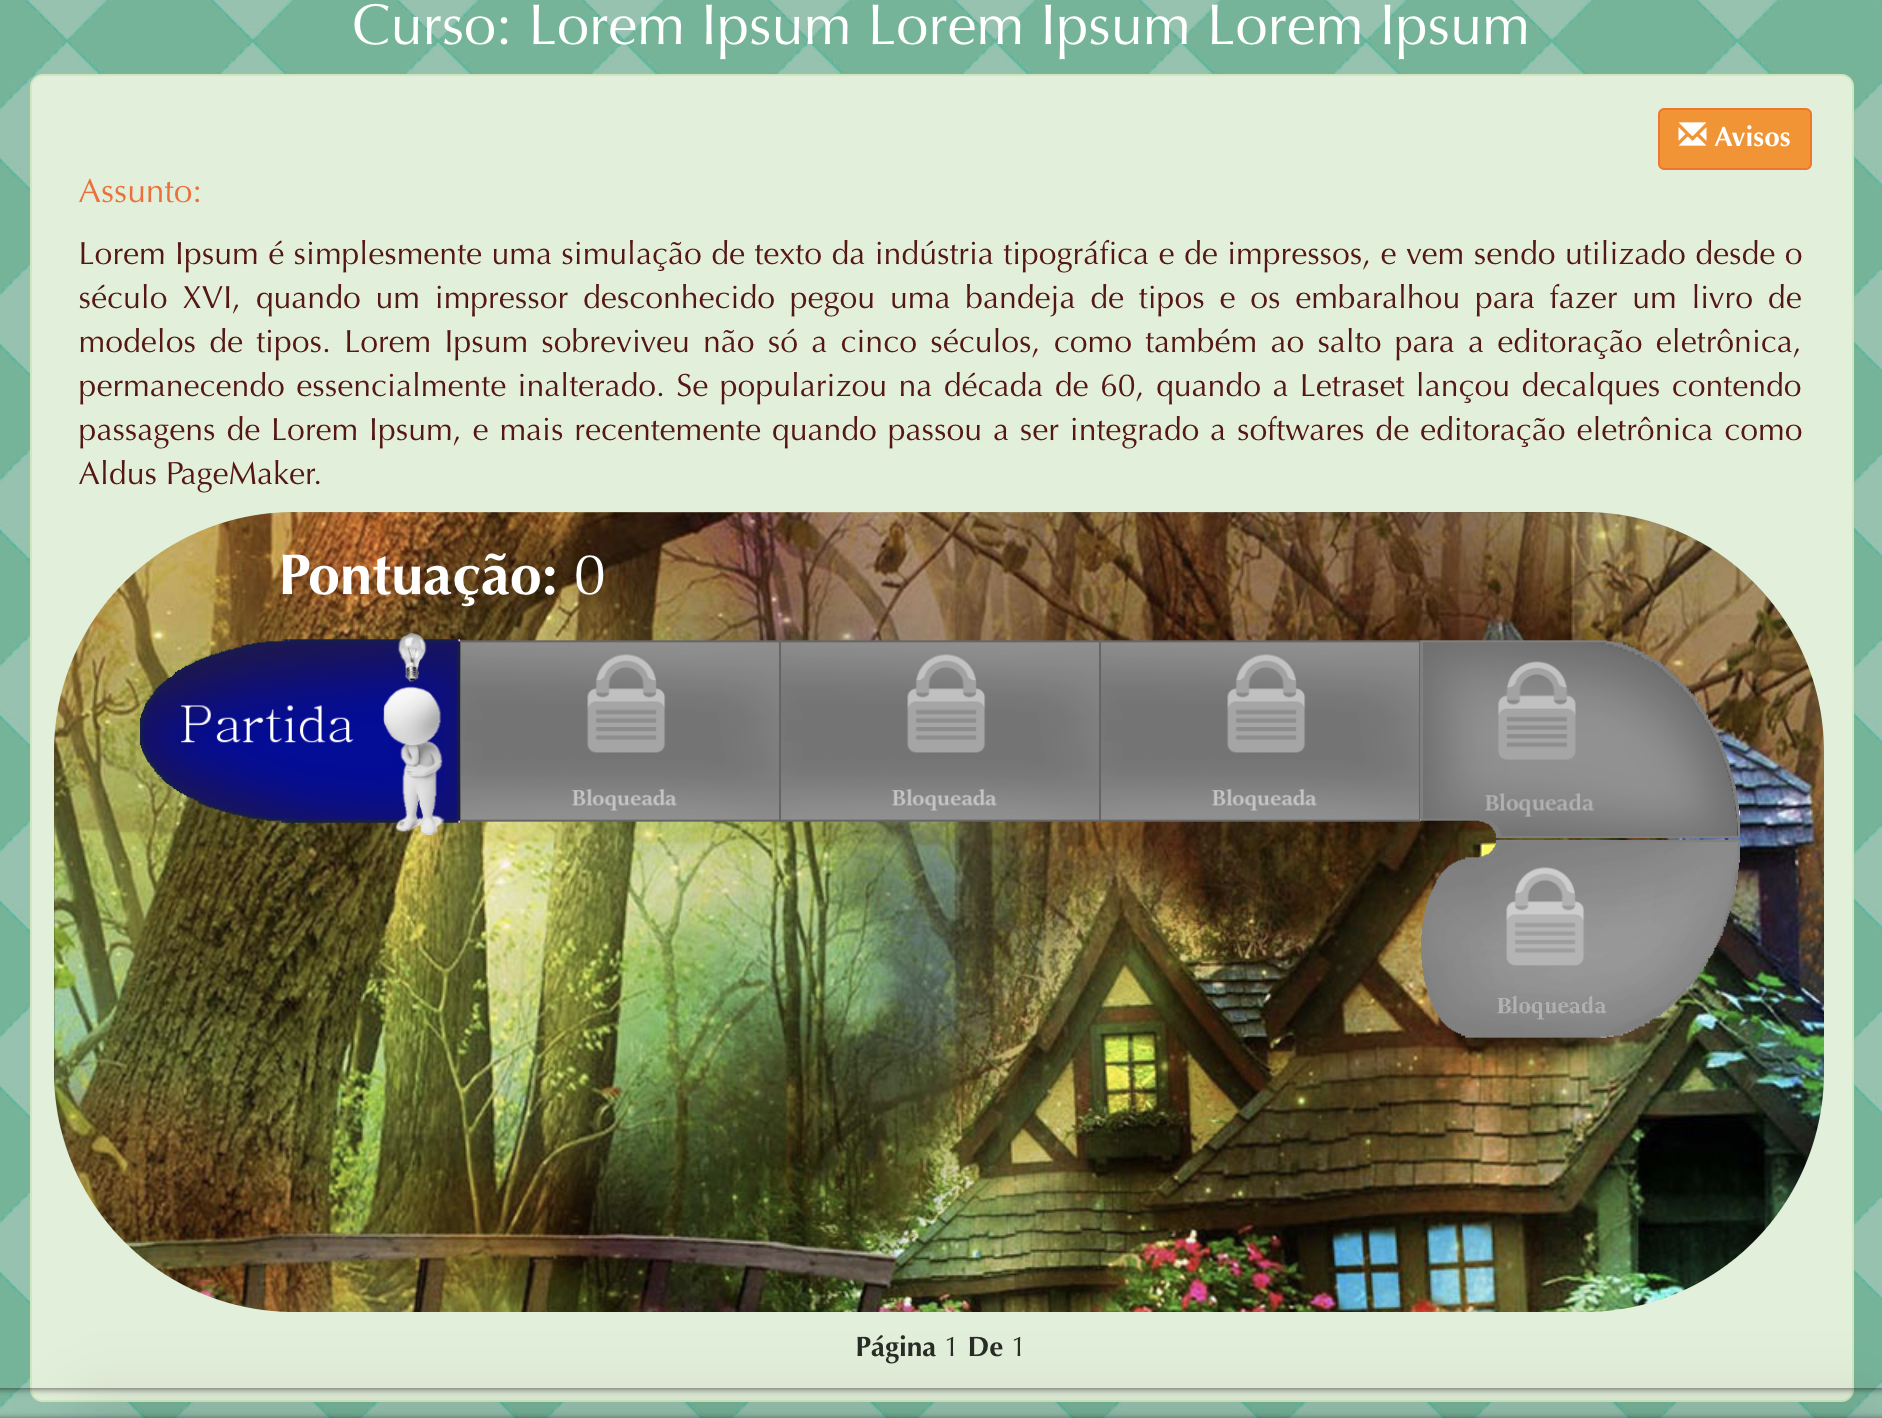
\includegraphics[scale=0.44]{images/proposta-img/Figura4-39.png}
  \caption{Tela de Tabuleiro do Curso}
  \label{fig:Figura4-39}
\end{figure}

\begin{figure}[H]
  \centering
  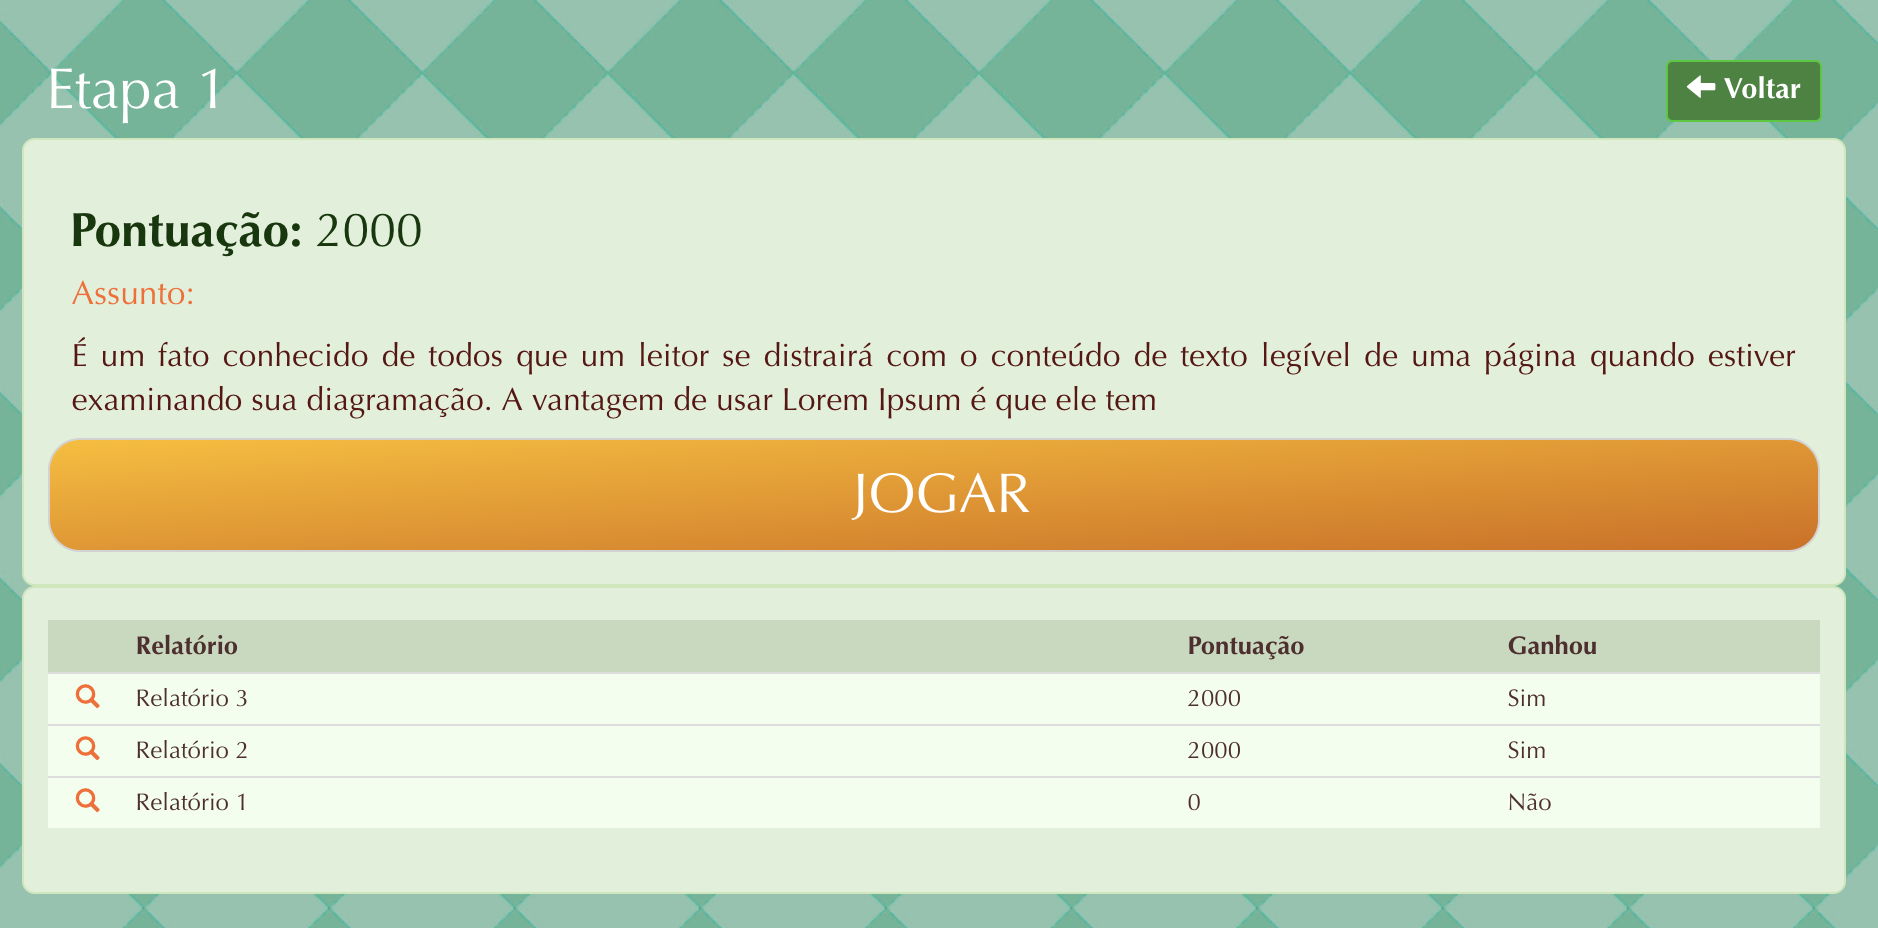
\includegraphics[scale=0.47]{images/proposta-img/Figura4-40.png}
  \caption{Tela de Etapa}
  \label{fig:Figura4-40}
\end{figure}

\begin{figure}[H]
  \centering
  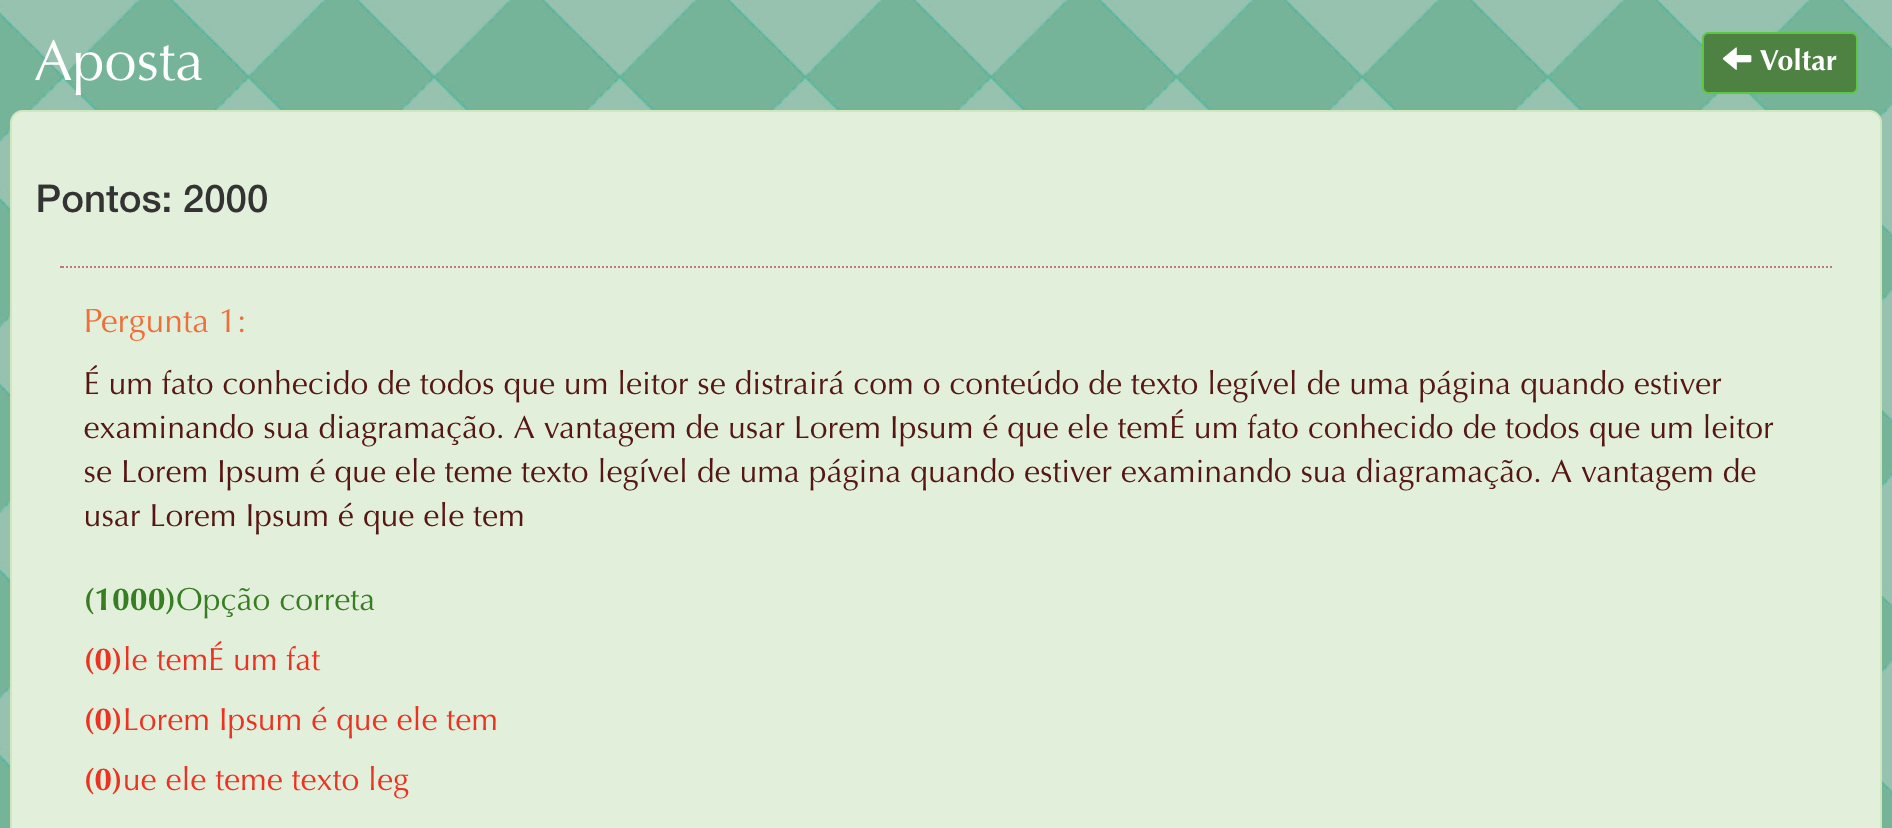
\includegraphics[scale=0.44]{images/proposta-img/Figura4-41.png}
  \caption{Tela de Relatório da Etapa}
  \label{fig:Figura4-41}
\end{figure}

\subsubsection{Ver Meu Andamento}

A última funcionalidade disponível ao aluno é o acompanhamento de andamento nos curso. Essa tela deve ser acessada através do menu do aluno. Após clicar em "Ver meu Andamento" poderá ver todos os cursos que ele faz parte, a etapa em que ele parou, a pontuação atual e a sua colocação entre todos os aluno.

\begin{figure}[H]
  \centering
  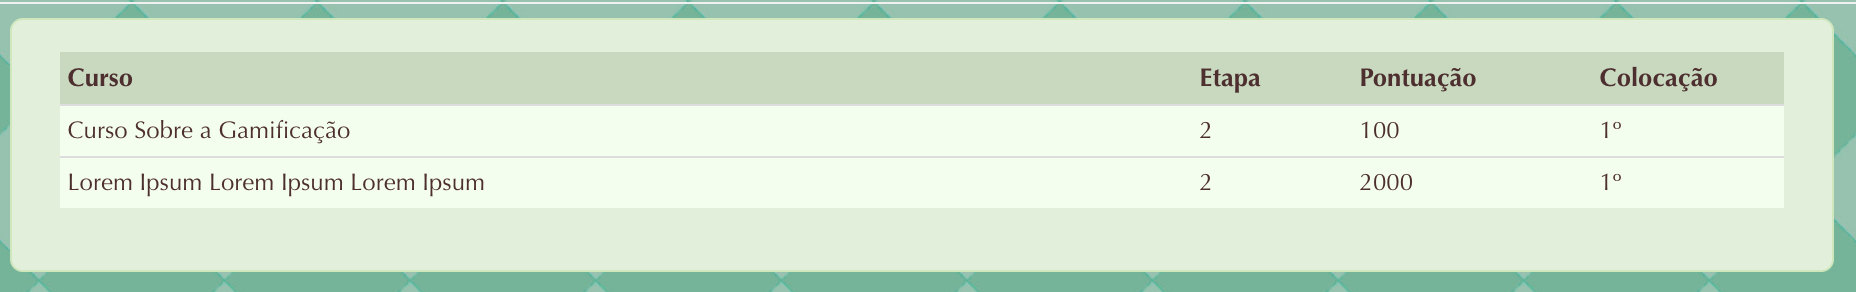
\includegraphics[scale=0.46]{images/proposta-img/Figura4-42.png}
  \caption{Tela de Relatório da Andamento}
  \label{fig:Figura4-42}
\end{figure}